\documentclass{article}
\usepackage[utf8]{inputenc}
\usepackage{amsmath, amssymb, amsfonts}
\usepackage{tikz}
\usepackage{pgfplots}
    \pgfplotsset{compat=newest}
\usepackage{cancel}
\usepackage[margin=3cm]{geometry}
%\usepackage{enumitem} % Allow tight lists
\usepackage{gensymb} % for degree symbol
\usepackage{tikzscale}
  

%\title{Robust control system development for VTOL-to-fixed wing flight %transition with the EcoSoar UAV}
%\author{Robert Hedman}
%\date{April 2019}


\begin{document}

\begin{titlepage}
    \begin{center}
        %\vspace*{1cm}
 
        \huge
        \textbf{Robust control system development for VTOL-to-fixed wing flight transition with the EcoSoar UAV}
 
        \vspace{0.5cm}
        \LARGE
        A thesis in Automatic Control
 
        \vspace{1.5cm}
 
        \textbf{Robert Hedman\\}
        \today
        \vspace{0.6cm}

        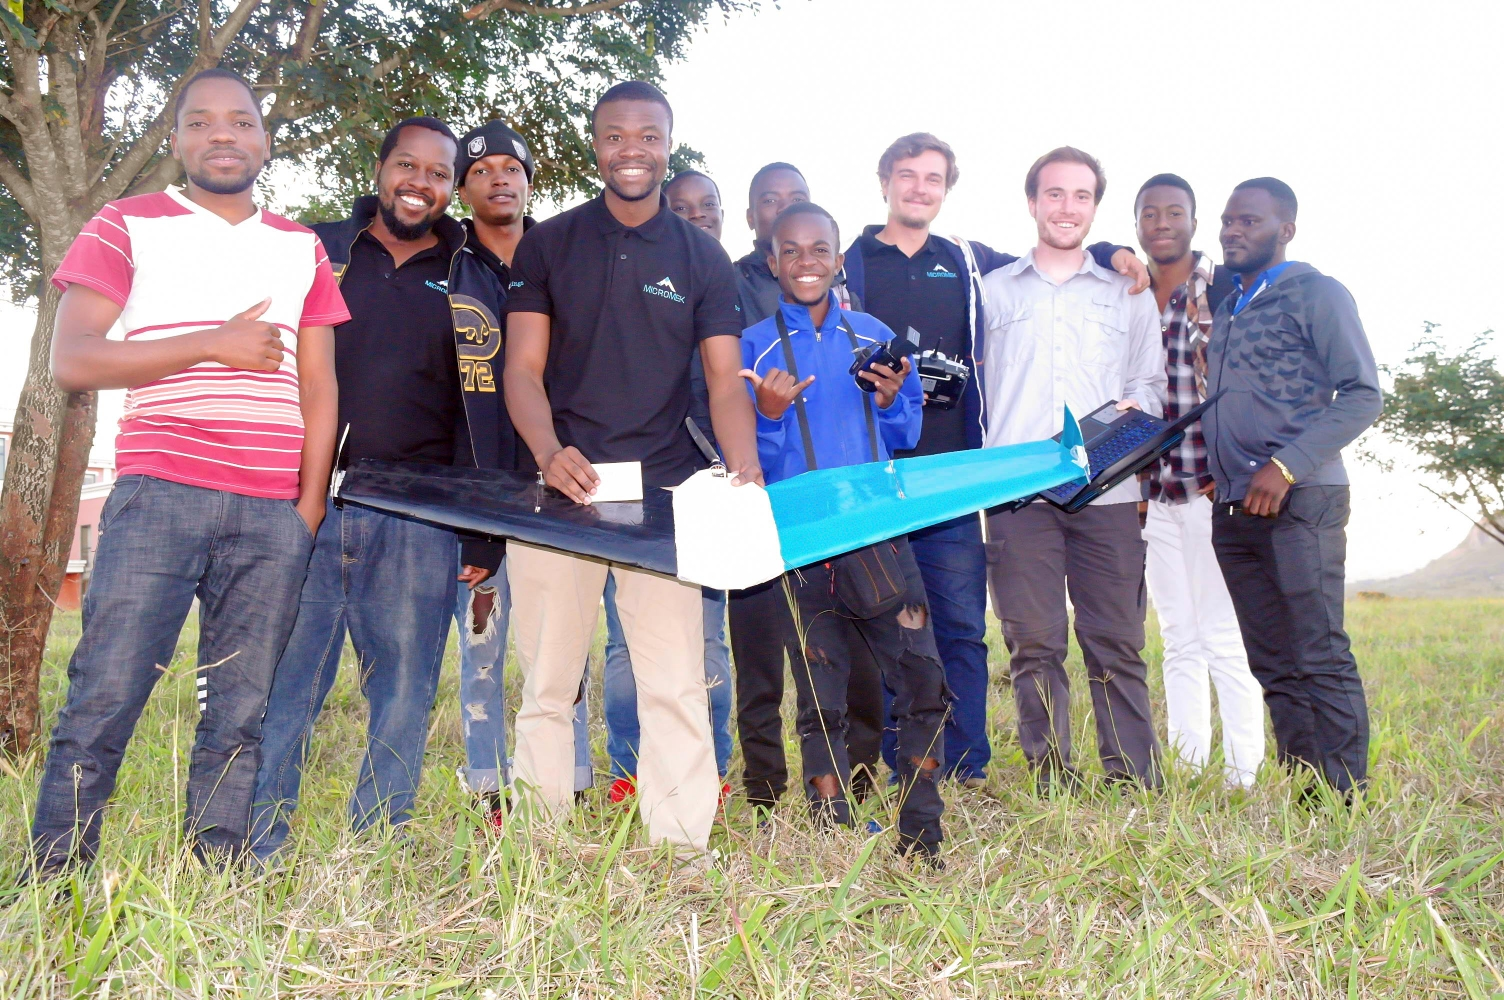
\includegraphics[width=0.9\textwidth]{coverphoto.jpeg}
 
        \vfill
 
        A thesis presented for the degree of\\
        Masters of Science / Civil Engineer
 
        \vspace{0.6cm}
 
        \Large
        Department of Computer Science, Electrical and Space Engineering\\
        Luleå University of Technology\\
        %\textit{Supervisors:} K. \textsc{Atta}, K. \textsc{Kochersberger}\\
        %\textit{Supervisors:} K. \textsc{Kochersberger}\\
        \textit{Examinator:} G. \textsc{Nikolakopoulos}

 
    \end{center}
\end{titlepage}

\abstract
A non linear quaternion based attitude controller of type P2 controller, together with a sensitivity normalizing function for the control surfaces has been simulated and implemented on a flying fixed wing with non vectored engines.
In simulations the controller worked well in all flight modes, hovering, transition and flying, and also rejected a simple wind disturbance in all modes.
The first implementation on hardware did not work due to programming errors causing crashes with unrepairable damages.
The second aircraft was built out of a piece of plywood to further simplify the testing and tolerate more crashes.
A non-existing airfoil, flat plate, has no effects due to camber and is therefor easier to both simulate and tune.
The controller worked acceptable in reality, but does need further tuning.
Due to time constraints the weighing of airflow inside and outside the propeller wash could not be fully determined resulting in different gain in the different flight modes, but initial estimation of the parameters were enough to achieve robust, stable hovering transitioning and flying even in quite strong wind (more than 5 m/s).
The controller was never implemented on a EcoSoar due to time constraints, but the proof of concept flying piece of plywood proved the controller feasible for future embedding in a modified EcoSoar. 


\newpage
\section*{\textit{Acknowledgements}}

I would like to extend a special thanks to Dr. Kochersberger at Virginia Tech who supplied me with the materials to finish this thesis.
Fellow students, Avery and Brianna, also helped me a lot in understanding the building of an EcoSoar and general aerodynamics.
My friend and teacher at LTU, K. Atta, also deserves a very big thanks for the many hours over a really bad phone connection he helped me try different control, and modeling, approaches.

I also want to extend a very warm thank you to Montford Special Needs College in Malawi for allowing me to stay there together with my wife during this thesis.
The staff provided all the support needed to become integrated with the local culture and helping out with practical issues such as getting a car, finding the hospital and providing a safe circle of friends.

Without XP-EL this thesis would not have been possible, they donated a 3D-printer that now resides with locals improving Malawi bit by bit.

\newpage

\tableofcontents

\newpage
\section{List of Variables}
%\begin{itemize}[topsep=0pt,itemsep=-1ex,partopsep=1ex,parsep=1ex]
\begin{center}\begin{tabular}{| c | c |} 
    $L_L$       & Lift from left wing \\
    $L_R$       & Lift from right wing \\
    $D_L$       & Drag from left wing \\
    $D_R$       & Drag from right wing \\
    $F_L$       & Lift due to aileron deflection, left side, outside propeller wake \\
    $F_{L_T}$   & Lift due to aileron deflection, left side, inside propeller wake \\
    $F_R$       & Lift due to aileron deflection, right side, outside propeller wake \\
    $F_{R_T}$   & Lift due to aileron deflection, right side, inside propeller wake \\
    $D_{\alpha_L}$ & Drag due to aileron deflection, left side, outside propeller wake \\
    $D_{\alpha_{L,T}}$ & Drag due to aileron deflection, left side, inside propeller wake \\
    $D_{\alpha_{R}}$ & Drag due to aileron deflection, right side, outside propeller wake \\
    $D_{\alpha_{R,T}}$ & Drag due to aileron deflection, right side, inside propeller wake \\
    $L_{W_L}$ & Lift from left winglet \\
    $L_{W_R}$ & Lift from right winglet \\
    $D_{W_L}$ & Drag from left winglet \\
    $D_{W_R}$ & Drag from right winglet \\
    $S_a$  & Surface area of one aileron, parts outside propeller wake \\
    $S_{a_w}$ & Surface area of one aileron, area inside propeller wake \\
    c.g.    & center of gravity (point) \\
    $T_L$   & Thrust from left propeller \\ 
    $T_R$   & Thrust from right propeller \\
    $S_w$   & Area of one wing, area outside of propeller wake \\
    $S_{w_w}$ & Area of one wing, area inside propeller wake \\
    $S_W$   & Area of one winglet \\
    $x_f$   & distance in $x$ from c.g. to aileron force \\
    $x_T$   & distance in $x$ from c.g. to thrust force \\
    $x_{ac}$& distance in $x$ from c.g. to wing aerodynamic center \\
    $x_W$   & distance in $x$ from c.g. to winglet force \\
    $y_T$   & distance in $y$ from c.g. to thrust force \\
    $y_f$   & distance in $y$ from c.g. to aileron force \\
    $y_{ac}$& distance in $y$ from c.g. to wing aerodynamic center \\
    $y_w$   & width of propeller wake \\ 
    $b$     & wingspan \\
    $z_W$   & distance in $z$ from c.g. to winglet force
\end{tabular} \end{center}
\newpage

\section{Background}
Virginia Tech, a University in Virginia, USA, has developed a fixed wing drone called the EcoSoar; a flying wing.
It is an aircraft designed for fabrication, operation and maintenance in low-
resource environments.
The total cost of one EcoSoar is only around 350 USD when costs for all tools and materials have been accounted for and spread over ten aircraft.

EcoSoar has been successfully flown in Malawi at
the test corridor established by UNICEF in Kasungu,
where a simulated payload of dried blood spot sam-
ples (used for HIV testing) was delivered 19 km from
a remote health clinic to the Kasungu airport. The
aircraft is constructed of poster-board and 3D printed
parts, making it easy to source in Malawi and low-
cost to repair if damaged.

Many flight operations occurring in Africa are converging on hybrid aircraft designs where the aircraft functions as a quadcopter in takeoff and landing but is capable of higher speed flight in a fixed wing configuration.

EcoSoar can currently be launched with a big bungee-cord or with a custom built launcher. It thus needs a field to both take off and land in since it can only land on its belly similar to that of any normal aircraft.
Modifying the EcoSoar to have two engines, one on the front of each wing, instead of the current design of having one at the back, might allow it to hover, take off and land vertically eliminating the need for a launching system as well as the requirement of a big field for take-off and landing.

Adding VTOL capacity to this drone would greatly increase its range of possible missions and thus help humanitarian efforts centered around EcoSoar in Malawi.

To achieve VTOL not only is hardware modifications necessary but also a new control scheme is necessary.

\section{Problem Forumulation}
This thesis will attempt to solve the problem of mathematically modeling a flying fixed wing, develop a VTOL capable model based controller that can handle both hovering, transitioning into flying and flying, and finally implement the controller on the Pixhawk controller onboard the aircraft.
Altering the aerodynamics of the EcoSoar is out of the scope for this thesis as is embedding the controller into fully fledged flight control system for example QGroundControl.
The project takes place in Malawi with very limited supply of electronics, spare parts, electricity, tools and lab equipment.

%Typically included as a subsection of the Introduction.
%Often accompanied by delimitations - statments about what is out of scope of the project.

%Formulation is incorrectly spelled.

\section{Theory}
To develop this controller some basic concepts are required.
\subsection{State Space}
Many systems can be written as a set of differential equation.

Physical systems may sometimes be mathematically modeled by state space representation, given that it can be written on the same form as equation \ref{eq:generalstatespace} below.
\begin{equation}
    \dot{\bar{x}} = f(\bar{x}) + g(\bar{u},\bar{x})
    \label{eq:generalstatespace}
\end{equation}
The states, $\bar{x}$ are related by a set of first order differential equations and some input.

Systems can have one input and one state/output, called Single Input Single Output (SISO), or have either multiple input or outputs or both; Multiple Input Multiple Output (MIMO) systems.
A system with several states, i.e. $\bar{x}$ being a vector, and several inputs, i.e. $\bar{u}$ being a vector is thus represented by a set of functions $\bar{f}$ and $\bar{g}$.

From basic fundamental physical laws, e.g. newtons laws, a set of differential equation for many physical systems can be derived.
Once the state space equations are known simulating the system is only a matter of choosing a differential equation solver.
Simulink has built in solver for these equations over time making it easy to simulate the system once the equations are known.

\subsection{State estimation/observers}
A full state vector may not always be exactly measurable so estimating it is of importance.
The Pixhawk PX4 firmware already includes an extended Kalman filter for estimating the position and attitude from an angular rate sensor, accelerometer, barometer and magnetometer.
For this project the built in Kalman filter will be used to estimate the state with which the control system will act upon.

\subsection{Reference Frames}
When working with rigid bodies in 3d space a reference system is needed.
In most of airplane dynamics for small scale aircraft the standard is a Cartesian coordinate system with the x-axis aligned with North, y-axis aligned with East and the z-axis pointing down.
The body frame is similar, x-axis pointing forwards, y-axis along right wing and z-axis through the belly of the aircraft, i.e. down when flying normally.
This correspond to the well used Roll-Pitch-Yaw system.\cite{nelson}

\subsection{Quaternions}
Euler angles are intuitive but suffer from singularities.
Since normal aircraft normally do not spend time pointing straight up these singularities do not matter too much, but a VTOL capable tail-sitter will, so using quaternions is beneficial.

A quaternion, $\bold{q}$ is a four dimensional hyper complex number.\cite{P2}
\begin{equation}
 \mathbf{q} = q_0 + q_1 \mathbf{i} + q_2 \mathbf{j} + q_3 \mathbf{k}
\end{equation}
where $i^2 = j^2 = k^2 = ijk = -1$.\cite{Sola2016}
The imaginary part can be referenced to as the vector part and $q_0$ the scalar part.
The conjugate of a quaternion is defined as
\begin{equation}
     \mathbf{q^*} = q_0 - q_1 \mathbf{i} - q_2 \mathbf{j} - q_3 \mathbf{k}
\end{equation}
The quaternion can also be represented as a vector:
\begin{equation}
     \bold{q} = \left[
     \begin{matrix}
     q_0 &q_1 &q_2 &q_3
     \end{matrix}\right]
\end{equation}
The norm of a quaternion is defined by
\begin{equation}
    ||\mathbf{q}|| = \sqrt{\mathbf{q} \otimes \mathbf{q}^*} = \sqrt{q_0^2 + q_1^2 + q_2^2 + q_3^2}
\end{equation}
If the norm of a quaternion is equal to $1$ it is a unit quaternion.
Unit quaternions are very computationally efficient at describing rotations in 3D.
They also do not suffer from any singularities like the common Roll-Pitch-Yaw / Euler angles system.
Unit quaternions can always be written as
\begin{equation}
    \mathbf{q} = \left[\begin{matrix} cos \theta &\\ \mathbf{u} sin \theta\end{matrix}\right]
\end{equation}
where $\mathbf{u}$ is the vector $\left[\begin{matrix} q_1 & q_2 & q_3 \end{matrix}\right]$
describing the axis of which to rotate around and $\theta$ is proportional to the amount of rotation about that axis.
Multiplying unit quaternions yield a unit quaternion describing the joint rotation of the two initial quaternions.
The conjugate of a quaternion gives the opposite rotation direction around the same vector.
This can correspond to going from a world frame to body frame, or vice versa.
Multiplying a reference quaternion describing a set orientation for an object in 3D with the conjugate of its actual quaternion therefore gives the error in orientation, attitude.

A more in depth description of quaternions and their mathematics please see \cite{Sola2016}.

%\subsection{Equations of Motion, in body frame}


\subsection {Basic aerodynamics}
An object moving through a medium displaces mass in the medium it travels through,
A wing moving through the air will displace air particles.
If the total movement of the particles generate a net momentum a force will be generated on the object displacing them, in this case the wing.

The air will thus excert pressure on the wing and it is useful to consider the pressure distribution.
By integrating the pressure distribution over the entire surface of the wing one can find the center of pressure.\cite{aerodynamics}
If the center of pressure and center of gravity are not aligned a torque will also be generated.
The equivalent force and moment can be placed at the center of pressure to simplify calculations.
The aerodynamic force can be split into two parts, one in line with the incoming airflow and one perpendicular to it.
These are usually denoted Lift and Drag forces, see figure \ref{fig:liftdrag} for an illustration of the Lift and Drag forces on an airfoil.

\begin{figure}[h]
    \center
    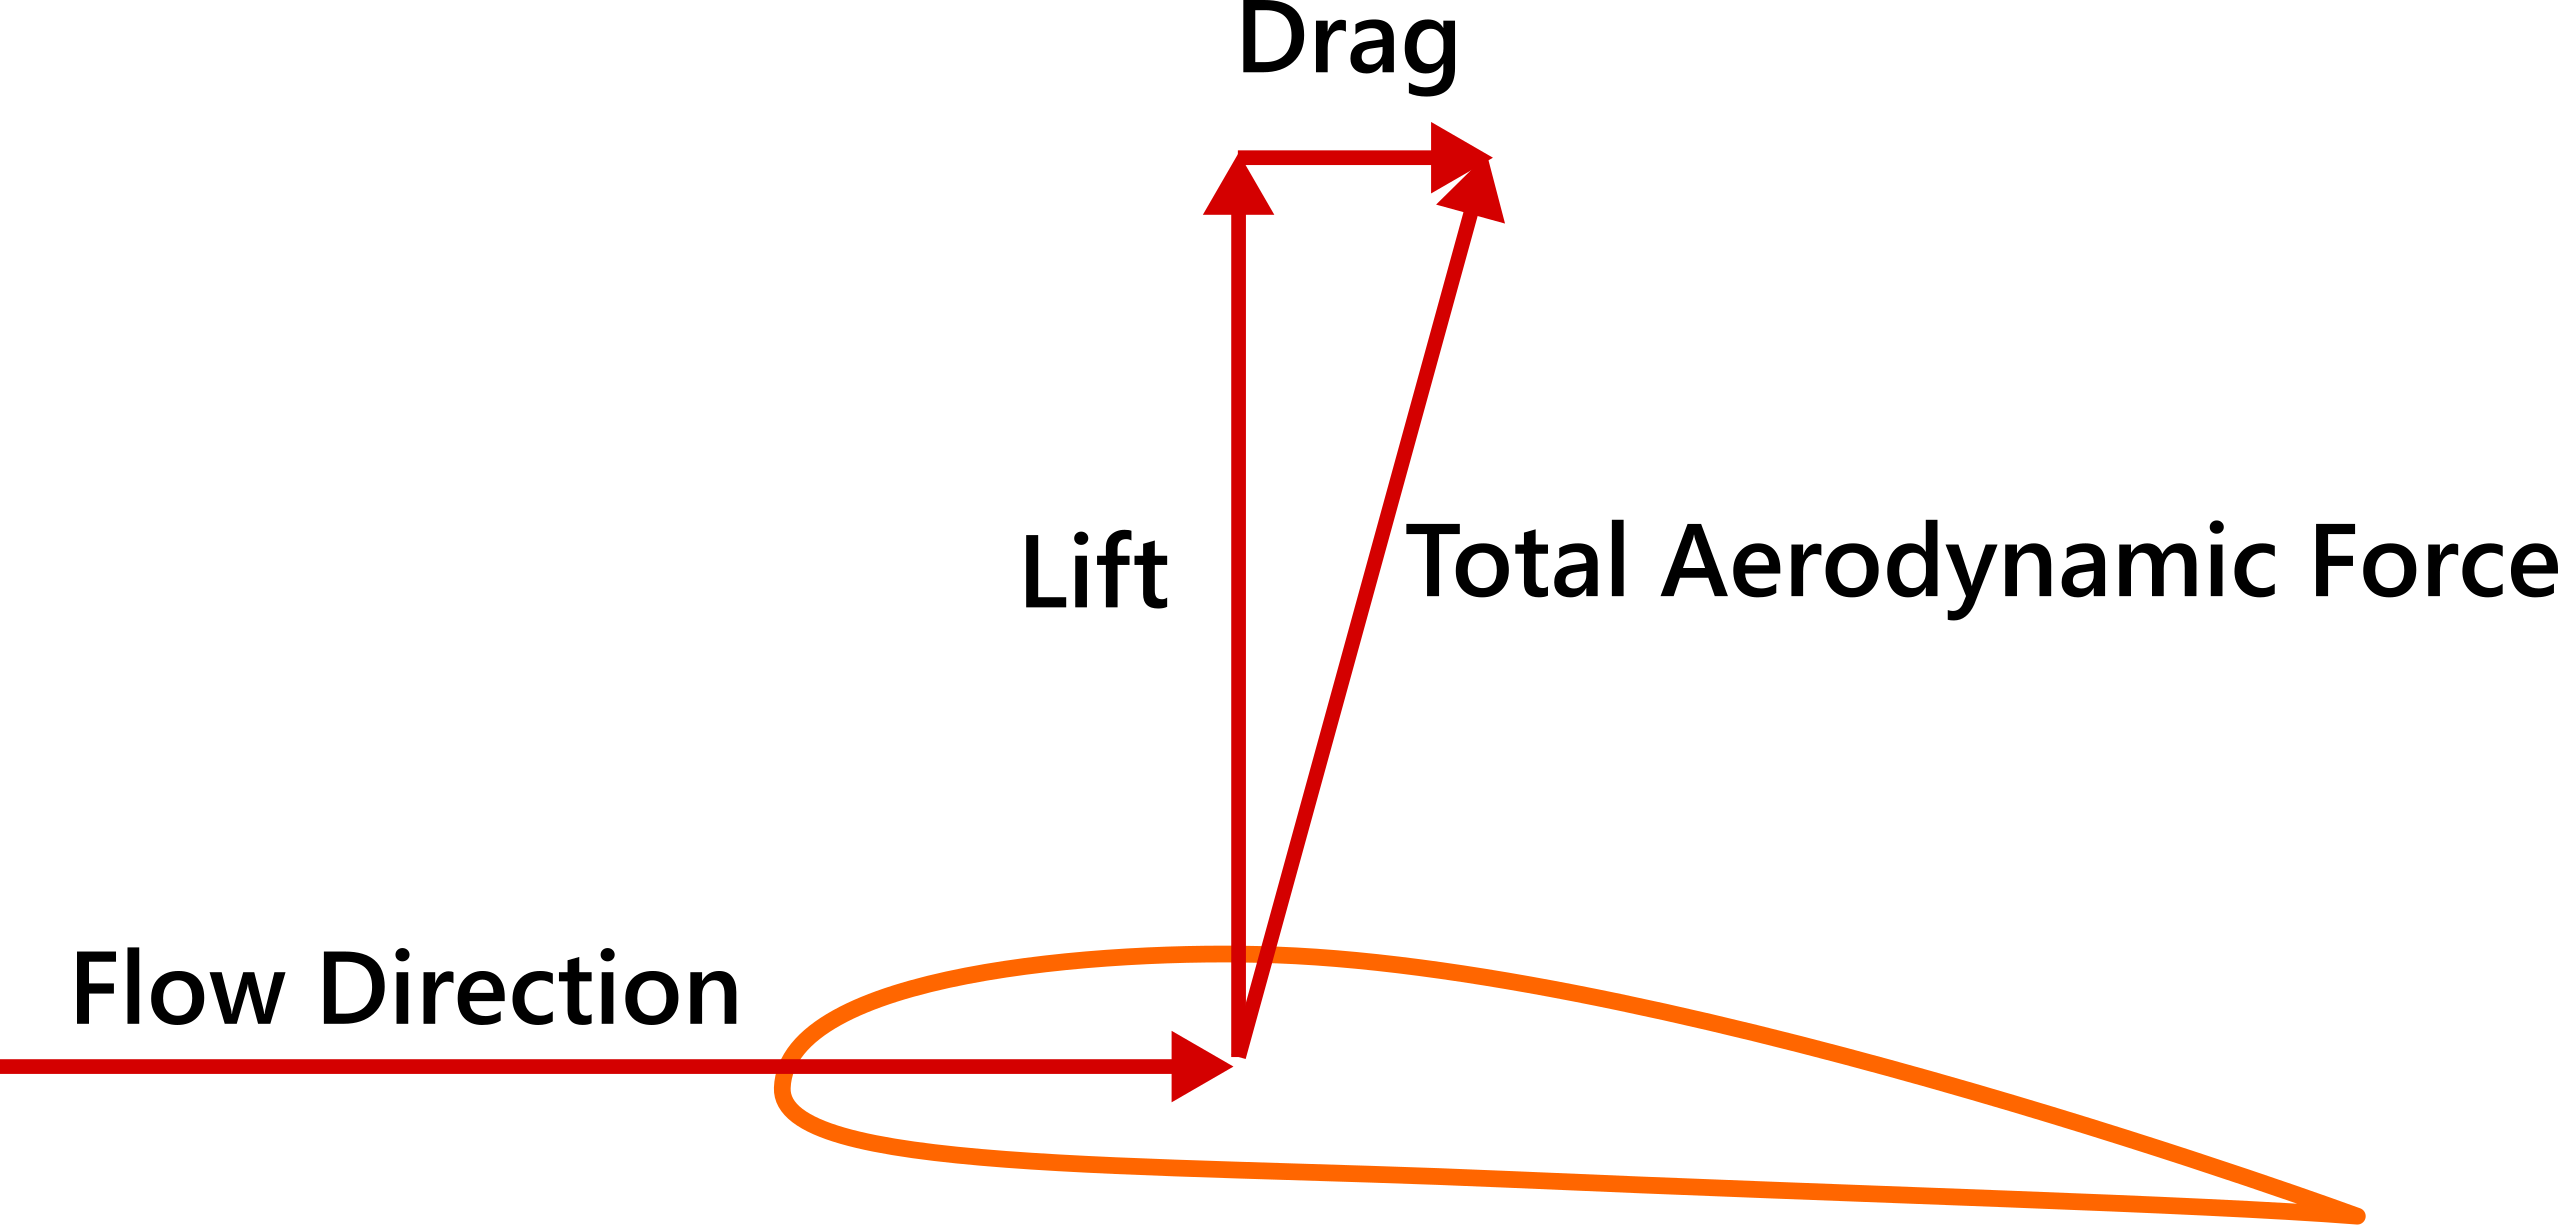
\includegraphics[width=0.4\textwidth]{liftdrag.png}
    \caption{An illustration of how the flow of air over an airfoil generate Lift and Drag. \cite{liftdragpng}}
    \label{fig:liftdrag}
\end{figure}

The lift force can further be broken down into several parts, but aerodynamics is a complicated field, and for the purposes of this thesis we only consider the following:
Lift due to camber (the non symmetry of the wing in the airstream), lift due to angle of attack (the angle which the incoming air makes with the wing) and lift due to control surface deflection.

\subsubsection{Propeller lift}
The force from propellers will be dealt with in greater detail further into this thesis.
But as an introduction they can be thought of as wings moving through the air, only in a rotational matter instead of straight on. 
As they move through the air lift is generated in a similair fashion to normal wings, but since the propeller is mounted at a right angle to the wings the lift force propels the aircraft forward.
The air a propeller displaces is called a wake and will be treated as a separate airflow from the aircraft moving through the air.


%\begin{itemize}
%        \item Bernoulli Equation, center of Pressure, etc
%        \item Basic plate theory
%        \item Aerodynamic center    
%        \item Aerodynamic forces and Moments
%        \begin{itemize}
%            \item Lift, and moment, due to camber
%            \item Lift due to angle of attack
%            \item Drag
%            \item Forces/Moments due to airflow over Ailerons and Elevators
%            \item Forces and Moments due to sideslip and roll
%            \item Forces/Moment due to roll rate, pitch rate and yaw rate
%        \end{itemize}
%        \item Propeller efficiency, airspeed, wake velocity
%    \end{itemize}

\section{Mathematical Model of EcoSoar}
To develop a control system first a simulator needs to be developed, and so the aircraft has to be mathematically modeled.
To not make the simulator too time consuming to develop nor to complex a few assumptions will be made:
\section{Assumptions}

\begin{itemize}
    \item There is no external wind and so $v_{\infty}$ is replaced with $v$ which is the aircrafts velocity through the air.

    \item All forces operate on points in the $x-y$ plane, i.e. no offset in the $z$-direction (with the notable exception of the winglet forces). Forces may still have a $z$-component though.

    \item The propeller wake is unaffected by aircraft velocity, i.e. only determined by propeller speed.

    \item Airflow outside of wake is only determined by aircraft velocity.

    \item The aerodynamic centre (a.c.) is static and does not move with changes in speed and pressure. The moment around it, however, will vary and thus account for the effects of the a.c. movement.

    \item Airflow speed in wake is proportional to propeller rotational speed, $v_w = b_w \omega_i$, where $b_w$ is a constant.

    \item The principal moments axis align with the symmetry plane; only diagonal elements in the inertia matrix aligned with the body frame coordinate axis.

    \item Roll moment due to sideslip angle, negligible due to lack of tail with verical offset from c.g.

    \item Yawing moment due to roll rate is negligible due to the lack of a tail.

    \item Forces and moments due to acceleration are not explicitly calculated; they are already included in  dynamic model since it is based on forces.

\end{itemize}

%\section{Coordinate system}
NED: North East Down.
$x$-axis is essentially the forward direction of the airplane in normal flying mode.
$z$-axis is pointed downwards.
$y$-axis is along the right wing.


\subsection{Aircraft force diagram}
The aircraft in question is the EcoSoar; a flying wing.
It has two control surfaces, one on each wing called elevons.
In front of each wing a motor and propeller is mounted providing thrust.
The motors also supply an airflow over the control surfaces when the aircraft is not moving through the air.


\begin{figure}[h]
    \center
    \begin{tikzpicture}
    \begin{tikzpicture}
    \begin{scope}[shift={(6,2.4)}]
    % Coord sys.
    \begin{scope}[shift={(1.2,-0.1)}]
        \draw[thick, ->] (-6,2) -- (-6,2.5) node[anchor=south east]{$x$};
        \draw[thick, ->] (-6,2) -- (-5.5,2) node[anchor=south west]{$y$};
        \draw[] (-6,2) circle (0.15cm);
        \draw[] (-6.1,1.9) -- (-5.9,2.1);
        \draw[] (-6.1, 2.1) -- (-5.9,1.9);
        \node[] at (-6.3,1.9) {$z$};
    \end{scope}

    % main body
    \draw (0,0) rectangle (1,2);
    % left wing
    \draw (0,2) -- (-5,0) -- (-5,-1) -- (0,0);
    % right wing
    \draw (1,2) -- (6,0) -- (6,-1) -- (1,0);
    % winglets, left and right
    \draw[very thick] (6,0) -- (6,-1);
    \draw[very thick] (-5,0) -- (-5,-1);

    % wingspan
    \draw[<->, thin] (-5,-2.2) -- (6, -2.2);
    \draw[dotted] (-5,-1) -- (-5, -2.5);
    \draw[dotted] (6, -1) -- (6, -2.5);
    \node at (0.5,-2.4) {$b$};

    % right Winglet forces
    \draw[fill=black] (6,-0.5) circle (0.05cm) ;
    \draw[->, thick] (6,-0.5) -- (6.5, -0.5);
    \node[] at (6.7,-0.8) {$L_{W_R}$};
    \draw[dotted] (6,-0.5) -- (7.2,-0.5);
    \draw[very thin, <->] (6.7,-0.5) -- (6.7, 1.4);
    \node[] at (7, 0.4) {$x_W$};

    \draw[->, thick] (6,-0.5) -- (6, -1.5);
    \node[] at (6.5,-1.5) {$D_{W_R}$};

    %left and right flaps
    %\draw (-4.4,-0.88) circle (0.1cm);
    %\draw (-1, -0.2) circle (0.1cm);
    \draw (-4.4, -0.88) -- (-4.4, -0.5) -- (-1, 0.25) -- (-1, -0.2);
    \draw (5.4, -0.88) --  (5.4, -0.5) -- (2, 0.25) -- (2,-0.2);

    % left and right propellers
    \draw[thick, ->] (-2.5,1) -- (-2.5,2) node[anchor=south east]{$T_L$};
    \draw[thick, ->] (3.5,1) -- (3.5, 2) node[anchor=south west]{$T_R$};

    % prop distance to cg
    \draw[<->] (-2.5, 2.5) -- (0.5, 2.5);
    \node[] at (-1, 2.7) {$y_T$};
    \draw[dotted] (3.5,2) -- (4.5,2);
    \draw[<->] (4.5,2) -- (4.5,1.4);
    \node[] at (4.8, 1.7) {$x_T$};

    % propeller cone. Left then Right
    \draw[dotted] (-3,2) -- (-3,-1);
    \draw[dotted] (-2,2) -- (-2,-1);
    \draw[dotted] (4,2) -- (4,-1);
    \draw[dotted] (3,2) -- (3,-1);

    % Propeller cone width
    \draw[<->] (4,-1) -- (3,-1);
    \node[] at (3.5, -1.2) {$y_w$};

    % Surface area aileron
    \node[] at (-2.5, -0.3) {$S_{a_w}$};
    \node[] at (-3.6, -0.53) {$S_a$};
    \node[] at (-1.6, -0.1) {$S_a$};

    % Wind surface areas
    \node[] at (2,0.8) {$S_w$};
    \node[] at (5,0) {$S_w$};
    \node[] at (3.35,0.85) {$S_{w_w}$};

    % Lift force, left
    \draw (-2.2, 0.4) circle (0.2cm);
    \draw[fill=black] (-2.2, 0.4) circle (0.025cm);
    \node[] at (-1.7, 0.4) {$L_L$};

    % Lift force, right
    \draw (3.2, 0.4) circle (0.2cm);
    \draw[fill=black] (3.2, 0.4) circle (0.025cm);
    \draw[dotted] (3.2, 0.4) -- (6.5,0.4);
    \node[] at (2.7, 0.4) {$L_R$};

    % Drag force, right
    \draw[->] (3.2,0.4) -- (3.2, -0.3);
    \node[] at (3.5,-0.3) {$D_R$};

    % Lift force distance
    \draw[<->] (0.5, -0.7) -- (3.2, -0.7);
    \node[] at (2, -0.5) {$y_{ac}$};
    % Right x distance
    \draw[<->] (6.2,1.4) -- (6.2, 0.4);
    \node[] at (5.8, 0.9) {$x_{ac}$};

    % Aileron force
    \draw (-2.5, -0.9) circle (0.2cm);
    \draw[] (-2.35, -0.75) -- (-2.65,-1.05);
    \draw[] (-2.65, -0.75) -- (-2.35, -1.05);
    %\node[] at (-2.4, -1.3) {$F_L$, $F_{L_T}$};
    \node[] at (-1.5, -1.0) {$F_L$, $F_{L_T}$};
    \draw[dotted] (-2.5, -0.9) -- (-5.5, -0.9);
    % Aileron drag
    \draw[->, thick] (-2.5, -0.9) -- (-2.5, -1.5);
    \node[] at (-1.4, -1.4) {$D_{a_L}$, $D_{a_{L,T}}$};

    % Distance flap force
    \draw[<->] (0.5,-1.8) -- (-2.5, -1.8);
    \node[] at (-1, -2) {$y_f$};
    \draw[<->] (-5.3, 1.4) -- (-5.3, -0.9);
    \node[] at (-5.6, 0.2) {$x_f$};

    % Center of Grav.
    \draw[fill=black] (0.5, 1.4) circle (0.1cm);
    \draw[dotted] (0.5,1.4) -- (0.5,-2);
    \draw[dotted] (0.5,1.4) -- (7.1,1.4);
    \draw[dotted] (0.5,1.4) -- (-5.5,1.4);
    \node[] at (0.55, 1.1) {c.g.};


    %mark 0,0
    %\draw (0,0) circle (0.1cm);

\end{scope}
\end{tikzpicture}
    \end{tikzpicture}
    \caption{Drawing of the EcoSoar, its propellers with wake and its control surfaces in body frame.}
    \label{airplane}
\end{figure}

The elevon forces, $F_L$, $F_{L_T}$, $D_{a_{L}}$ and $D_{a_{L,T}}$, have only been marked on the left wing, but exist symmetrically on the right wing with index $R$ instead of $L$.
The same is true for the drag force, $D_R$ and the winglet forces, $L_{W_R}$ and $D_{W_R}$, existing symmetrically on the left side.
$F_L$ is the force due to elevon deflection over surface area $S_a$, and $F_{L_T}$ is the force due to elevon deflection over $S_{a_w}$; the surface in the wake of the propeller.
Similarly for the drag, $D_{\alpha_L}$, $D_{\alpha_{L,T}}$, forces.
We also split the wing area into two sections: $S_w$ for the wing area outside the wake, and $S_{w_w}$ for the wing area in the wake.
The thrust forces, $T_i$, are assumed to act at the arrow end of the vector due to the offset in $x$ created by the motor and drive shaft.
The lift forces, $L_L$ and $L_R$, are functions of airflow over wing outside of wake and in the wake, which in turn are functions of aircraft velocity, propeller speed, angle of attack, air density, wing shape, etc.



\subsubsection{Aerodynamic Lift force}

The lift force of a wing depends on several factors.
Mainly: geometrical shape, dynamic pressure and angle of attack.\cite{aerodynamics}
The bigger the wing the more lift.
The faster air flows the more lift.
The further away from hitting the wing straight on, usually more lift.

Important note: Lift is defined as the \textbf{Aerodynamic force component perpendicular to the incoming airflow.} This means that, for example, the lift force labeled in figure \ref {airplane} as \textbf{$L_L$ is not the aerodynamic lift but rather the lift force in body frame.} The same argument applies to the drag forces.

Aerodynamic lift is usually modeled as\cite{nelson}\cite{aerodynamics}:
\begin{equation}
    L = Q  C_L S
\end{equation}
where $S$ is a reference surface area of the wing and $Q$ is the dynamic pressure:
\begin{equation}
    Q = \frac{1}{2} \rho v^2
\end{equation}
$\rho$ is the density of air and $v$ the velocity of the air hitting the wing.
$C_L$ is the coefficient of lift, a function of the angle of attack.
This coefficient is not linear. Empirical studies\cite{aoa180}\cite{aoa180-2} have found functions similair to the one in figure \ref{clalpha}.
\begin{figure}[h]
    \center
    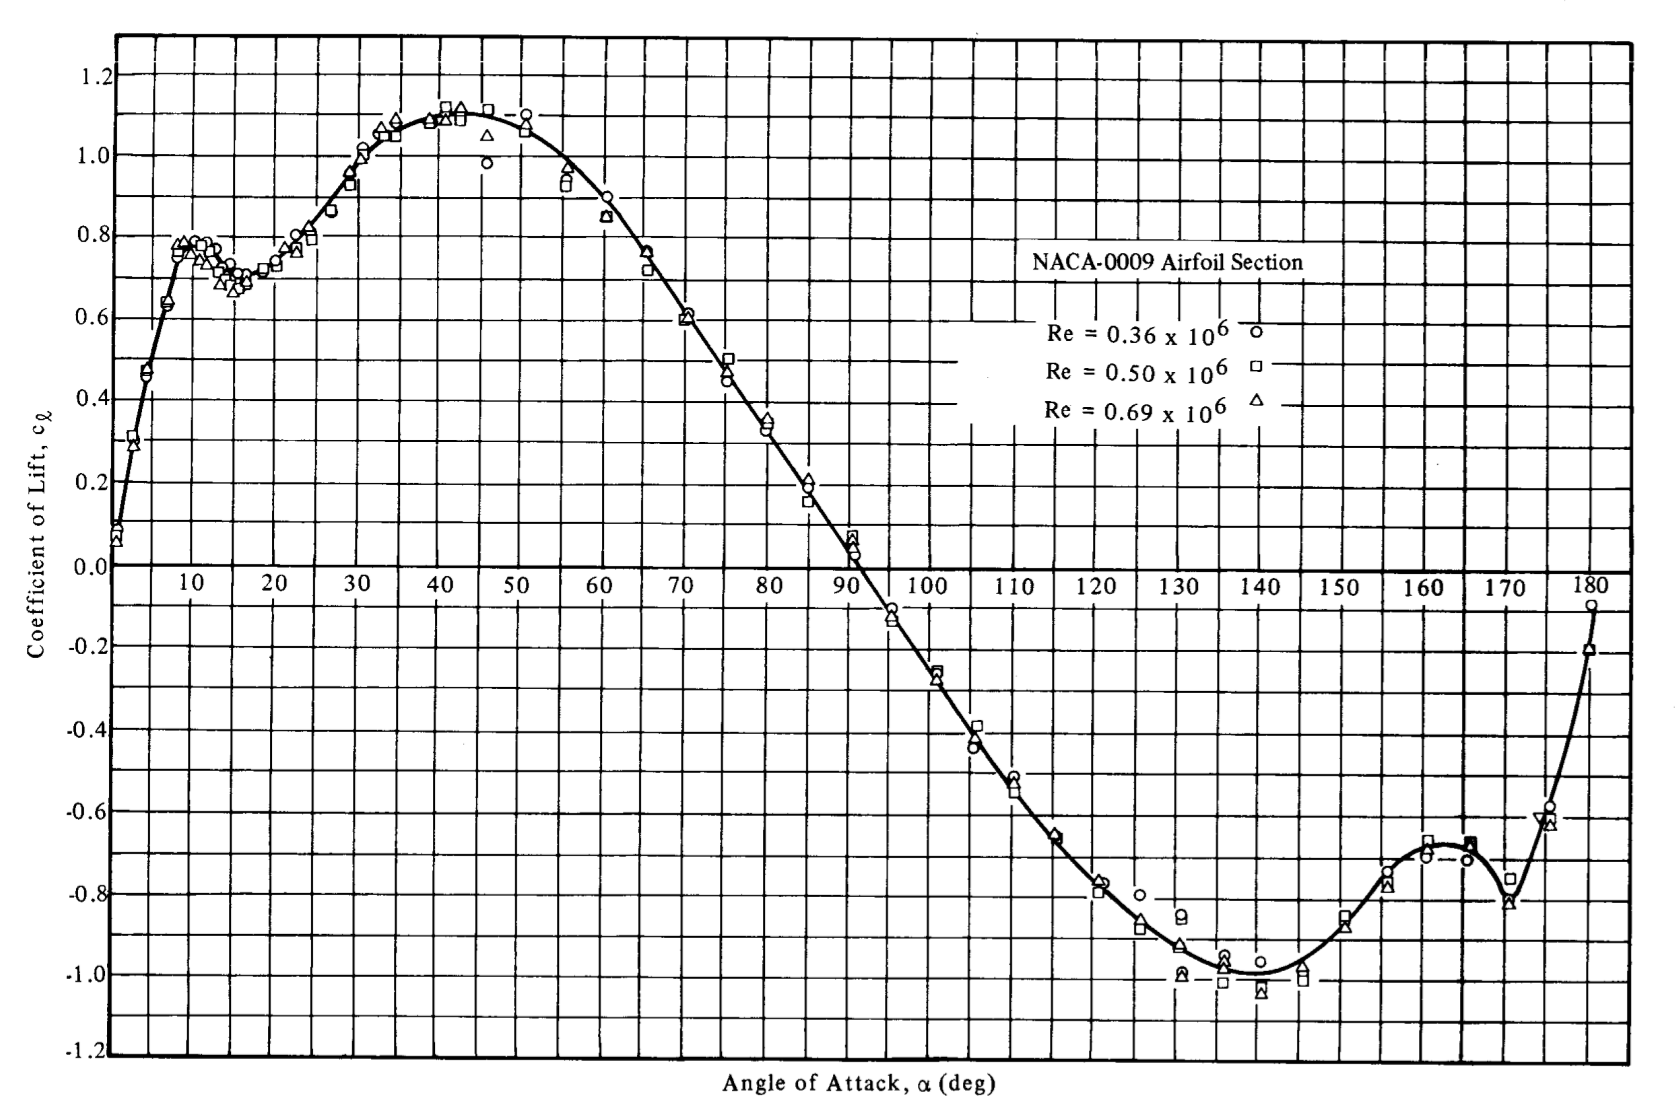
\includegraphics[scale=0.15]{aoa_80s.png}
    \caption{Coefficient of lift for a symmetrical wing vs angle of attack for the entire 180 degree rotation of the wing. The function is periodic.}
    \label{clalpha}
\end{figure}

The angle of attack, $\alpha$, is formally the angle at which the air is hitting the wing relative the body frame x-z axis.
If air is aligned with the $x$-axis $\alpha$ is zero, and if aligned with the $z$-axis $\alpha$ is 90.
(The airflow will obviously be in the negative axis direction since the airplane is flying in the positive direction and hitting the air).
Thus, if we assume no wind the angle of attack is only dependent on the aircraft velocity $\bar{v}$.
Normally this is modeled as:
\begin{equation}
    \alpha = tan^{-1}(\frac{v_z}{v_x})
    \label{eq:aoa}
\end{equation}
but in our case the velocity may have any direction in the $x$-$z$ plane, and is not limited to the right half plane.
The polar coordinates for vector $\bar{v}$ in the figure below, figure \ref{polar}, are:
\begin{equation}\begin{split}
    v_x =& \, r \, cos(\alpha) \\
    v_y =& \, r \, sin(\alpha) \\
    r =& \sqrt{v_x^2 + v_z^2}
    \label{eq:polar}
\end{split}\end{equation}
where $\alpha$ is in the interval $[-\pi,\pi]$.

\begin{figure}[h]
    \center
    \begin{tikzpicture}
    
    \draw[->] (-2,0) -- (2,0); % x-axis
    \node[] (x) at (2,-0.2) {$v_x$};
    \draw [->](0,-1) -- (0,2); % y-axis
    \node[] (y) at (0.3,2) {$v_z$};

    % Vector
    \draw[->, thick] (0:0) -- (90+45:1.5);
    \node[] at (90+45:1.7) {$\bar{v}$};

    % help lines
    \draw[dotted] (-1.05,0) -- (90+45:1.5);
    \draw[dotted] (0,1.05) -- (90+45:1.5);

    % angle
    \draw[->] (0.3,0) arc(0:45+90:0.3);
    \node[] at (0.3,0.4) {$\alpha$};
\end{tikzpicture}
    \caption{Velocity vector $\bar{v}$ in polar coordinates.}
    \label{polar}
\end{figure}

\subsubsection{Aerodynamic drag}
Similarly to aerodynamic lift the wing will also have an aerodynamic drag force, but parallel to the incoming flow and not perpendicular as lift.
The drag is also modeled like so:
\begin{equation}
    D = Q C_D S
\end{equation}
where the coefficient of drag, $C_D$, can also be experimentally obtained as in figure \ref{drag}.

\begin{figure}[h]
    \center
    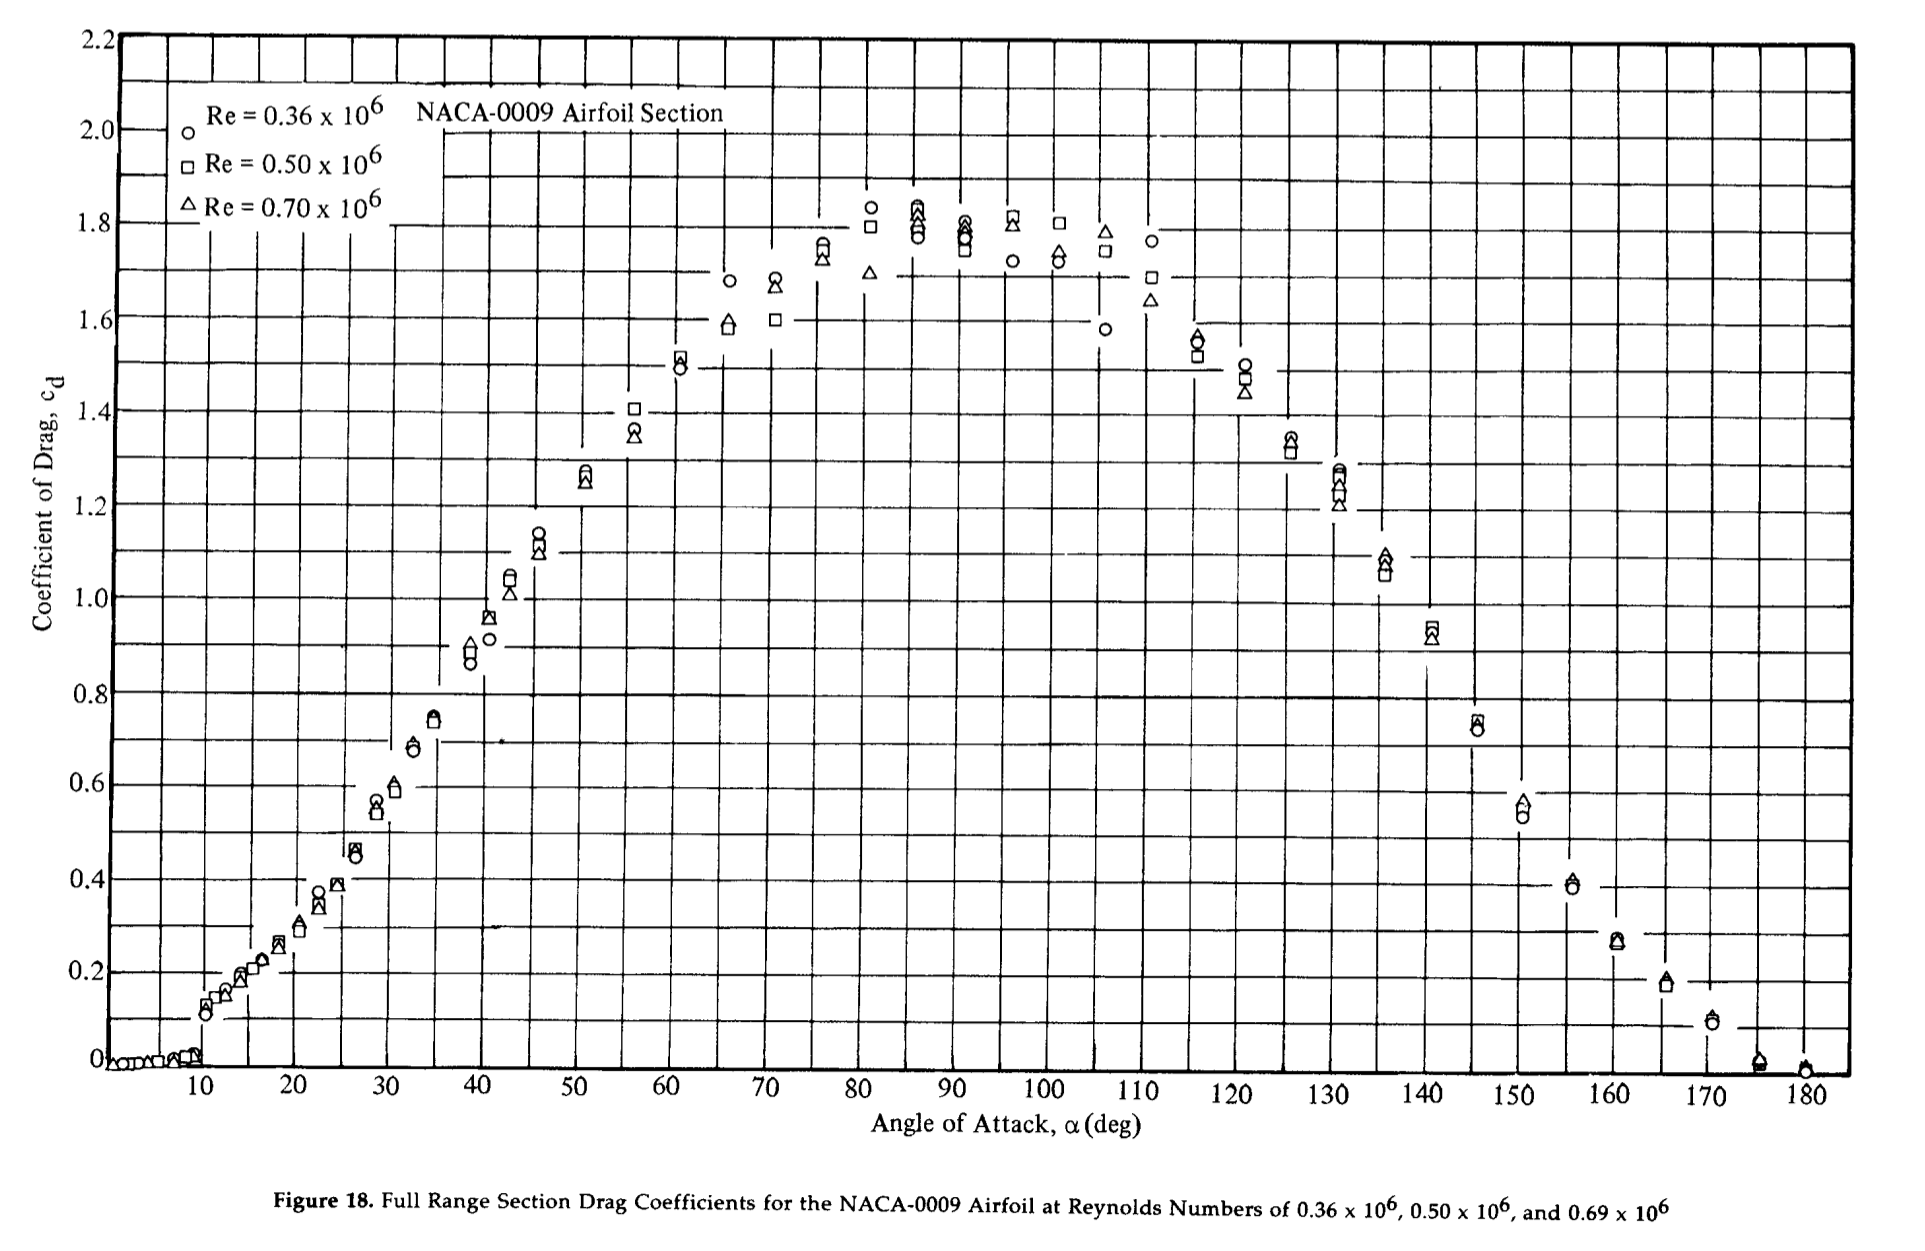
\includegraphics[scale=0.15]{drag180.png}
    \caption{Coefficient of drag for a symmetrical wing vs angle of attack for the entire 180 degree rotation of the wing.}
    \label{drag}
\end{figure}


\subsubsection{Lift and drag in body frame}

Since the aerodynamic lift and drag forces are relative the incoming airflow, i.e. functions of the angle of attack, $\alpha$, the body frame Lift and Drag have to transformed:
\begin{equation}\begin{split}
    L_i &= cos(\alpha) L + sin(\alpha) D \\
    D_i &= -sin(\alpha) L + cos(\alpha) D
    \label{LDbodyframe}
\end{split}\end{equation}
Note that the above forces are in the direction labeled in figure \ref{airplane} and not necessarily in the positive axis they act in.
From equation \ref{eq:polar} we see that
\begin{equation}\begin{split}
    v_x =& \, r \, cos(\alpha) \Rightarrow cos(\alpha) = \frac{v_x}{\sqrt{v_x^2 + v_z^2}} \\
    v_z =& \, r \, sin(\alpha) \Rightarrow sin(\alpha) = \frac{v_z}{\sqrt{v_x^2 + v_z^2}}
\end{split}\end{equation}
If we substitute in expressions for aerodynamic lift and drag we obtain:
\begin{equation}\begin{split}
    L_i =&  \frac{v_x}{\sqrt{v_x^2 + v_z^2}} Q C_L S +
            \frac{v_z}{\sqrt{v_x^2 + v_z^2}} Q C_D S \\
    D_i =& -\frac{v_z}{\sqrt{v_x^2 + v_z^2}} Q C_L S +
            \frac{v_x}{\sqrt{v_x^2 + v_z^2}} Q C_D S \\          
\end{split}\end{equation}
which simplify into:
\begin{equation}\begin{split}
    L_i =& 
     S \frac{1}{2} \rho v^2 \left( \frac{C_L v_x + C_D v_z}{\sqrt{v_x^2 + v_z^2}} \right) \\
     %
    D_i =& 
     S \frac{1}{2} \rho v^2 \left( \frac{-C_L v_z + C_D v_x}{\sqrt{v_x^2 + v_z^2}} \right)
     \label{liftdragbody}
\end{split}\end{equation}
where $v = \sqrt{v_x^2 + v_y^2 + v_z^2}$.


\subsection{Moment due to force}

Any force not acting at the center of gravity will produce a moment around c.g.
The moment of a force is:
\begin{equation}
    \bar{M} = \bar{r} \times \bar{F}
\end{equation}
With our assumptions the above equation can be written as:
\begin{equation}
    \bar{M} = (r_x, r_y, 0) \times (F_x, F_y, F_z) = 
    \left[ \begin{matrix}
    F_z r_y \\
    -F_z r_x \\
    F_y r_x - F_x r_y \end{matrix} \right]
\end{equation}

\subsubsection{Pitching moment}
Lift due to camber on a wing acts at ~50\% of the cord line.
Lift due to angle of attack acts at roughly 25\% of the cord line.\cite{aerodynamics}
This makes the force acting point, center of pressure, move along the cord line when angle of attack and aircraft velocity changes.
A common simplification is to choose the aerodynamic center, a.c., as the point at which Lift acts.
It can be shown that placing the a.c. at the 25\% cord position 
makes the moment generated vary little as angle of attack changes, yielding simpler equations.
The pitching moment due to lift can now be expressed as:
\begin{equation}
    \tau_{y,lift} = \sum_{j \in [w, w_w]}
    C_{m,y,l} Q S_j l +  \cancelto{0}{\sum_{j \in [w, w_w]}
    C_{m,y,l,\alpha} Q S_j l \alpha}
\end{equation}
where $l$ is the characteristic length of the wing, usually taken as the mean cord for pitching moments and the wingspan for rolling and yawing moments.

\subsection{Equations of motion}

The equations of motion can be split into three parts: one part due to gravity, one part due to the rigid body frame being an accelerated reference frame, and one part due to aerodynamic forces.
These forces depend on the aircrafts attitude and will be expressed in terms of it.

\subsubsection{Attitude}
The attitude is represented by a quaternion:
\begin{equation}
\bar{q} = [q_0, q_1, q_2, q_3]^T
\end{equation}
Any vector, $\bar{r}_w$, in world frame can be represented in the body frame by the conversion:
\begin{equation}
    \bar{r}_b = \bar{q} \bar{r}_w \bar{q^*}
\end{equation}

\subsubsection{Gravity}
In the case of gravity, $\left[\begin{smallmatrix}0\\0\\mg\end{smallmatrix}\right]_w$, the force, $m \bar{g}$, becomes
\begin{equation}
m \dot{\bar{v}}_b = \left[ \begin{matrix}
    2 (\bar{q_1} \bar{q_3} + \bar{q_0} \bar{q_2})  \\
    2 (\bar{q_2} \bar{q_3} - \bar{q_0} \bar{q_1})  \\
    (\bar{q_0}^2 - \bar{q_1}^2 - \bar{q_2}^2 + \bar{q_3}^2) 
    \end{matrix} \right] m g
\end{equation}
Gravity acts in the center of gravity and creates no moment.
Since gravity is in world frame and we want to express it in body frame we need to conjugate the quaternion.

\subsubsection{Forces and moments due to accelerated body reference frame}

In the case of a rigid body with inertia matrix $I$, velocity $\bar{v}$ and angular velocity $\bar{\omega}$ relative a fixed frame we have the moment equation:
\begin{equation}
    I \dot{\bar{\omega}} = \bar{\tau} - \bar{\omega} \times
    I \bar{\omega}
\end{equation}
where $\tau$ is the external torque acting on the body.

Similarly, if we include the coriolis force we obtain the forces in our body frame:
\begin{equation}
    \bar{F} = \bar{F}_{e} 
    + 2 m \, \bar{\omega} \times \bar{v}
\end{equation}
where $\bar{F_e}$ is the external forces acting on the body.
No other inertial forces are of interest;
the linear accelleration is irrelevant since we are not flying inside a linearly accellerating frame, and the other two depend on rotation around a non principal axis.

In our case, with assumptions made, the above equations simplify to:

\begin{equation}
\left[
\begin{matrix}
    \dot{\bar{v}} \\
    \dot{\bar{\omega}}
\end{matrix} \right]
=
\left[
\begin{matrix}
    \dot{v_x} \\
    \dot{v_y} \\
    \dot{v_z} \\
    \dot{\omega_x} \\ 
    \dot{\omega_y} \\
    \dot{\omega_z}
\end{matrix} \right] 
=
- \left[ \begin{matrix}
2 ( v_z \omega_y - v_y \omega_z )\\
2 ( v_x \omega_z - v_z \omega_x )\\
2 ( v_y \omega_x - v_x \omega_y )\\
\frac{1}{I_x} (I_z - I_y) \omega_y \omega_z \\
\frac{1}{I_y} (I_x - I_z) \omega_x \omega_z \\
\frac{1}{I_z} (I_y - I_x) \omega_x \omega_y 
\end{matrix} \right]
+ \verb!external forces and moments!
\end{equation}


\subsubsection{elevons}
Aileron forces are modeled similarly to lift, as well, but with an extra term, $\delta_i$, for the deflection degree in radians:
\begin{equation}
    F_i = C_{L_\delta} \sum_{j \in [a, a_w]}  Q_{j,i} S_j \delta_i
\end{equation}
and similairly the drag created by the ailerons:
\begin{equation}
    D_{\alpha_i} = C_{D_\delta} \sum_{j \in [a, a_w]}  Q_{j,i} S_j \delta_i
\end{equation}
The aileron lift, and drag, coefficient is assumed to be static over all angle of attacks since they will be in the wake of the wing, and the lift and drag are linear in the region of angles the ailerons can deflect.


\subsection{Winglets, forces and moments due to sideslip}
The aircraft considered here has no tail nor separate body (as the body is part of the wing).
The only surfaces providing relevant forces due to sideslip are the winglets.
The winglets each have an area $S_W$ and are flat plate wings which will generate aerodynamic lift and drag forces due to $\beta$ providing an angle of attack in their reference frame.
$\beta$ can be, similarly to $\alpha$, be expressed in polar coordinates:
\begin{equation}\begin{split}
    v_x =& \, r \, cos(\beta) \\
    v_y =& \, r \, sin(\beta) \\
    r =& \sqrt{v_x^2 + v_y^2}
\end{split}.
\end{equation}
Note that $\beta$ is in the $x$-$y$ plane and not $x$-$z$ plane as in the case for $\alpha$.
$\beta$ can be described as the horizontal incoming angle relative the airfraft body frame and since the winglets are vertical this will act as their angle of attack.


The aerodynamic forces, $L_\beta$ and $D_\beta$, from the winglets convert into body forces, as in figure \ref{airplane}, similarly to lift and drag from the main wings:
\begin{equation}\begin{split}
L_{W_i} &= cos(\beta) L_\beta +  sin(\beta)D_\beta \\
D_{W_i} & = -sin(\beta) L_\beta + cos(\beta) D_\beta
\end{split}\end{equation}
where
\begin{equation}\begin{split}
L_\beta &= Q C_{L_\beta} S_W \\
D_\beta & = Q C_{D_\beta} S_W
\end{split}\end{equation}
and $C_{k_\beta}$ are the lift and drag coefficients for each winglet, here assumed to be flat plates.
$v_z$ can be assumed to be negligible in the following equations since the physics from the main wings will dominate the effects due to $v_z$.
If we assume $v_z$ to be negligible then we obtain:
\begin{equation}\begin{split}
L_{W_i} &= 
    \frac{\rho v S_W}{2}  \left( C_{L_\beta} v_x + v_y C_{D_\beta} \right) \\
%
D_{W_i} &= 
    \frac{\rho v S_W}{2 }  \left(-v_y C_{L_\beta} + v_x C_{D_\beta} \right)
\end{split} .
\end{equation}
If the sideslip angle, $\beta$, is small (which implies $v_y$ small) the lift and drag coefficients can be approximated as 
\begin{equation}\begin{split}
    C_{L_\beta} \approx& \frac{d C_{L_\beta}}{d \beta} \big\vert_{\beta=0} \, \beta \\
    C_{D_\beta} \approx& 0
\end{split}\end{equation}
where the Lift coefficient is assumed linear with respect to $\beta$, which makes sense looking at figure \ref{clalpha}.
Similarly, Drag for a flat plate is roughly zero around zero angle of attack.
This results in:
\begin{equation}\begin{split}
L_{W_i} &\approx 
    \frac{\rho v S_W}{2} \frac{d C_{L_\beta}}{d \beta} \big\vert_{\beta=0} \, \beta \, v_x  \\
%
D_{W_i} &\approx 0
\end{split}\end{equation}
This gives us, in body frame, one restoring force from each winglet roughly proportional to the forward velocity squared of the aircraft and the sideslip angle..
The forces have the same magnitude and direction on both sides of the aircraft.



\subsubsection{Restoring moment}

$D_{W_i}$ are symmetrical on both sides and only create an acceleration in $y$.
They do not generate any moment.
$L_{W_i}$, however, act asymmetrically around c.g.~and do generate a torque (note that the force $L_{W_R}$ generates a negative torque around $z$ in our coordinate system):
\begin{equation}
    M_z = L_{W_L} x_W + L_{W_R} x_W = - \rho v S_W \frac{d C_{L_\beta}}{d \beta} \big\vert_{\beta=0} \, \beta \, v_x x_W
\end{equation}

\subsubsection{Non linear forces and moments}
If we do not make the assumption that $\beta$ is small we instead get the equations:
\begin{equation}\begin{split}
    M_z =& - \, x_W \rho v S_W  \left( C_{L_\beta}(\beta) v_x + v_y C_{D_\beta}(\beta) \right) \\
    D_{W} =& \rho v S_W \left(-v_y C_{L_\beta}(\beta) + v_x C_{D_\beta}(\beta) \right)
\end{split}\end{equation}
where $D_W = D_{W_L} + D_{W_R}$, and the coefficients of lift and drag are as shown in the figures \ref{clalpha} and \ref{drag}, but functions of $\beta$ instead of $\alpha$ as $\beta$ becomes the effective angle of attack in the winglets reference frame.



\subsubsection{Rolling moment due to sideslip}

The center of the winglet is slightly offset in the $z$-direction from the c.g. by distance $z_W$. 
Given the forces $L_{W_i}$ the rolling moment due to sideslip, $M_x$, is simply
\begin{equation}
    M_x = z_W (L_{W_L} + L_{W_R})
\end{equation}



\subsection{Propeller Thrust}
Thrust will be modeled as
\begin{equation}
    T_i = K_T \omega_i^2
\end{equation}
where $K_T$ is the thrust coefficient of the propeller and $\omega_i$ the rotational speed of the propeller.

Behind the propellers an area of airflow is generated, called a wake.
Given a propeller diameter of $d_P$, pushing air through at a rate of $v_w$ the volume of air being moved by the propeller during time $t$ is:
\begin{equation}
	V_{air} = \int_0^t \frac{d}{2} \pi^2 v_w dt \,.
\end{equation}
The air has density $\rho$ converting the volume into mass:
\begin{equation}
	m_{air} = \rho \, m_{air}
\end{equation}
If we assume the air to be stationary in front of the propeller and the aircraft standing still the change in momentum in the air is:
\begin{equation}
	\Delta p = m_{air} v_{air} = \rho \frac{d \pi^2}{2} v_w^2 t
\end{equation}
Force due to change in momentum is:
\begin{equation}
	F t = \Delta p \Rightarrow F = \frac{\Delta p}{t}
\end{equation}
giving us:
\begin{equation}
	F = \rho  \frac{d \pi^2}{2} v_w^2 \, .
\end{equation}
By combining all parameters into one coefficient $K_v$, the following equation is obtained:
\begin{equation}
	F = K_v  v_w^2 \, .
\end{equation}

If we instead look at the lift generated by the propeller blades we can find the thrust as a function of propeller rotation speed.
Assuming the aircraft has no speed and there is no wind we can model the lift from one propeller blade as:
\begin{equation}
	L_i = \int_0^{\frac{d}{2}} \frac{\rho}{2} (\omega_i r)^2 C_L(pitch) dr
\end{equation}
If we also assume a constant pitch along the diameter of the propeller blade the above integral simplifies into:
\begin{equation}
	L_i = \frac{\rho d^3}{48} C_L(pitch) \omega_i^2
\end{equation}
and thus with $n$ blades we find the total lift, i.e. thrust:
\begin{equation}
	T_i = L = \sum_{i \in [1,n]} L_i = n L_i
\end{equation}

By comparing the equation for thrust due to rotation speed and thrust due to airflow we conclude that:
\begin{equation} \begin{split}
	K_v v_w^2 =& n \frac{\rho d^3}{48} C_L(pitch) \omega_i^2 \Rightarrow \\
	& v_w = b_w \omega_i
\end{split}\end{equation}
and so the assumption that airflow in the wake is proportional to the propeller angular speed holds.



\subsection{Restoring moment due to roll rate}
\label{sec:restmomroll}
If we assume that $v_y$ is negligible then the Lift and Drag forces in body fram simplify into:
\begin{equation}\begin{split}
    L_i =& 
     S \frac{1}{2} \rho v^2 \left( \frac{C_L v_x + C_D v_z}{\sqrt{v_x^2 + v_z^2}} \right) = 
      S \frac{1}{2} \rho \sqrt{v_x^2 + v_z^2} \left(C_L v_x + C_D v_z \right)\\
     %
    D_i =& 
     S \frac{1}{2} \rho v^2 \left( \frac{-C_L v_z + C_D v_x}{ \sqrt{v_x^2 + v_z^2}} \right)
     = S \frac{1}{2} \rho \sqrt{v_x^2 + v_z^2} \left(-C_L v_z + C_D v_x\right)
     \label{liftdragbody}
\end{split}\end{equation}
If the plane is experiencing rolling, a rotation about the $x$-axis with a rotational speed of $\omega_x$ then a restoring moment will be created.
This is because the air is resisting the wings motion through the air.

The rotational speed will yield an increased local $v_z$, $v_{z,l}$, along the wing:
\begin{equation}
    v_{z, l} = v_z + \omega_x y
\end{equation}
where $y$ is the distance away from the body along the wing.
The change in velocity changes the angle of attack locally.
The local angle of attack is denoted $\alpha_l$.

Lets consider the full moment as the integral of the full moment across both wings.
This way the symmetrical lift forces will cancel and only the rolling moment will remain.
\begin{equation}\begin{split}
    M_x =& -\int_{-b/2}^{b/2} y dL_i(y) dy \\
    =& -\frac{\rho}{2}\int_{-b/2}^{b/2} y c(y) \sqrt{v_x^2 + v_{z,l}^2} \left(C_L v_x + C_D v_{z,l} \right) dy \\
\end{split}\end{equation}
If we make the crude assumption that $C_L = a * sin(2*\alpha)$, and the less crude asumption that $C_D = -b * cos(\alpha) + b$, it is still impossible to find the function $M_x(\omega_x)$ for the entire state space.
A term:
\begin{equation}
    \int_{-b/2}^{b/2} y \sqrt{(v_1 + \omega y)^2 + v_2^2} dy
\end{equation}
will remain, and one has to assume $\alpha \in [-\pi/2, \pi/2]$, $v_2 \neq 0$ and/or many of the variables always positive, to find the function without the integral.

A simulator can solve the integral numerically but in order to find smooth analytical expressions for the controller approximations have to be made.

It turns out that the four dimensional function for restoring moment due to roll as a function of roll rate $\omega_x$, $v_x$ and $v_z$ is actually quite linear with respect to $\omega_x$.
The remaining function can be closely approximated by a two dimensional polynomial in $v_x$ and $v_z$ allowing for a feedback linearized model to be implemented with very little error.
This can also help with computational efficiency should an estimator need to run onboard the aircraft.

\subsection{Restoring moment due to yaw rate}
Similarly the restoring moment due to yaw rate can be obtained from the following integral:
\begin{equation}\begin{split}
    M_z = 
    % restmom yaw rate
    & \int_{-b/2}^{b/2} y \left( \frac{1}{2} \rho \sqrt{v_{x,l}^2 + v_z^2} \left( -C_L v_z + C_D v_{x,l} \right) \right) c(y) dy
\end{split}\end{equation}
where $v_{x,l} = v_x - \omega_z y$.

%For the controller some linear approximation has to be found, similarly as to restoring moment due to roll rate.

\subsection{Rolling moment due to yaw rate}
Due to the change in forward velocity a change in lift is also produced, inducing a rolling moment obtained similarily:

\begin{equation}
	M_x = \int_{-b/2}^{b/2} y \left( \frac{1}{2} \rho \sqrt{v_{x,l}^2 + v_z^2} \left( C_L v_{x,l} + C_D v_{z} \right) \right) c(y) dy
\end{equation}
where $v_{x,l} = v_x - \omega_z y$.

For the controller some linear approximation has to be found, similarly as to restoring moment due to roll rate.

\subsection{Restoring moment due to pitch rate}
Due to the absence of a tail this moment will be much smaller than on aircraft with a tail.
Most of the wing surface area is behind the center of gravity, and due to the wing sweep more surface will be at a longer distance from c.g. in $x$ direction.
This means that we can approximate the entire wing to be behind the c.g.
This aircraft also has a relatively small inertia around the $y$ axis; the aircraft will quickly turn into the wind.

Since we have modeled the lift in such a way that the pitching moment does not vary with angle of attack we can assume here that it is only proportional to the aircraft velocity and $\omega_y$.
Similarly as in section \ref{sec:restmomroll}, but with constants instead of coefficients of lift and drag, giving us the following expression directly:
\begin{equation}
    M_y = -\omega_y \rho S \sqrt{v_x^2 + v_z^2} C_{D,\omega_y} \frac{x_{\omega_y}^2}{24}
    =
    -\omega_y \rho S C_{\omega_y} \sqrt{v_x^2 + v_z^2}
\end{equation}
where $C_{\omega_y}$ is some constant that needs to be approximated experimentally.



\subsection{Actuator dynamics}
The actuators onboard are not direct term but contain some dynamics.
In this thesis they will be modelled as first order systems.
\subsubsection{elevon dynamics}
Given an input signal $u_{\delta_i}$ for elevon $i$ we model the deflection, $\delta_i$, like so:
\begin{equation}
    \dot{\delta_i} = K_{\delta_i} (-\delta_i + u_{\delta_i})
\end{equation}

\subsubsection{Motor dynamics}
Given an input signal $u_{\omega_i}$ we model the motor dynamics as so:
\begin{equation}
    \dot{\omega_i} =  K_{\omega_i}(-\omega_i + u_{\omega_i})
\end{equation}


\subsection{Full equations of motion}

We now include all terms to find the full state space equations:

\begin{equation}
\left[
\begin{matrix}
    \dot{v_x} \\
    \dot{v_y} \\
    \dot{v_z} \\
    \dot{\omega_x} \\ 
    \dot{\omega_y} \\
    \dot{\omega_z} \\
    \dot{q_0} \\
    \dot{q_1} \\
    \dot{q_2} \\
    \dot{q_3} \\
    \dot{\delta_L} \\
    \dot{\delta_R} \\
    \dot{\omega_L} \\
    \dot{\omega_R} 
\end{matrix} \right] 
=
\left[ \begin{matrix}
% vxdot
 2g(q_1 q_3 + q_0 q_2)
    - \sum_i \left(
     D_i
    + D_{i,T}
    + D_{W_i}
    + D_{\alpha_i}
    + D_{\alpha_{i,T}} \right)
    + T_L + T_R \\
 %vy dot
 2g(q_2 q_3 + q_0 q_1)
 + L_{W_L} + L_{W_R} \\
 %vz dot
 g(q_0^2 - q_1^2 - q_2^2 + q_3^2)
 + \sum_i \left( L_i + F_i + F_{i_T}
  \right) \\
 % omegadots
f_1/I_x \\
f_2/I_y \\
f_3/I_z \\
% qdots
        \frac{1}{2} (q_1 \omega_x + q_2 \omega_y + q_3 \omega_z) & \\
        \frac{1}{2} (q_2 \omega_z - q_3 \omega_y - q_0 \omega_x) & \\
        \frac{1}{2} (q_3 \omega_x - q_0 \omega_y - q_1 \omega_z) & \\
        \frac{1}{2} (q_1 \omega_y - q_2 \omega_x - q_0 \omega_z) & \\
% actuator dots
K_{\delta_L} (-\delta_L + u_{\delta_L}) \\
K_{\delta_R} (-\delta_R + u_{\delta_R}) \\
K_{\omega_L}(-\omega_L + u_{\omega_L}) \\
K_{\omega_R}(-\omega_R + u_{\omega_R}) 
\end{matrix} \right]
- \left[ \begin{matrix}
2 ( v_z \omega_y - v_y \omega_z )\\
2 ( v_x \omega_z - v_z \omega_x )\\
2 ( v_y \omega_x - v_x \omega_y )\\
\frac{1}{I_x} (I_z - I_y) \omega_y \omega_z \\
\frac{1}{I_y} (I_x - I_z) \omega_x \omega_z \\
\frac{1}{I_z} (I_y - I_x) \omega_x \omega_y \\
0 \\
0 \\
0 \\
0 \\
0 \\
0 \\
0 \\
0 
\end{matrix} \right]
\end{equation}
where $f_1$ is given by:
\begin{equation}\begin{split}
    f_1 =& 
    % diff in ail deflection
    y_f C_{L_\delta}
        \sum_{j \in [a,a_W]}
         S_j  \left(
         Q_{j,L} \delta_L  - Q_{j,R} \delta_R
         \right) \text{ :: diff in ail deflection}\\
        &-
    % restmom roll
        \frac{ \rho}{2}\int_{-b/2}^{b/2} y  c(y) \sqrt{v_x^2 + v_{z,l}^2} \left(C_L(\alpha_l) v_x + C_D(\alpha_l) v_{z,l} \right) dy \text{ :: restmom roll}\\
    % roll due to yaw rate
        &+ \int_{-b/2}^{b/2} y \left( \frac{\rho}{2}  \sqrt{v_{x,l}^2 + v_z^2} \left( C_L v_{x,l} + C_D v_{z} \right) \right) c(y) dy \text{ :: roll due to yaw rate}
\end{split}\end{equation}
, $f_2$ by:
\begin{equation}\begin{split}
    f_2 =& % Joint ail deflection
        x_f C_{L_\delta} 
        \left( 
        \sum_{j \in [a,a_W]}  S_j \left( Q_{j,L} \delta_L + Q_{j,R} \delta_R \right)
        \right) \text{ :: joint ail deflection} \\
        &+ 
        %pitch moment
        \sum_{j \in [w, w_w]} C_{m,y,l} Q_j S_j l \text{ :: pitch moment} \\
        %restmom pitch rate
        &- \omega_y \rho \, 2 S_w C_{\omega_y} \sqrt{v_x^2 + v_z^2} \text{ :: restmom pitch rate}
\end{split}\end{equation}
and $f_3$ by:
\begin{equation}\begin{split}
    f_3 =& 
    % diff in T
    y_T \left( T_L - T_R \right) \text{ :: diff in T}\\
    % mom due to sideslip
    &- x_W \rho v S_W  \left( C_{L_\beta}(\beta) v_x + v_y C_{D_\beta}(\beta) \right) \text{ :: mom due to sideslip} \\
    % restmom yaw rate
    &+  \int_{-b/2}^{b/2} y \left( \frac{\rho}{2} \sqrt{v_{x,l}^2 + v_z^2} \left( -C_L v_z + C_D v_{x,l} \right) \right) c(y) dy \text{ :: restmom yaw rate}
\end{split}\end{equation}

$Q_{j,i}$ is given by $\frac{\rho}{2} v_k^2$ where $v_k$ is the speed in the relevant area, which can be either the aircraft velocity if the surface in question is outside the propeller wake, or the propeller wake air speed given by the left or right propeller speed if inside the propeller wake.

Variables like $D_i$ and $D_{i,T}$ differ by both which area they use and which speed the airflow has since they are separated by if they are on the right or left side, inside or outside the propeller wake, and thus the currect expressions for the airspeed have to be used.
The same argument goes for expressions which depend on $\alpha$.


\section{EcoSoar replacement}
Due to logistical issues in Malawi, time limitations and limitations in the Pixhawk library provided by Mathworks, the full dual engine Eco-Soar could not be built.
As a proof of concept a flying board was built to see if the controller would be feasible to implement on an EcoSoar in the future.
\subsection{Parameter adjustments}
Since a flying board has no camber all effects due to camber has been removed in the simulator.
Also all physical measurements are replaced with those of the flying board.
All other critical physical phenomena has been accounted for:
The flying board has similar winglets, it has a similar c.g. vs center of pressure, two control surfaces partially covered by the propeller wakes and electronics in the middle to separate the two wings slightly. 
Measurements are roughly similar, the flying board is slightly longer and has a much shorter wingspan, but the physics should be comparable.
The simulator was adjusted to match the flying board.


\subsection{Building}
A piece of plywood was bought at the local market area.
Engine mounts were 3D-printed.
Elevon areas were cut out of the board and poster board was cut to fit in the slots as elevons.
The hinges were made out of tape.
Winglets were cut out in poster board to roughly same size as on the EcoSoar, and hot glued onto the top of the board to provide the physics of sideslip stability.
A 5.5Ah 3S-LiPo was zip tied to the board in the very front.
Two Electronic Speed controllers of type KDEXF-UAS35 were hot glued on the sides of the battery in the very front as well.
The ESCs were selected specifically to have a very fast response and lots of power to spare as to not become a limiting factor.
The engines are the same as on the EcoSoar: 1300KV 420W three phase brushless motors.
Two small 2kg/cm servos were mounted close to the elevons as actuators, linked with musical wire.
A telemetry module and receiver were mounted far away from other electronics to minimize interference.
The Pixhawk was glued behind the battery as close to the center of gravity as reasonable.
Gluing provides a sturdier mount to the board for more accurate reading than using double sided tape.
Due to the many crashes of the EPO wing which resulted in broken propellers two carbon rods were mounted perpendicular to the board, one in front on each side.
When the board lands the propellers will not hit the ground as easily.
The rods are held in place by tight fitting rubber bands on each side of the board so to provide some dampening effect should the landing be very hard.

\begin{figure}
    \center
    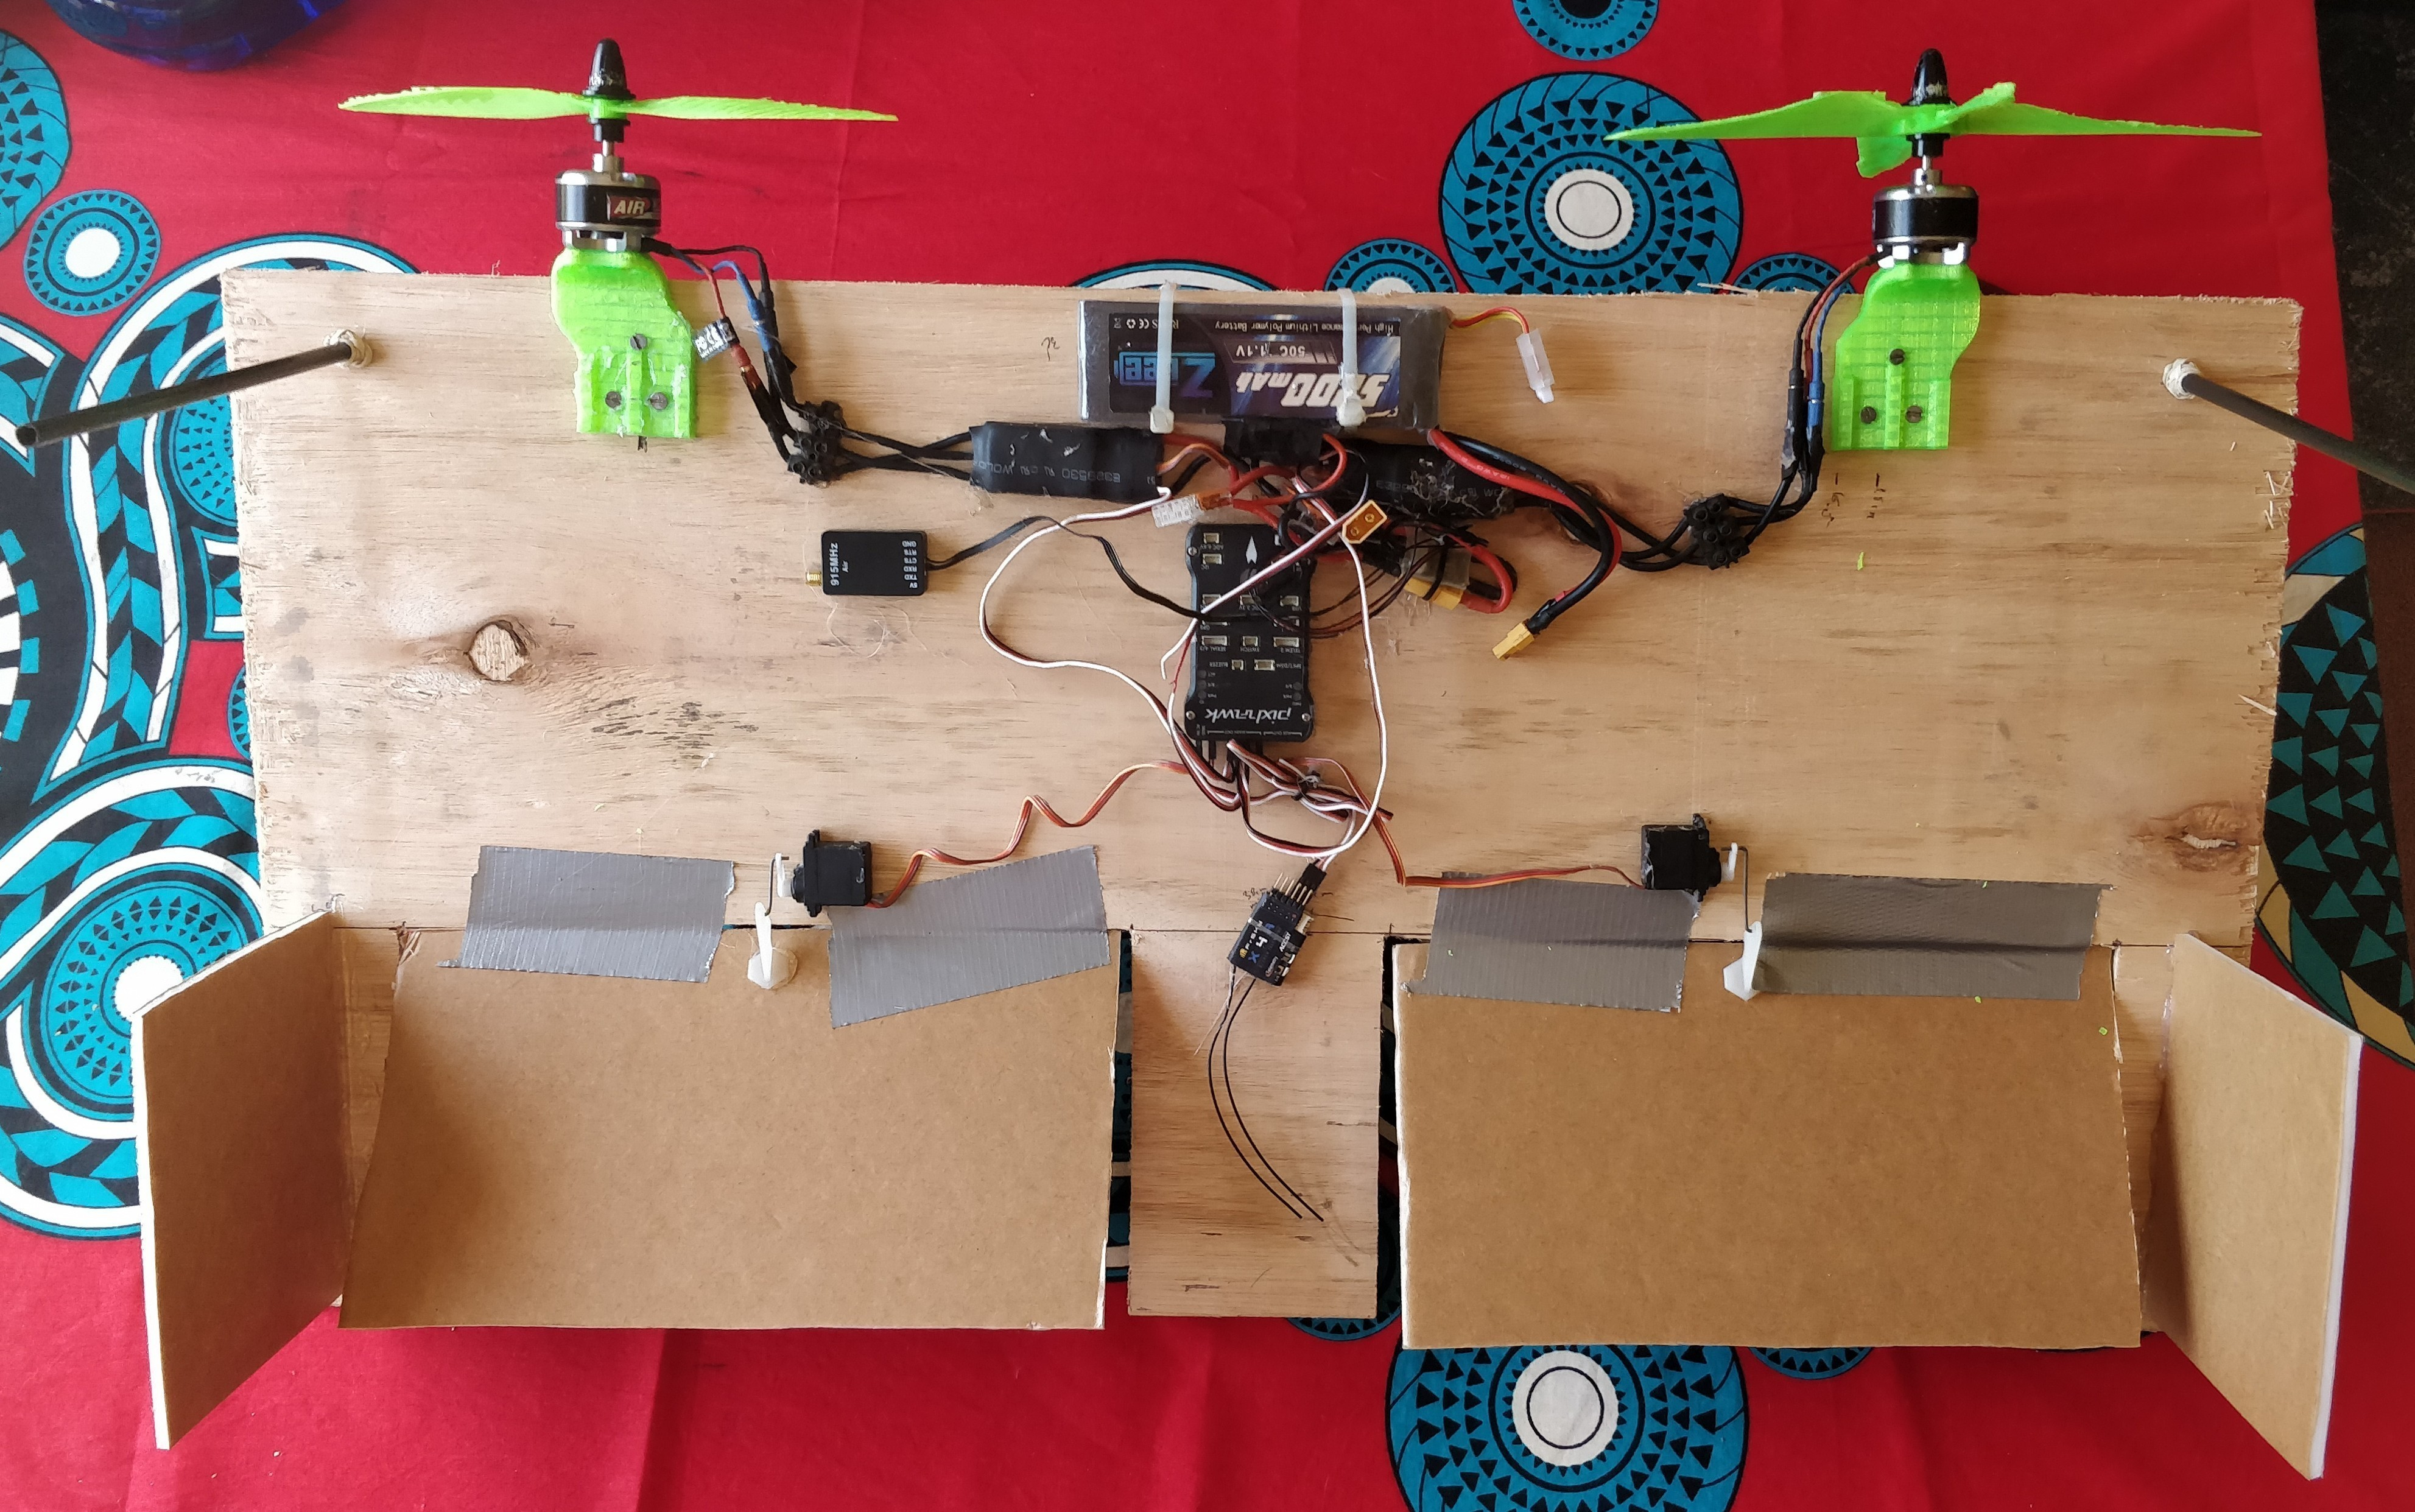
\includegraphics[width=0.7\textwidth]{FlyingBoard.jpg}
    \caption{A picture of the flying board, made out of plywood. The propellers are just placeholders for the photo.}
\end{figure}

After several crashes a few extra modifications were made which can be seen in Figure \ref{fig:finalboard}.
The carbon rods were replaced with vertical pieces of plywood large enough to act as propeller guards but with a small enough area as to not make the aircraft statically unstable in yaw.
The actual area of the front and rear vertical surfaces are equal, but the moment arm to the c.g. is much greater for the rear surfaces making the aircraft still be statically stable in yaw.
After one of the batteries was crushed in a particularly hard crash, turning the battery into ashes, a battery guard was made and mounted.
The engine mounts were slightly reinforced and made straight as well.
The plywood areas under the winglets were broken off in crashes, glued back with carbon rod reinforcements.

\begin{figure}
    \center
    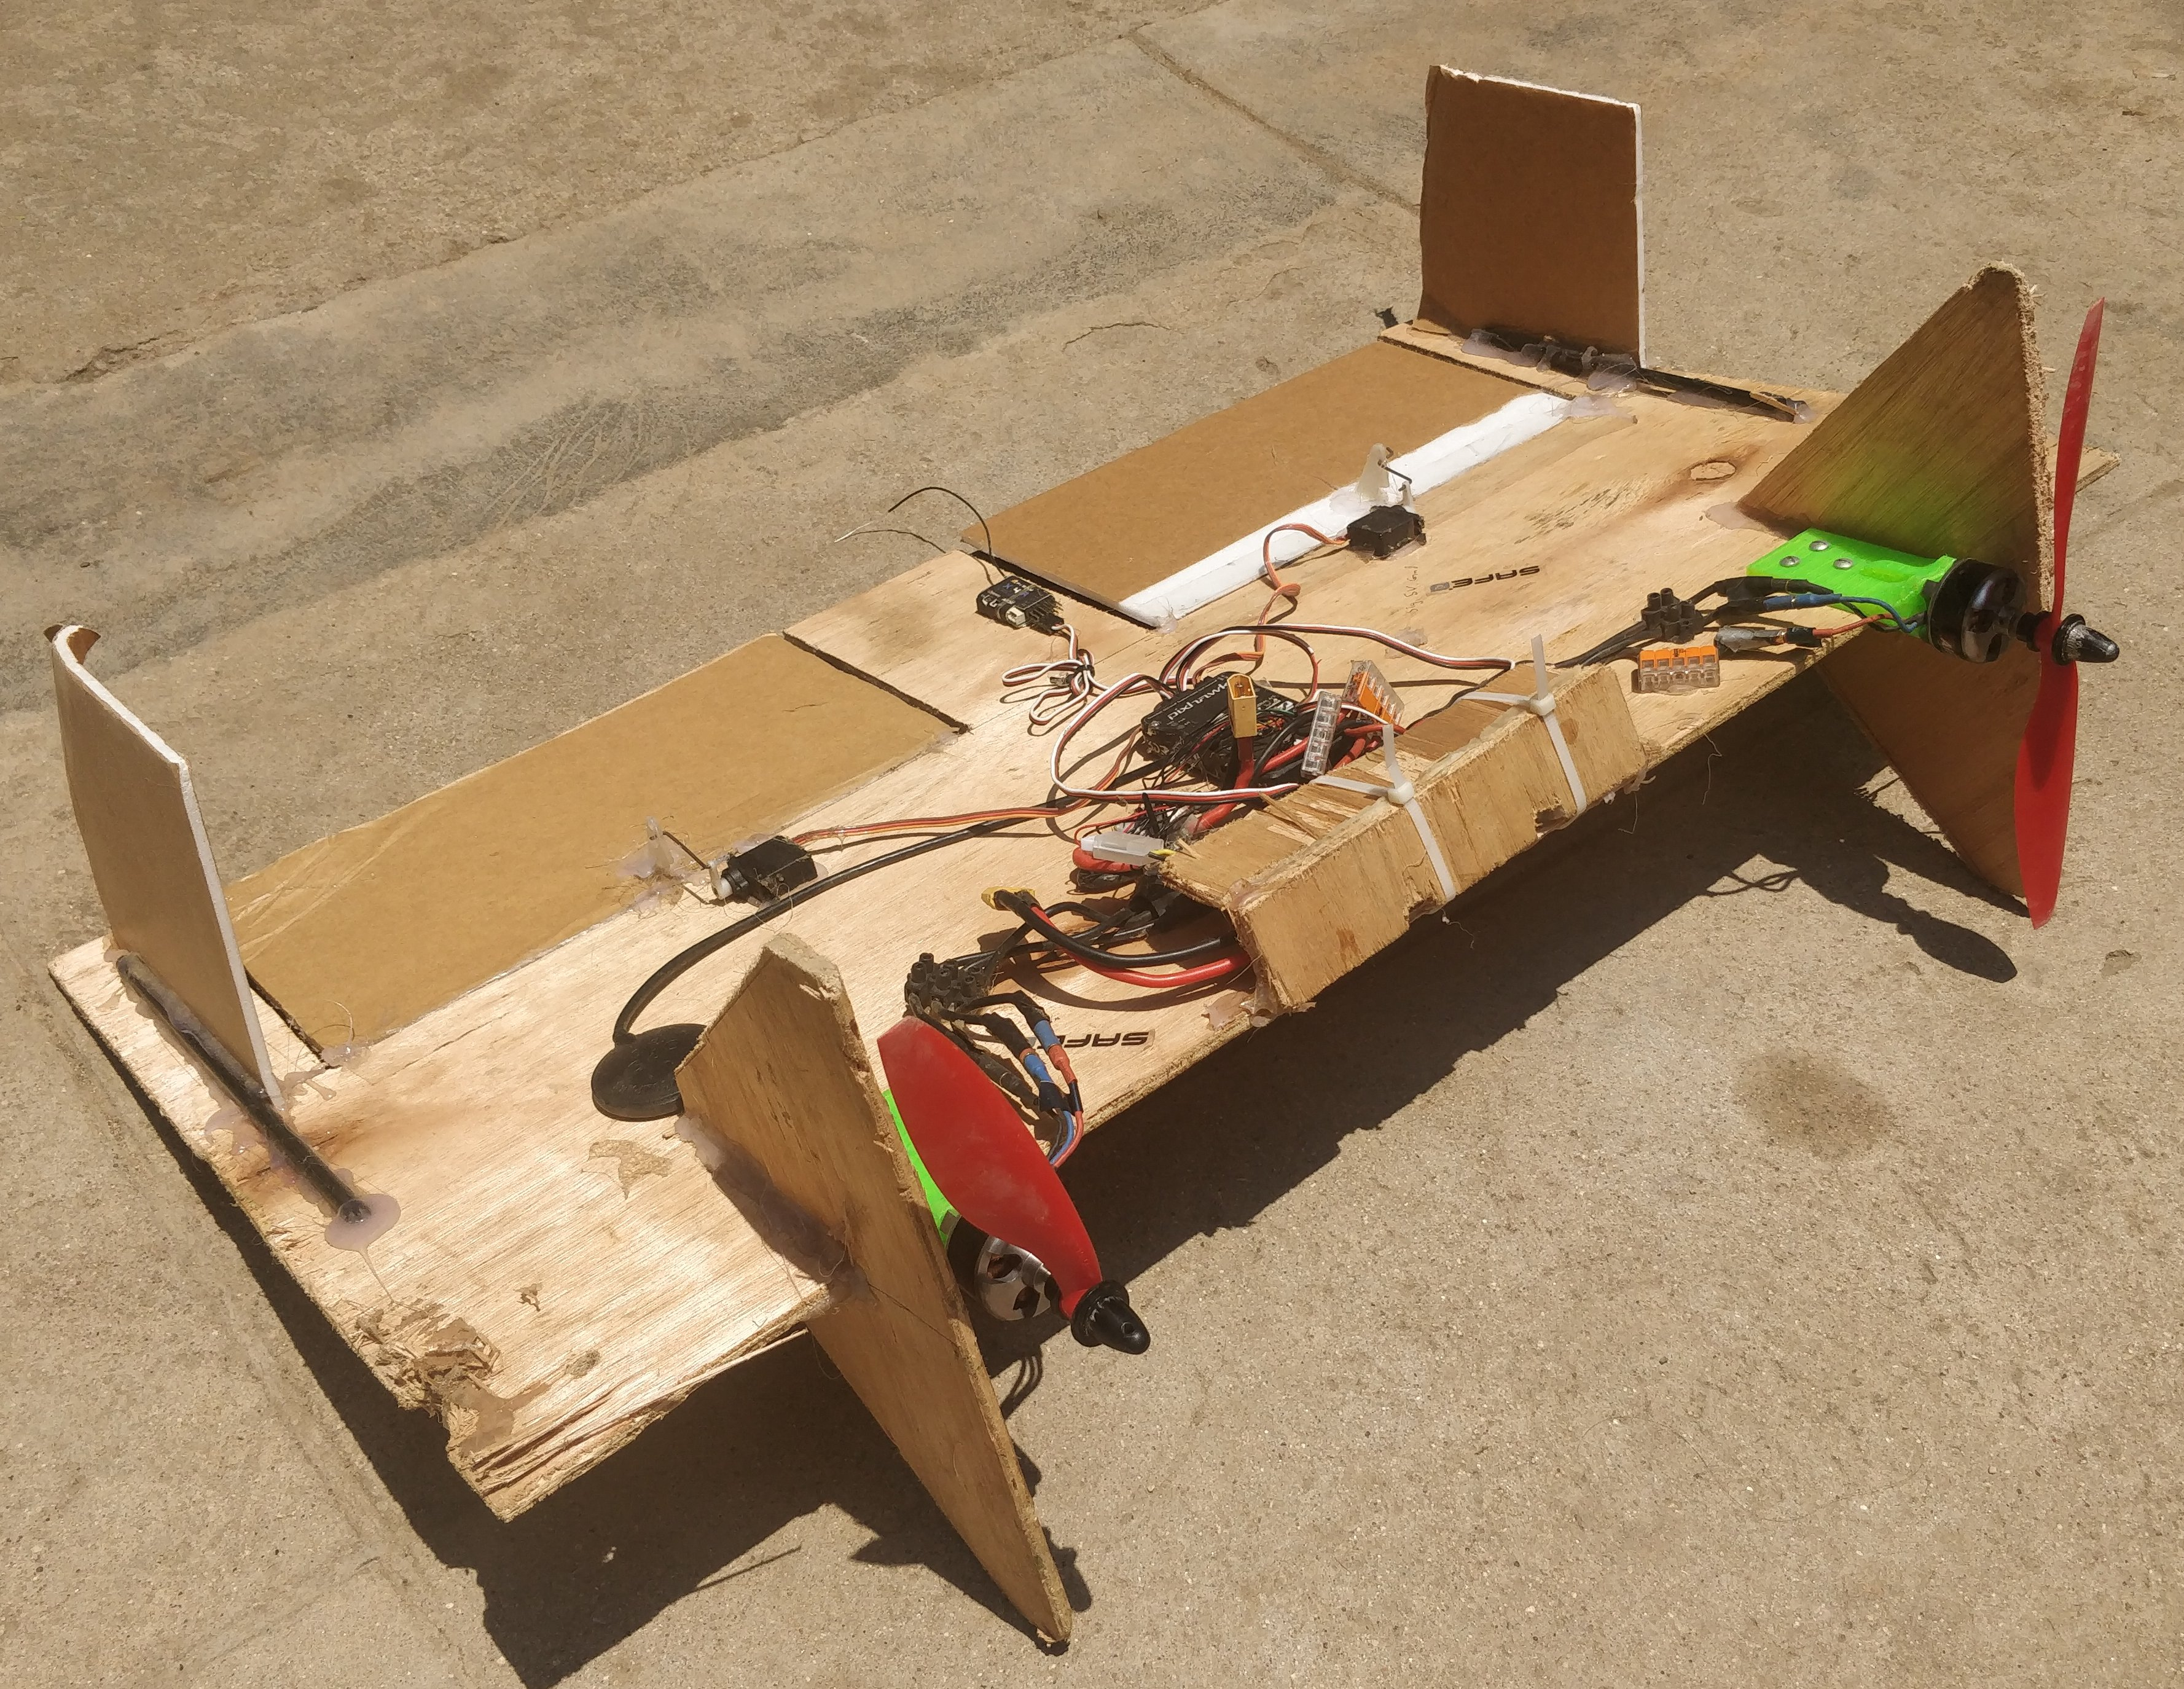
\includegraphics[width=0.7\textwidth]{plywoodfinal.jpg}
    \caption{A picture of the final version of the flying board. The propeller guards have been replaced with plywood, a battery guard has been added, the rear winglet holding areas are reinforced with carbon fibre rods and the gps module is added on the right side.}
    \label{fig:finalboard}
\end{figure}


\subsection{Parameter estimation/declarations}
Most parameters listed can be directly measured on the flying board, such as wing area, weight, center of gravity, etc.
Inertias have been estimated in a CAD program, and other parameters were estimated from measurements/data sheet on similar aircraft.
The simulator is, anyway, just a feasibility check and not a proper tuning ground for the controller, finding bugs and rough settings is good enough.


\section{\textbf{Robust controller development and Implementation}}

The controller implemented is based on a non-linear Proportional squared ($P^2$) controller by Emil Fresk\cite{P2}.
The controller was first implemented on a simulator of the EcoSoar made in Simulink.
A few other controllers were first attempted, among them a Feedback Linearization controller.

\subsection{Feedback Linearization}
Due to the complex nonlinear state space equations solving the system symbolically for feedback simulations was infeasible.
Matlab would compute for days without result and without time estimate.
Filling in certain parameters with numerical values made a semi-symbolic solution possible, which behaved nicely in simulations.
However, the decoupling matrix had a condition number in the order of $10^5$ making the system very susceptible to any noise or uncertainties.
The equations for calculating the necessary actuation also contained very large numbers (order of $10^{80}$) divided by other large numbers meaning that any discrepancies would crash the airplane.

Solving the inverse numerically on the fly was also considered but had similar issues as well as being computationally heavy for a small computer as the Pixhawk 1.
The numerical approach also left no guarantees on existence of solution, because theoretically some of the integrals do have singularities and so the decoupling matrix dependent on them can theoretically be non-invertible in certain (unlikely) situations.

After spending too much time trying to work around these issues the plan was abandoned.


\subsection{Simulink}
The full non linear state space equations derived above in section \ref{sec:fulleqs} were put in a matlab function block surrounded by state integrators to generate the full state.
Parameters were either measured or estimated to complete the numerical simulator.
Controllers could then be tested and evaluated quickly.
An instant 3D render of the simulation was also added through Simulinks VR support blocks.

%TODO: INSERT PICTURE OF SIMULATOR

\subsection{Pixhawk firmware}
Mathworks has support for the embedded coder to directly upload apps into the PX4 NuttX Real Time OS that can run on the Pixhawk 1.
The firmware has to be flashed to PX4 on the Pixhawk, files modified on the SD card and a wide range of supporting softwares must be installed on the host computer.
Mathworks has great documentation on the subject.\cite{MathworksPX4}

\subsection{Initial testing on Bixler}
The evaluate the firmware/simulink controller deployment into a Pixhawk a Bixler was used.
The Pixhawk was put into the Bixler to replace the receiver inside, necessary hardware added and then a simple FlyByWire controller was implemented and uploaded into the Pixhawk from Simulink.
Results were very good, the Bixler flew as expected and no issues with the software on-board.
This was done as a sanity check for the complete software to hardware deployment strategy.


\subsection{P2-controller}
The Pixhawk was then removed from the Bixler and placed on the flying board to test a simple version of the full controller.
The P2 controller \cite{P2} was implemented along with separate tuning for the three axis but a hardcoded, non adjustable, reference attitude of nose up, belly to the north, no logs and no other features.
The controller can be seen in Figure \ref{fig:P2_simulink}

The implemented controller can thus be thought of as a set of three P-D controllers, one for each axis.
The board would hover, but no logs could initially be produced due to a bug in the embedded coder in Simulink.
The sample frequency was set to 120 Hz since the full standard 250 Hz was too much load on the Pixhawk resulting in boot loops after the OS being overrun.
This also allowed the PWM frequency to match the main control loop as anything above 120 Hz was too fast for the servos.

\begin{figure}
    \center
    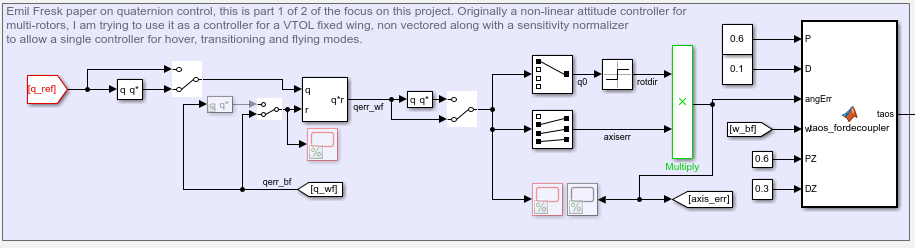
\includegraphics[width=0.9\textwidth]{P2.PNG}
    \caption{The central P2 controller. The manual switches are for debugging, and the very right side block separates the P-D ratios for the propellers (z-axis) from the rest of the system as they require separate tuning.}
    \label{fig:P2_simulink}
\end{figure}

\subsection{Torque translator}
Neither the EcoSoar nor the flying board have propeller wakes that cover the entire elevons.
Therefor it is of interest to normalize the actuation signals to the elevons given the current state so that they produce the requested torque from the P2 controller in any given state.
By assuming that the airflow inside the wake and outside the wake do not affect each other and that the dynamic pressure is the dominating effect a simple function can be found that takes the current rotational speeds of the propellers, the current velocity of the aircraft and requested torque around $x$ and $y$ axis and gives the deflection angle of the control surfaces.

We assume that damping due to rotational speeds do not exist, winglets have no $z$-offset, and no net pitch moment is created by the lift from the wings.
The equations for torque around each axis then become:
\begin{equation}
\begin{split}
    \tau_x =& y_f ( F_L + F_{L_T} - F_{R_T} -F_R) \\
    \tau_y =& x_f ( F_{L_T} + F_L + F_{R_T} + F_R) \\
    \tau_z =& y_T ( T_L - T_R)
\end{split}
\end{equation}
which indicates that the elevons force per deflection is proportional to the airflow speed over them squared.
The P2 controller outputs desired angular acceleration, $\dot{\omega_i}$, not torque.
Necessary torque, $\tau_i$, for axis $i$ is given by
\begin{equation}
    \tau_i = \dot{\omega_i} I_i
\end{equation}
Solving for differential thrust is possible.
Taking the inertia around each axis into account the necessary deflection for each elevon, $u_{\delta_i}$ can be solved for given the current state:
\begin{equation}
\begin{split}
    u_{\delta_L} =& \frac{-0.5 \tau_y}{k_1 sgn(v_x) v^2 + k_2 \omega_L^2} - \frac{0.5 \tau_x}{k_3 sgn(v_x) v^2 + k_4\omega_L^2} \\
    u_{\delta_R} =& \frac{-0.5 \tau_y}{k_1 sgn(v_x) v^2 + k_2 \omega_R^2} + \frac{0.5 \tau_x}{k_3 sgn(vx) v^2 + k_4 \omega_R^2} 
\end{split}
\label{eq:TT}
\end{equation}
where $k_{[1-4]}$ are numerical constants given by aircraft parameters.

The torque translator is implemented in the Simulink controller as a matlab function, which can be seen in Figure \ref{fig:TT}.
\begin{figure}
    \center
    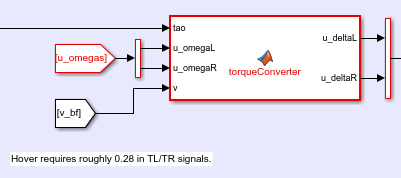
\includegraphics[width=0.6\textwidth]{TT.PNG}
    \caption{Controller implementation of equation \ref{eq:TT}.}
    \label{fig:TT}
\end{figure}

\subsubsection{Finding $k_2$ and $k_4$}
Bypassing the torque translator and running the controller directly to the control surfaces a suitable step response can be tuned in while hovering.
While hovering still in the air $v_x$ can be assumed to be negligible, and thus once the wanted response has been found one can solve for $k_2$ and $k_4$; the rotational speeds are known signals.

\subsubsection{Finding $k_1$ and $k_3$: Single Engine Board}
By flying normally with a standard Fly By Wire system and PD controller for pitch and roll a suitable response can be tuned in, granted that the board only has one single engine which propeller wash does not interfere with the control surfaces.
This means that one can assume the contribution from the terms $k_2$ and $k_4$ are included in to be zero.
Since velocity and the ratio torque/actuation is known the remaining parameters can be found.

For this very task an 80\% scale model of the flying plywood board was built, but with a single engine in the front instead of two.

\begin{figure}
    \center
    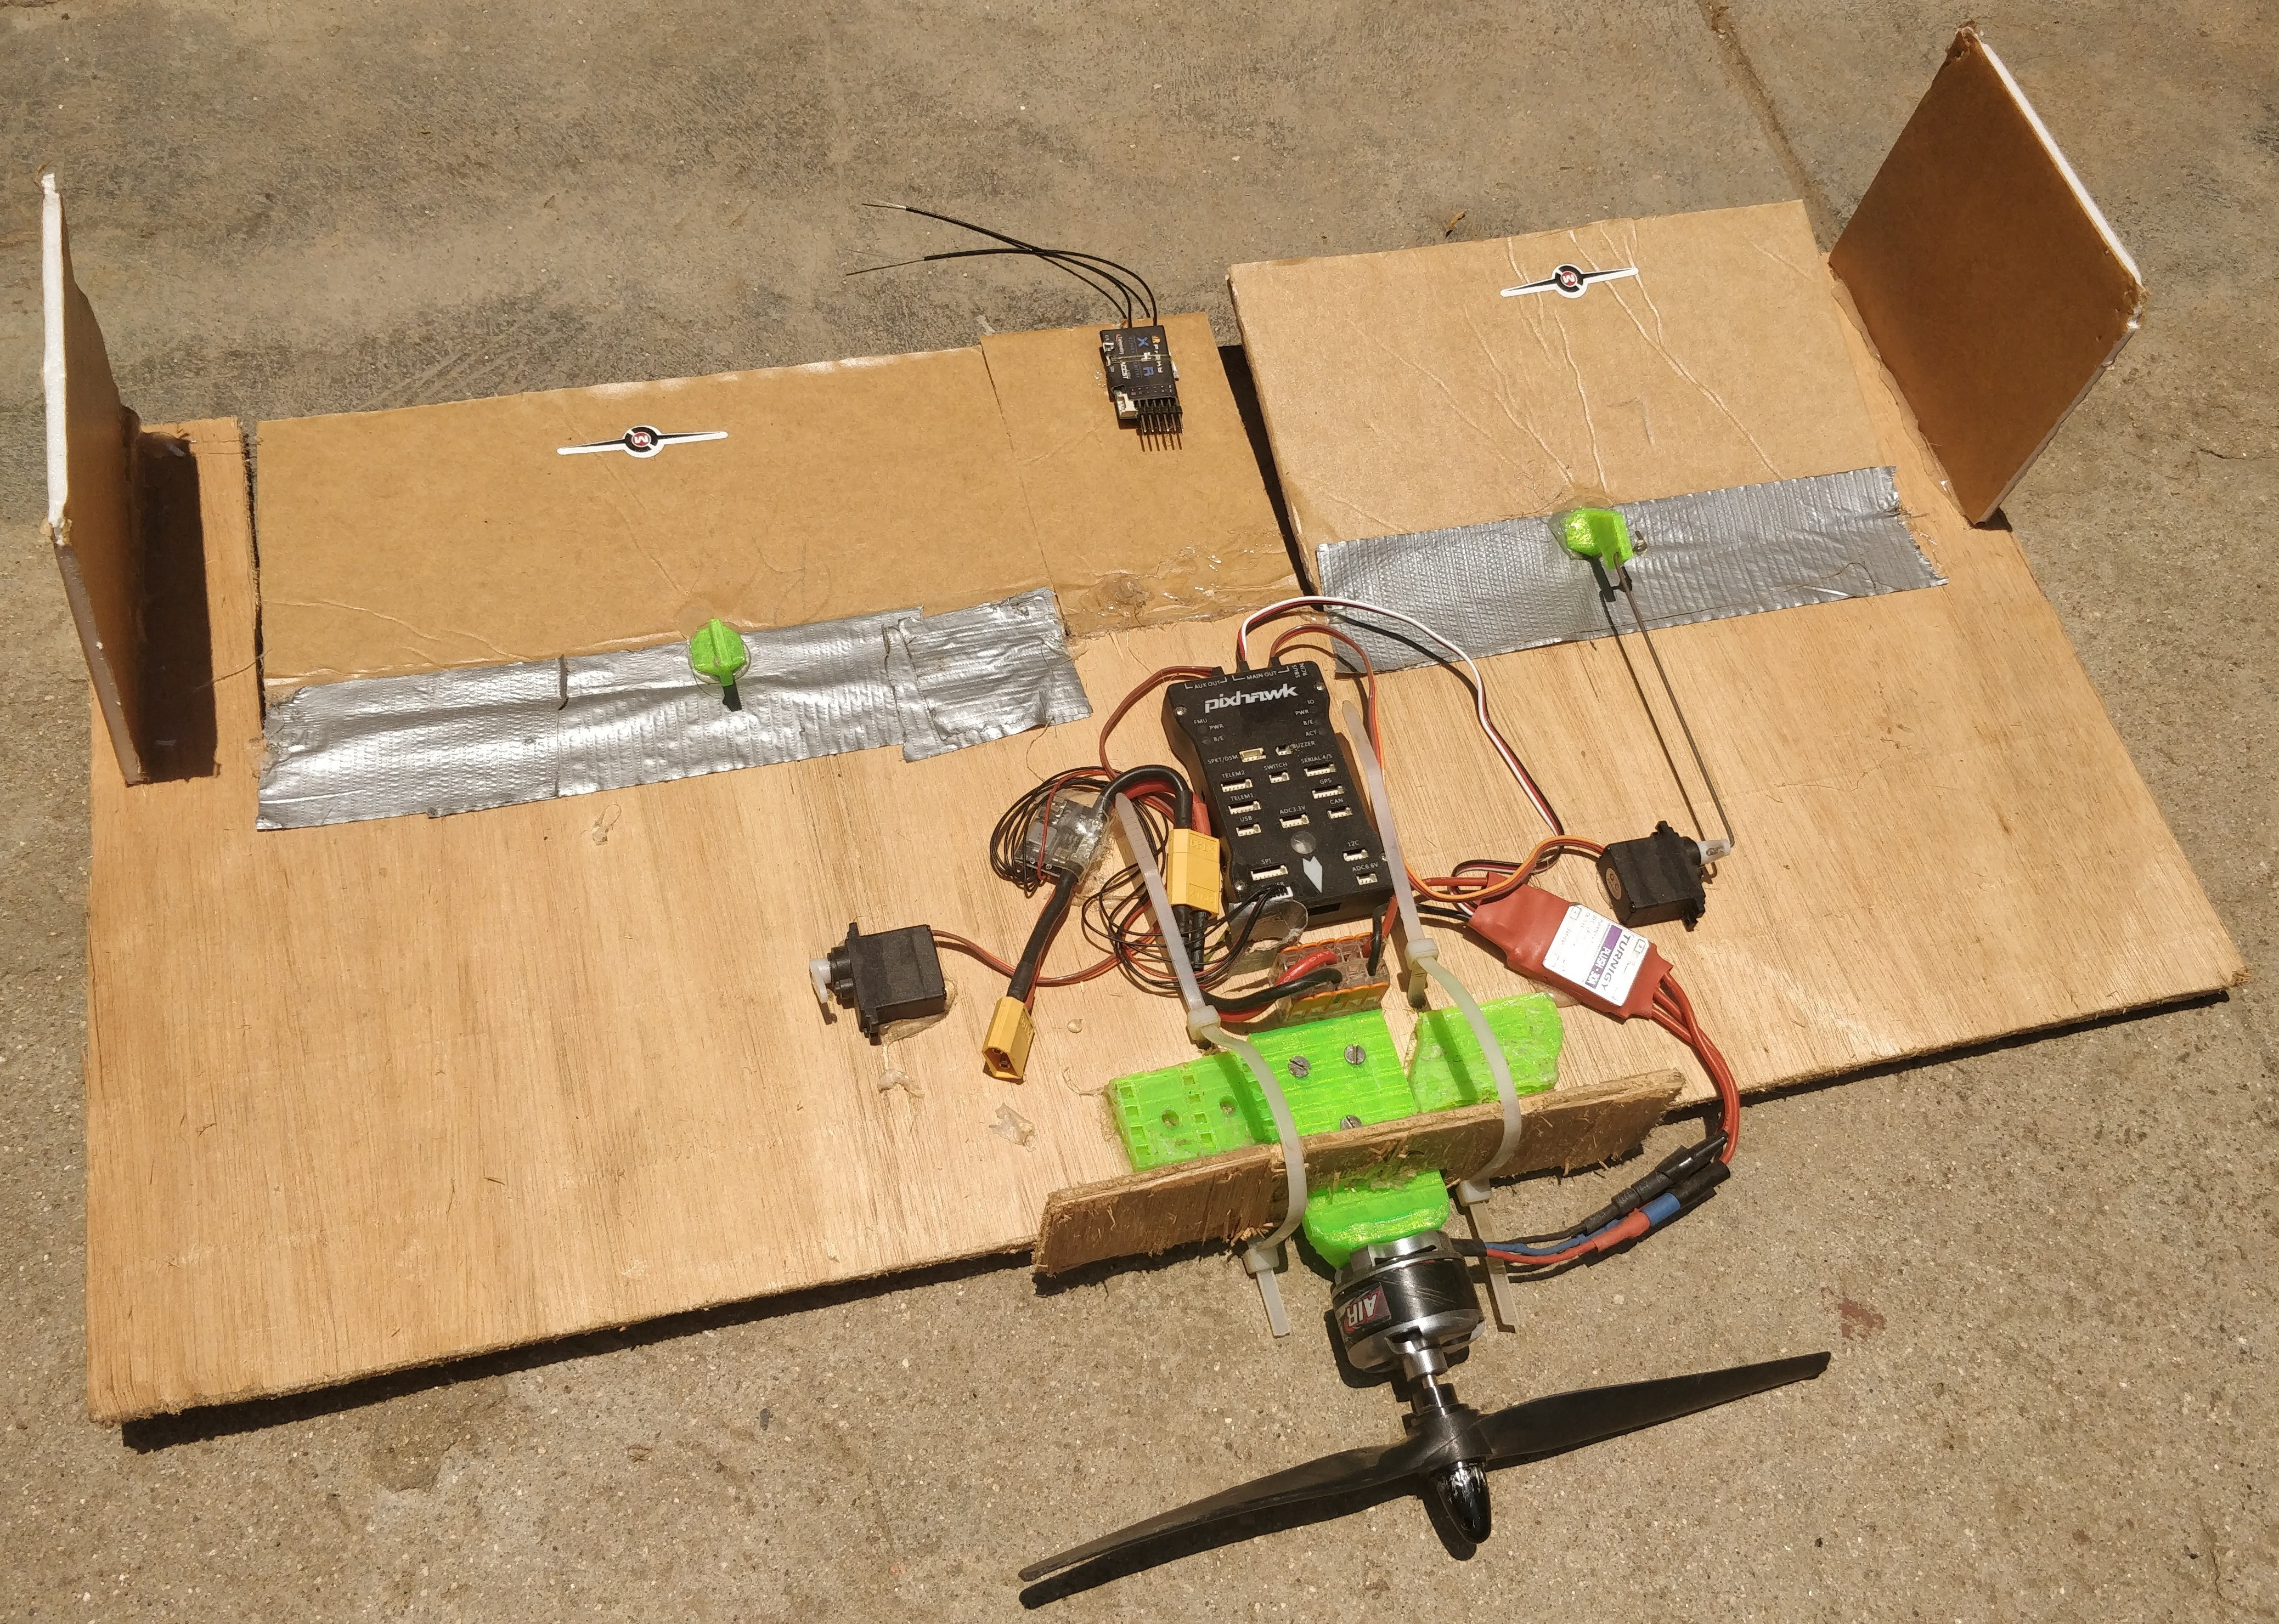
\includegraphics[width=0.7\textwidth]{singleengine.jpg}
    \caption{A picture of the 80\% scale model, single engine version, flying board used for parameter estimation.}
    \label{fig:singleengine}
\end{figure}

This test only gives a rough estimate, however, since the propeller wash does cover the elevons partially.
A rear mounted propeller would have been better but there was no way to keep the c.g. in front of the center of pressure without a complete redesign of the aircraft had the engine been mounted in the rear.
Therefore the parameter estimations found through flying this board only serve to find rough estimates good enough for flying the dual engine one without crashing instantly.

\subsection{Full controller diagram}
The full controller has an adjustable reference quaternion generated by user inputs on the transmitter, a manual emergency motor and servo shutdown, an altitude holder, SD signal logging blocks, a step response generator, low battery voltage protection cutoff and LED control for the onboard led to indicate arming state and GPS accuracy.

The horizontal layout of the Simulink blocks in the full controller make an overview picture difficult.
The full schematics can instead be found in the git repo.\cite{mycode}

In Figure \ref{fig:q_wf} the quaternion and angular rates from the Extended Kalman Filter for attitude estimation in the firmware is read.
In Figure \ref{fig:qref} the reference quaternion is generated.
The reference quaternion, estimated quaternion and angular rates are passed onto the P2 controller shown in Figure \ref{fig:P2_simulink}.
The reference quaternion can be modified by the step function generator shown in Figure \ref{fig:step}.
The emergency shutoff function is shown in Figure \ref{fig:stop}.

The battery voltage reading is low pass filtered due to large noise in the signal trigging short engine cutouts in flight.
The lowest allowed cell voltage is on purpose set quite low due to voltage being much lower under load.
A 3 Volt per cell cutoff results in the resting voltage stabilizing around 3.5 without load which is more than a safe discharge voltage.

\begin{figure}
    \center
    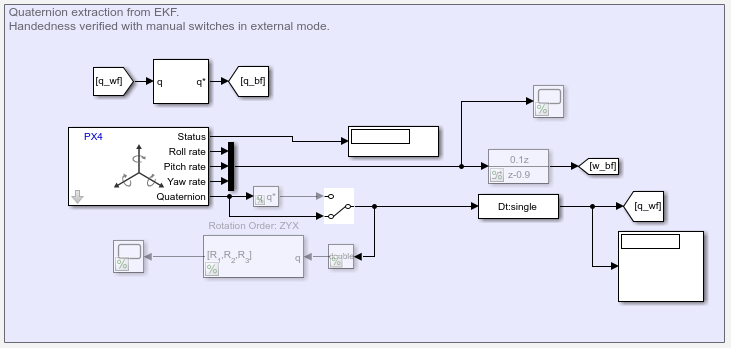
\includegraphics[width=0.7\textwidth]{q_wf.PNG}
    \caption{The quaternion estimation retrieval from the Pixhawk firmware.}
    \label{fig:q_wf}
\end{figure}
\begin{figure}
    \center
    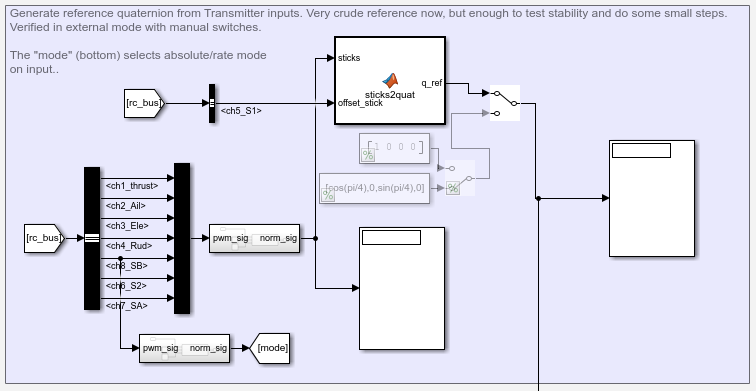
\includegraphics[width=0.7\textwidth]{qref.PNG}
    \caption{The quaternion reference generation, modified with RC inputs.}
    \label{fig:qref}
\end{figure}
\begin{figure}
    \center
    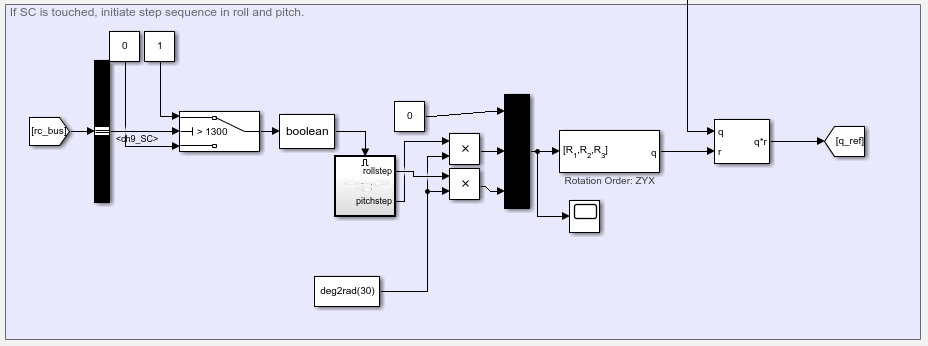
\includegraphics[width=0.7\textwidth]{step.PNG}
    \caption{The attitude step generation routine.}
    \label{fig:step}
\end{figure}
\begin{figure}
    \center
    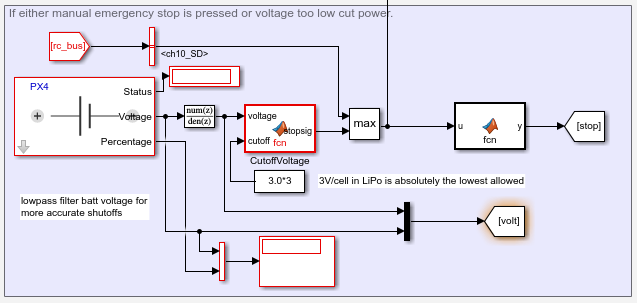
\includegraphics[width=0.7\textwidth]{stop.PNG}
    \caption{Emergency shutoff routine which overrides all outputs should it be necessary.}
    \label{fig:stop}
\end{figure}

\section{Results}

The plywood board can hover and transition into flight.
Further tuning would be preferable but not possible for the scope of this thesis due to time and weather constraints.

\subsection{Performance in Simulations}
Since all parameters are well known/set in the simulator and assumptions are the same for the simulator and controller the system works very well in simulation for a very wide range of parameters and settings.
Therefore it does not yield any valuable tuning reference frame, only general info like testing handedness of quaternions and whether the controller is at all feasible.


%TODO: Maybe add graphs of simulations?
%The simulations worked so well with almost any settings maybe they aren't of interest?

\subsection{Performance of the flying plywood board in reality}
The board hovers and flies controllably.
To achieve very smooth flight more tuning is necessary but the fact that it flies at all without the need of any switching controller indicates that the concept of normalizing the sensitivity of the control surfaces is very much valid.

In Figure \ref{fig:pitchstep} and \ref{fig:rollstep} step responses in pitch and roll while both hovering and flying are displayed.
The responses are similar but of different gain.
A small oscillation can be seen in the response while flying.

In Figure \ref{fig:transition} a complete transition from hovering to flying can be seen.
The reference pitch had to be manually adjusted during the transition to maintain level flight; no altitude holder was enabled.


\begin{figure}[]
    \centering
    % This file was created by matlab2tikz.
%
%The latest updates can be retrieved from
%  http://www.mathworks.com/matlabcentral/fileexchange/22022-matlab2tikz-matlab2tikz
%where you can also make suggestions and rate matlab2tikz.
%
\definecolor{mycolor1}{rgb}{0.00000,0.44700,0.74100}%
\definecolor{mycolor2}{rgb}{0.85000,0.32500,0.09800}%
\definecolor{mycolor3}{rgb}{0.92900,0.69400,0.12500}%
\definecolor{mycolor4}{rgb}{0.49400,0.18400,0.55600}%
%
\begin{tikzpicture}

\begin{axis}[%
width=4.521in,
height=3.566in,
at={(0.758in,0.481in)},
scale only axis,
xmin=0,
xmax=4.5,
xlabel style={font=\color{white!15!black}},
xlabel={Time [seconds]},
ymin=-0.5,
ymax=2,
ylabel style={font=\color{white!15!black}},
ylabel={Pitch angle [radians]},
axis background/.style={fill=white},
title style={font=\bfseries},
title={Pitch step responses},
axis x line*=bottom,
axis y line*=left,
legend style={at={(0.061,0.5)}, anchor=south west, legend cell align=left, align=left, draw=white!15!black}
]
\addplot [color=mycolor1]
  table[row sep=crcr]{%
0	0.140780909412358\\
0.0249810000000252	0.138718230186651\\
0.04988400000002	0.135078914897544\\
0.0749700000000075	0.134854695695169\\
0.0999229999999898	0.136303792795106\\
0.125395000000026	0.1316930109644\\
0.15032599999995	0.122550955816316\\
0.174939999999992	0.117073473253825\\
0.200317000000041	0.121307843724882\\
0.224945999999932	0.130299023593064\\
0.249856000000023	0.136746137664161\\
0.274915999999962	0.137337441345697\\
0.300297	0.132194935392657\\
0.324986999999965	0.126574149583585\\
0.349846999999954	0.126560031909042\\
0.37491	0.131809738483742\\
0.399847000000022	0.143088204598196\\
0.424945999999977	0.148843396840192\\
0.449906999999939	0.14793448374274\\
0.475340999999958	0.149105318257637\\
0.500014999999962	0.168746528819951\\
0.524976000000038	0.202228439184795\\
0.549892	0.240571850543293\\
0.574979999999982	0.269418729878879\\
0.599884999999972	0.280024292770741\\
0.624991000000023	0.274816377635442\\
0.649856	0.263933048648231\\
0.674913999999944	0.266270277075818\\
0.700015000000008	0.281613912478756\\
0.725076999999942	0.302339275693509\\
0.74985700000002	0.320058905317497\\
0.77491299999997	0.325028882362837\\
0.799913999999944	0.324537742408307\\
0.824990999999955	0.327359944953224\\
0.849886999999967	0.338722248075608\\
0.874903000000018	0.350977052536168\\
0.899847000000022	0.359870508028038\\
0.924999999999955	0.361788848497223\\
0.949847999999974	0.3622596008872\\
0.974947000000043	0.366399516287391\\
0.999841999999944	0.375562771985802\\
1.02495299999998	0.387531032726729\\
1.04983900000002	0.399456574544927\\
1.074926	0.405657032809125\\
1.09998699999994	0.409437818107064\\
1.12505099999998	0.413972930215791\\
1.14988500000004	0.420041857017113\\
1.17492200000004	0.425233846075118\\
1.19993899999997	0.430594771971921\\
1.22503099999994	0.433807529298253\\
1.24991399999999	0.431757625165226\\
1.27493500000003	0.427078434629177\\
1.29985699999997	0.425710474782221\\
1.32505800000001	0.431070711540735\\
1.34987699999999	0.444448459775137\\
1.37501399999996	0.45520137537472\\
1.39983099999995	0.459556516191374\\
1.42498399999999	0.458441245328394\\
1.45436199999995	0.449976632213652\\
1.47628699999996	0.437502166363461\\
1.49984299999994	0.416837097191207\\
1.52489700000001	0.395622069097642\\
1.54979800000001	0.378100483619127\\
1.57495299999994	0.365647623525884\\
1.60030399999994	0.358103072701834\\
1.62493699999993	0.350301309711033\\
1.64980000000003	0.341846944753183\\
1.67555100000004	0.332193119137349\\
1.699792	0.32491105526871\\
1.72489199999995	0.318804348267218\\
1.74982799999998	0.314233548585236\\
1.77481399999999	0.308893860689982\\
1.79992000000004	0.303863353799627\\
1.84982000000002	0.295731545768438\\
1.87544800000001	0.291481962937261\\
1.89985899999999	0.287807578791449\\
1.92493100000002	0.284641402564349\\
1.94982600000003	0.28146356241295\\
1.97495500000002	0.278198851946039\\
1.99983099999997	0.274938989248128\\
2.02503300000001	0.270483691313266\\
2.04978500000004	0.267006505292567\\
2.07519600000001	0.265120303697728\\
2.10002999999995	0.26489451219477\\
2.12490400000002	0.264818113791402\\
2.14981899999998	0.263457088815185\\
2.17490299999997	0.260316918357463\\
2.19977299999994	0.257691124279717\\
2.22489999999993	0.25492196490766\\
2.24977000000001	0.252609264319891\\
2.27533299999993	0.250186716963444\\
2.30006200000003	0.247598117115308\\
2.32489599999997	0.24455820729476\\
2.34977000000003	0.241654314651127\\
2.37491899999998	0.240888005414849\\
2.39977799999997	0.242288877774746\\
2.42492600000003	0.243488053103453\\
2.44981699999994	0.243125670327952\\
2.47477900000001	0.236160637020222\\
2.5	0.211357074213395\\
2.524946	0.177751093487231\\
2.54985999999997	0.141847759543428\\
2.57488599999999	0.112140737894077\\
2.60135200000002	0.086968073945054\\
2.62636099999997	0.0699651332165546\\
2.65031699999997	0.0562791407434221\\
2.67496500000004	0.0434494696590094\\
2.70013299999994	0.0278973281400877\\
2.72497399999997	0.0142519963053864\\
2.74977200000001	0.0017005233199066\\
2.77476899999999	-0.00870769115704377\\
2.80027799999993	-0.019637714309179\\
2.82495199999994	-0.0294136756867412\\
2.85034899999994	-0.0388060458701181\\
2.87492099999997	-0.0468634126157867\\
2.90013999999996	-0.0563996984338132\\
2.92491799999993	-0.0639891499584107\\
2.94975799999997	-0.0707085250779748\\
2.97476299999994	-0.0763007092109654\\
3.00133900000003	-0.0832076098126807\\
3.02488400000004	-0.0917668588377829\\
3.04977299999996	-0.102403284451049\\
3.07478300000002	-0.113847054024759\\
3.10010899999997	-0.125959451979487\\
3.12487899999996	-0.134139086146547\\
3.15041299999996	-0.139806947332827\\
3.17479600000001	-0.143430511037304\\
3.199838	-0.146096642348968\\
3.22491600000001	-0.149000579479948\\
3.24977999999999	-0.153430553719462\\
3.27617299999997	-0.160536549181947\\
3.29996500000004	-0.166214496645692\\
3.324928	-0.169444240576369\\
3.34978699999999	-0.170055468517598\\
3.374773	-0.1701675697441\\
3.39974199999995	-0.17058456314263\\
3.42502100000002	-0.172164682177807\\
3.44985999999994	-0.175551350260513\\
3.47472600000003	-0.180670701667678\\
3.50013999999999	-0.176494276598523\\
3.52478199999996	-0.155069768046408\\
3.54971899999998	-0.122433481493567\\
3.57476499999996	-0.0881508764703409\\
3.59971699999994	-0.0621884114980523\\
3.62508100000002	-0.0566378303931226\\
3.64971500000001	-0.0583142275309894\\
3.674712	-0.0581189556006633\\
3.70021799999995	-0.0493846044526811\\
3.72489599999994	-0.0369298610070678\\
3.750362	-0.0221301649244138\\
3.77470800000003	-0.0162141615043444\\
3.79970900000001	-0.0128871388122265\\
3.82492300000001	-0.00775050021301329\\
3.84977500000002	-0.00239402927946466\\
3.87475199999994	-0.000688275798168788\\
3.89972	0.00224526360739819\\
3.92488600000001	0.00907647019779877\\
3.94978400000002	0.0157110905704552\\
3.97475999999995	0.0145558787411063\\
3.999731	0.0103710394205918\\
4.02480200000002	0.0121497966427996\\
4.04975400000001	0.0228162414120181\\
4.07469600000002	0.0307640408878784\\
4.09973100000002	0.0323680613104453\\
4.12490100000002	0.0306116330606321\\
4.14970800000003	0.0293197668395224\\
4.17469600000004	0.0301737908111573\\
4.20026999999993	0.0345822061452876\\
4.22496999999998	0.0409661840370291\\
4.24974699999996	0.0490106140827656\\
4.27468999999996	0.0554621906042462\\
4.29968699999995	0.0604343122164841\\
4.32476199999996	0.063714809441619\\
4.34968600000002	0.067659016396679\\
4.37476400000003	0.0731321298852844\\
4.39997800000003	0.0801092066256086\\
4.42476399999998	0.0851514644155317\\
4.44968600000004	0.0866510409545738\\
4.47534599999994	0.0860369318601827\\
};
\addlegendentry{flying}

\addplot [color=mycolor2]
  table[row sep=crcr]{%
0	0.178259613561653\\
0.0249810000000252	0.178259613561653\\
0.04988400000002	0.178259613561653\\
0.0749700000000075	0.178259613561653\\
0.0999229999999898	0.178259613561653\\
0.125395000000026	0.178259613561653\\
0.15032599999995	0.178259613561653\\
0.174939999999992	0.178259613561653\\
0.200317000000041	0.178259613561653\\
0.224945999999932	0.178259613561653\\
0.249856000000023	0.178259613561653\\
0.274915999999962	0.178259613561653\\
0.300297	0.178259613561653\\
0.324986999999965	0.178259613561653\\
0.349846999999954	0.178266273272203\\
0.37491	0.178259613561653\\
0.399847000000022	0.178266273272203\\
0.424945999999977	0.679816695131013\\
0.449906999999939	0.679538691989525\\
0.475340999999958	0.679538691989525\\
0.500014999999962	0.679816695131013\\
0.524976000000038	0.679816695131013\\
0.549892	0.679816695131013\\
0.574979999999982	0.679816695131013\\
0.599884999999972	0.679816695131013\\
0.624991000000023	0.679816695131013\\
0.649856	0.679816695131013\\
0.674913999999944	0.679816695131013\\
0.700015000000008	0.679816695131013\\
0.725076999999942	0.679816695131013\\
0.74985700000002	0.679816695131013\\
0.77491299999997	0.679816695131013\\
0.799913999999944	0.679816695131013\\
0.824990999999955	0.679816695131013\\
0.849886999999967	0.679816695131013\\
0.874903000000018	0.679816695131013\\
0.899847000000022	0.679816695131013\\
0.924999999999955	0.679816695131013\\
0.949847999999974	0.679816695131013\\
0.974947000000043	0.679816695131013\\
0.999841999999944	0.679816695131013\\
1.02495299999998	0.679816695131013\\
1.04983900000002	0.679816695131013\\
1.074926	0.679816695131013\\
1.09998699999994	0.679816695131013\\
1.12505099999998	0.679816695131013\\
1.14988500000004	0.679816695131013\\
1.17492200000004	0.679816695131013\\
1.19993899999997	0.679816695131013\\
1.22503099999994	0.679816695131013\\
1.24991399999999	0.679816695131013\\
1.27493500000003	0.679816695131013\\
1.29985699999997	0.679816695131013\\
1.32505800000001	0.679816695131013\\
1.34987699999999	0.679816695131013\\
1.37501399999996	0.679538691989525\\
1.39983099999995	0.679816695131013\\
1.42498399999999	0.178259613561653\\
1.45436199999995	0.178266273272203\\
1.47628699999996	0.178266273272203\\
1.49984299999994	0.178259613561653\\
1.52489700000001	0.178266273272203\\
1.54979800000001	0.178266273272203\\
1.57495299999994	0.178266273272203\\
1.60030399999994	0.178266273272203\\
1.62493699999993	0.178266273272203\\
1.64980000000003	0.178266273272203\\
1.67555100000004	0.178266273272203\\
1.699792	0.178266273272203\\
1.72489199999995	0.178266273272203\\
1.74982799999998	0.178266273272203\\
1.77481399999999	0.178266273272203\\
1.79992000000004	0.178266273272203\\
1.84982000000002	0.178266273272203\\
1.87544800000001	0.178266273272203\\
1.89985899999999	0.178259613561653\\
1.92493100000002	0.178259613561653\\
1.94982600000003	0.178266273272203\\
1.97495500000002	0.178266273272203\\
1.99983099999997	0.178259613561653\\
2.02503300000001	0.178266273272203\\
2.04978500000004	0.178259613561653\\
2.07519600000001	0.178259613561653\\
2.10002999999995	0.178266273272203\\
2.12490400000002	0.178266273272203\\
2.14981899999998	0.178259613561653\\
2.17490299999997	0.178266273272203\\
2.19977299999994	0.178266273272203\\
2.22489999999993	0.178266273272203\\
2.24977000000001	0.178266273272203\\
2.27533299999993	0.178266273272203\\
2.30006200000003	0.178259613561653\\
2.32489599999997	0.178259613561653\\
2.34977000000003	0.178259613561653\\
2.37491899999998	0.178266273272203\\
2.39977799999997	0.178266273272203\\
2.42492600000003	0.178259613561653\\
2.44981699999994	-0.313500375172131\\
2.47477900000001	-0.313843561670783\\
2.5	-0.313500375172131\\
2.524946	-0.313500375172131\\
2.54985999999997	-0.313500375172131\\
2.57488599999999	-0.313843561670783\\
2.60135200000002	-0.313500375172131\\
2.62636099999997	-0.313500375172131\\
2.65031699999997	-0.313500375172131\\
2.67496500000004	-0.313500375172131\\
2.70013299999994	-0.313500375172131\\
2.72497399999997	-0.313500375172131\\
2.74977200000001	-0.313500375172131\\
2.77476899999999	-0.313843561670783\\
2.80027799999993	-0.313500375172131\\
2.82495199999994	-0.313843561670783\\
2.85034899999994	-0.313843561670783\\
2.87492099999997	-0.313843561670783\\
2.90013999999996	-0.313843561670783\\
2.92491799999993	-0.313843561670783\\
2.94975799999997	-0.313843561670783\\
2.97476299999994	-0.313500375172131\\
3.00133900000003	-0.313500375172131\\
3.02488400000004	-0.313500375172131\\
3.04977299999996	-0.313843561670783\\
3.07478300000002	-0.313843561670783\\
3.10010899999997	-0.313843561670783\\
3.12487899999996	-0.313843561670783\\
3.15041299999996	-0.313843561670783\\
3.17479600000001	-0.313843561670783\\
3.199838	-0.313843561670783\\
3.22491600000001	-0.313843561670783\\
3.24977999999999	-0.313500375172131\\
3.27617299999997	-0.313500375172131\\
3.29996500000004	-0.313500375172131\\
3.324928	-0.313843561670783\\
3.34978699999999	-0.313843561670783\\
3.374773	-0.313843561670783\\
3.39974199999995	-0.313843561670783\\
3.42502100000002	-0.313500375172131\\
3.44985999999994	0.178266273272203\\
3.47472600000003	0.178266273272203\\
3.50013999999999	0.178266273272203\\
3.52478199999996	0.178266273272203\\
3.54971899999998	0.178266273272203\\
3.57476499999996	0.178266273272203\\
3.59971699999994	0.178266273272203\\
3.62508100000002	0.178266273272203\\
3.64971500000001	0.178266273272203\\
3.674712	0.178266273272203\\
3.70021799999995	0.178266273272203\\
3.72489599999994	0.178266273272203\\
3.750362	0.178259613561653\\
3.77470800000003	0.178259613561653\\
3.79970900000001	0.178266273272203\\
3.82492300000001	0.178266273272203\\
3.84977500000002	0.178266273272203\\
3.87475199999994	0.178266273272203\\
3.89972	0.178266273272203\\
3.92488600000001	0.178266273272203\\
3.94978400000002	0.178266273272203\\
3.97475999999995	0.178259613561653\\
3.999731	0.178259613561653\\
4.02480200000002	0.178266273272203\\
4.04975400000001	0.178266273272203\\
4.07469600000002	0.178266273272203\\
4.09973100000002	0.178266273272203\\
4.12490100000002	0.178266273272203\\
4.14970800000003	0.178266273272203\\
4.17469600000004	0.178266273272203\\
4.20026999999993	0.178259613561653\\
4.22496999999998	0.178259613561653\\
4.24974699999996	0.178259613561653\\
4.27468999999996	0.178259613561653\\
4.29968699999995	0.178259613561653\\
4.32476199999996	0.178956426698487\\
4.34968600000002	0.178259613561653\\
4.37476400000003	0.178259613561653\\
4.39997800000003	0.178266273272203\\
4.42476399999998	0.178266273272203\\
4.44968600000004	0.178259613561653\\
4.47534599999994	0.178259613561653\\
};
\addlegendentry{flying reference}

\addplot [color=mycolor3]
  table[row sep=crcr]{%
0	1.29831866225429\\
0.0250520000000733	1.29995842161957\\
0.0501649999999927	1.30081279879535\\
0.074971000000005	1.30175378125223\\
0.0999820000000682	1.30321793802566\\
0.124969000000078	1.30554474032972\\
0.15003999999999	1.30801281671696\\
0.175009000000045	1.31021009699823\\
0.199962000000028	1.31277705204679\\
0.224961000000008	1.31579943461807\\
0.250036000000023	1.31713307402785\\
0.274959000000081	1.31823840093028\\
0.300004000000058	1.31956591293953\\
0.32496100000003	1.32105586927614\\
0.35003800000004	1.32184729666986\\
0.374962000000096	1.32319208949067\\
0.400074000000018	1.32440642205713\\
0.424982999999997	1.32547807811386\\
0.525000000000091	1.33305699186648\\
0.550050000000056	1.335765097126\\
0.576096000000007	1.33864339620805\\
0.600061000000096	1.34335725167251\\
0.625018000000068	1.35789908566563\\
0.650053000000071	1.38183217850937\\
0.675006000000053	1.41005332599603\\
0.700032000000078	1.44174160042911\\
0.725006000000008	1.46905739189122\\
0.750120000000038	1.49691606237265\\
0.779853000000003	1.53072922244054\\
0.802114000000074	1.54998144436338\\
0.825180000000046	1.57158187721593\\
0.850019000000088	1.59104365366015\\
0.874954000000002	1.60928293918036\\
0.899952000000098	1.63004335904338\\
0.924951000000078	1.64703515590473\\
0.95006699999999	1.66250468214721\\
0.97495200000003	1.67740257631484\\
0.999998000000005	1.69392357611406\\
1.0249520000001	1.70746166796936\\
1.05001500000003	1.72074414852628\\
1.07500000000005	1.73293178089418\\
1.10053400000004	1.74580293856135\\
1.126169	1.75683415730293\\
1.15000500000008	1.76691204143354\\
1.17494700000009	1.77652824236772\\
1.20005900000001	1.78627099512949\\
1.22498400000006	1.79416774528875\\
1.25008400000002	1.80127572022844\\
1.27497600000004	1.80805893515636\\
1.30062600000008	1.81519992255824\\
1.3249800000001	1.82074884757752\\
1.35005200000001	1.82551331457378\\
1.37496400000009	1.82979525237427\\
1.40002800000002	1.83483886676272\\
1.42499100000009	1.8403377087022\\
1.45003600000007	1.84710601415634\\
1.47502100000008	1.85371562358645\\
1.50066100000004	1.86145313431032\\
1.52493100000004	1.86620496767479\\
1.54999900000007	1.87017928959232\\
1.57492400000001	1.8732588570542\\
1.60039600000005	1.87532593253809\\
1.62490500000001	1.87074131531041\\
1.64996800000006	1.85830683114309\\
1.67491700000005	1.84165234009216\\
1.70036000000005	1.81966745934983\\
1.72500100000002	1.79945145707121\\
1.74997400000007	1.77875995727812\\
1.77492300000006	1.7583984597961\\
1.79990400000008	1.73876579906284\\
1.82492400000001	1.71607545955897\\
1.8510940000001	1.69844791428466\\
1.87497800000006	1.68233236826429\\
1.89989600000001	1.66669633517011\\
1.92536400000006	1.64861130728118\\
1.95000600000003	1.63338311670615\\
1.97498900000005	1.62038903861564\\
1.99997700000006	1.60810302776264\\
2.02494200000001	1.59203368958173\\
2.04998499999999	1.5777606555344\\
2.07505300000003	1.56413490640263\\
2.099918	1.54920252515454\\
2.125539	1.53427438437765\\
2.14993300000003	1.52265870837122\\
2.17491700000005	1.51131543250782\\
2.1998880000001	1.5010335703345\\
2.22493500000007	1.48900797081703\\
2.250092	1.47867300380109\\
2.27492500000005	1.47029155066272\\
2.29988000000003	1.46272102236004\\
2.32539600000007	1.45434907093792\\
2.34994100000006	1.44804528737333\\
2.37490500000001	1.44230808453444\\
2.39987700000006	1.43818029577486\\
2.42487700000004	1.43473694196429\\
2.44995400000005	1.43119370308082\\
2.47511200000008	1.42857354821555\\
2.49990100000002	1.42765592624373\\
2.52491400000008	1.42728818040575\\
2.54995100000008	1.42532590271714\\
2.5748900000001	1.42291121970336\\
2.60116400000004	1.4195720377863\\
2.62491199999999	1.41116458702718\\
2.65006400000004	1.39247628100263\\
2.67492800000002	1.36427593728387\\
2.69992999999999	1.33768407471523\\
2.72492099999999	1.31134637381168\\
2.80614500000001	1.23277014082159\\
2.82905400000004	1.20656555062082\\
2.85329200000001	1.18082707410099\\
2.87607800000001	1.15762206491506\\
2.89988200000005	1.13494660335822\\
2.92487200000005	1.11269016619468\\
2.94991400000004	1.09229545015383\\
2.97490700000003	1.072614244031\\
3.00010800000007	1.050745846257\\
3.02488100000005	1.03279231107021\\
3.04994500000009	1.01495977497648\\
3.07490300000006	0.998467407178432\\
3.09986300000003	0.980109901178962\\
3.125047	0.964614404506318\\
3.14992900000004	0.9512969232986\\
3.17494800000009	0.939804618028001\\
3.20012900000006	0.927496953962387\\
3.22485800000004	0.917102736522099\\
3.24985500000003	0.906098049666555\\
3.27494899999999	0.895150348644108\\
3.29991200000006	0.883466516539227\\
3.32489300000009	0.873792632218979\\
3.34993100000008	0.863155365144647\\
3.37494700000002	0.852916275080014\\
3.399902	0.841889037674462\\
3.4249410000001	0.834650956756145\\
3.44998300000009	0.827950572507327\\
3.4750610000001	0.823091197159051\\
3.49987700000008	0.819575487216193\\
3.52484700000002	0.817378317335191\\
3.55013700000006	0.816302271013885\\
3.57498700000008	0.816280799227433\\
3.59984900000006	0.817927388376448\\
3.62553700000001	0.819494515535363\\
3.64983000000007	0.821811481089399\\
3.6748520000001	0.832662584391357\\
3.69986400000005	0.854724472701472\\
3.72485800000004	0.887072777280969\\
3.74982199999999	0.915446579966478\\
3.77486600000009	0.943343089813141\\
3.79982200000006	0.971168926127867\\
3.825245	1.00372088427152\\
3.84981900000002	1.03133766801338\\
3.87486799999999	1.05795178564997\\
3.89982000000009	1.084902304882\\
3.9248970000001	1.11491796658688\\
3.94985200000008	1.14026460253813\\
3.97493400000008	1.16500521520581\\
3.999864	1.19056776196385\\
4.0250410000001	1.22080822279956\\
4.04983500000003	1.2445383043454\\
4.07490800000005	1.26563312570551\\
4.09988800000008	1.28334822206386\\
4.12485400000003	1.29900848710736\\
4.14984000000004	1.31321900982005\\
4.17489399999999	1.33175473759009\\
4.20007300000009	1.34883225267416\\
4.22484500000007	1.36712939683853\\
4.24980200000005	1.38509420709136\\
4.2748610000001	1.40475015151565\\
4.29979800000001	1.41734649200099\\
4.3248000000001	1.42666292635949\\
4.34983199999999	1.43283766049421\\
4.37516400000004	1.43869021644068\\
4.39980000000003	1.44489410664114\\
4.42479500000002	1.45144619477989\\
4.449793	1.45670696727548\\
4.474917	1.46071118330168\\
};
\addlegendentry{hovering (adjusted for trim)}

\addplot [color=mycolor4]
  table[row sep=crcr]{%
0	1.33480135328719\\
0.0250520000000733	1.33480135328719\\
0.0501649999999927	1.33480135328719\\
0.074971000000005	1.33480135328719\\
0.0999820000000682	1.33480135328719\\
0.124969000000078	1.33480135328719\\
0.15003999999999	1.33480135328719\\
0.175009000000045	1.33480135328719\\
0.199962000000028	1.33480135328719\\
0.224961000000008	1.33480135328719\\
0.250036000000023	1.33480135328719\\
0.274959000000081	1.33480135328719\\
0.300004000000058	1.33480135328719\\
0.32496100000003	1.33480135328719\\
0.35003800000004	1.33480135328719\\
0.374962000000096	1.33480135328719\\
0.400074000000018	1.33480135328719\\
0.424982999999997	1.33480135328719\\
0.525000000000091	1.33480135328719\\
0.550050000000056	1.33480135328719\\
0.576096000000007	1.85669728754627\\
0.600061000000096	1.85669728754627\\
0.625018000000068	1.85669728754627\\
0.650053000000071	1.85669728754627\\
0.675006000000053	1.85669728754627\\
0.700032000000078	1.85669728754627\\
0.725006000000008	1.85669728754627\\
0.750120000000038	1.85669728754627\\
0.779853000000003	1.85669728754627\\
0.802114000000074	1.85669728754627\\
0.825180000000046	1.85669728754627\\
0.850019000000088	1.85669728754627\\
0.874954000000002	1.85669728754627\\
0.899952000000098	1.85669728754627\\
0.924951000000078	1.85663343154731\\
0.95006699999999	1.85669728754627\\
0.97495200000003	1.85669728754627\\
0.999998000000005	1.85669728754627\\
1.0249520000001	1.85669728754627\\
1.05001500000003	1.85669728754627\\
1.07500000000005	1.85669728754627\\
1.10053400000004	1.85669728754627\\
1.126169	1.85669728754627\\
1.15000500000008	1.85669728754627\\
1.17494700000009	1.85669728754627\\
1.20005900000001	1.85669728754627\\
1.22498400000006	1.85669728754627\\
1.25008400000002	1.85669728754627\\
1.27497600000004	1.85669728754627\\
1.30062600000008	1.85669728754627\\
1.3249800000001	1.85669728754627\\
1.35005200000001	1.85669728754627\\
1.37496400000009	1.85669728754627\\
1.40002800000002	1.85669728754627\\
1.42499100000009	1.85669728754627\\
1.45003600000007	1.85669728754627\\
1.47502100000008	1.85669728754627\\
1.50066100000004	1.85669728754627\\
1.52493100000004	1.85669728754627\\
1.54999900000007	1.85669728754627\\
1.57492400000001	1.33480135328719\\
1.60039600000005	1.33480135328719\\
1.62490500000001	1.33480135328719\\
1.64996800000006	1.33480135328719\\
1.67491700000005	1.33480135328719\\
1.70036000000005	1.33480135328719\\
1.72500100000002	1.33480135328719\\
1.74997400000007	1.33480135328719\\
1.77492300000006	1.33480135328719\\
1.79990400000008	1.33480135328719\\
1.82492400000001	1.33480135328719\\
1.8510940000001	1.33480135328719\\
1.87497800000006	1.33480135328719\\
1.89989600000001	1.33480135328719\\
1.92536400000006	1.33480135328719\\
1.95000600000003	1.33480135328719\\
1.97498900000005	1.33480135328719\\
1.99997700000006	1.33480135328719\\
2.02494200000001	1.33480135328719\\
2.04998499999999	1.33480135328719\\
2.07505300000003	1.33480135328719\\
2.099918	1.33480135328719\\
2.125539	1.33480135328719\\
2.14993300000003	1.33480135328719\\
2.17491700000005	1.33480135328719\\
2.1998880000001	1.33480135328719\\
2.22493500000007	1.33480135328719\\
2.250092	1.33480135328719\\
2.27492500000005	1.33480135328719\\
2.29988000000003	1.33480135328719\\
2.32539600000007	1.33480135328719\\
2.34994100000006	1.33480135328719\\
2.37490500000001	1.33480135328719\\
2.39987700000006	1.33480135328719\\
2.42487700000004	1.33480135328719\\
2.44995400000005	1.33480135328719\\
2.47511200000008	1.33463428260542\\
2.49990100000002	1.33463428260542\\
2.52491400000008	1.33463428260542\\
2.54995100000008	1.33463428260542\\
2.5748900000001	0.812483628852202\\
2.60116400000004	0.81236587932173\\
2.62491199999999	0.812483628852202\\
2.65006400000004	0.812483628852202\\
2.67492800000002	0.812558009593589\\
2.69992999999999	0.812483628852202\\
2.72492099999999	0.81236587932173\\
2.80614500000001	0.81236587932173\\
2.82905400000004	0.81236587932173\\
2.85329200000001	0.81236587932173\\
2.87607800000001	0.81236587932173\\
2.89988200000005	0.81236587932173\\
2.92487200000005	0.81236587932173\\
2.94991400000004	0.812483628852202\\
2.97490700000003	0.81236587932173\\
3.00010800000007	0.812558009593589\\
3.02488100000005	0.812483628852202\\
3.04994500000009	0.812483628852202\\
3.07490300000006	0.812483628852202\\
3.09986300000003	0.812483628852202\\
3.125047	0.812483628852202\\
3.14992900000004	0.812483628852202\\
3.17494800000009	0.812483628852202\\
3.20012900000006	0.812558009593589\\
3.22485800000004	0.812558009593589\\
3.24985500000003	0.812558009593589\\
3.27494899999999	0.812483628852202\\
3.29991200000006	0.812437730165957\\
3.32489300000009	0.812483628852202\\
3.34993100000008	0.81236587932173\\
3.37494700000002	0.812437730165957\\
3.399902	0.81236587932173\\
3.4249410000001	0.81236587932173\\
3.44998300000009	0.812558009593589\\
3.4750610000001	0.812483628852202\\
3.49987700000008	0.812483628852202\\
3.52484700000002	0.812558009593589\\
3.55013700000006	0.812558009593589\\
3.57498700000008	0.812558009593589\\
3.59984900000006	0.812437730165957\\
3.62553700000001	1.33480135328719\\
3.64983000000007	1.33482149263192\\
3.6748520000001	1.33480135328719\\
3.69986400000005	1.33482149263192\\
3.72485800000004	1.33480135328719\\
3.74982199999999	1.33480135328719\\
3.77486600000009	1.33480135328719\\
3.79982200000006	1.33480135328719\\
3.825245	1.33480135328719\\
3.84981900000002	1.33480135328719\\
3.87486799999999	1.33480135328719\\
3.89982000000009	1.33480135328719\\
3.9248970000001	1.33480135328719\\
3.94985200000008	1.33480135328719\\
3.97493400000008	1.33480135328719\\
3.999864	1.33480135328719\\
4.0250410000001	1.33480135328719\\
4.04983500000003	1.33482149263192\\
4.07490800000005	1.33480135328719\\
4.09988800000008	1.43643447376652\\
4.12485400000003	1.46632359687694\\
4.14984000000004	1.34062836776036\\
4.17489399999999	1.34062836776036\\
4.20007300000009	1.34061318092518\\
4.22484500000007	1.34062836776036\\
4.24980200000005	1.33862006215238\\
4.2748610000001	1.33662727577458\\
4.29979800000001	1.33662727577458\\
4.3248000000001	1.33662727577458\\
4.34983199999999	1.33662727577458\\
4.37516400000004	1.33662727577458\\
4.39980000000003	1.33463428260542\\
4.42479500000002	1.33662727577458\\
4.449793	1.33463428260542\\
4.474917	1.33463428260542\\
};
\addlegendentry{hovering reference}

\end{axis}

\begin{axis}[%
width=5.833in,
height=4.375in,
at={(0in,0in)},
scale only axis,
xmin=0,
xmax=1,
ymin=0,
ymax=1,
axis line style={draw=none},
ticks=none,
axis x line*=bottom,
axis y line*=left,
legend style={legend cell align=left, align=left, draw=white!15!black}
]
\end{axis}
\end{tikzpicture}%
    \caption{Step responses in pitch for the flying Plywood board while both hovering and flying. The data has been adjusted to compensate for mechanical trim offset.}
    \label{fig:pitchstep}
\end{figure}

\begin{figure}[]
    % This file was created by matlab2tikz.
%
%The latest updates can be retrieved from
%  http://www.mathworks.com/matlabcentral/fileexchange/22022-matlab2tikz-matlab2tikz
%where you can also make suggestions and rate matlab2tikz.
%
\definecolor{mycolor1}{rgb}{0.00000,0.44700,0.74100}%
\definecolor{mycolor2}{rgb}{0.85000,0.32500,0.09800}%
\definecolor{mycolor3}{rgb}{0.92900,0.69400,0.12500}%
%
\begin{tikzpicture}

\begin{axis}[%
width=4.521in,
height=3.566in,
at={(0.758in,0.481in)},
scale only axis,
xmin=0,
xmax=4.5,
xlabel style={font=\color{white!15!black}},
xlabel={Time [seconds]},
ymin=-0.8,
ymax=0.6,
ylabel style={font=\color{white!15!black}},
ylabel={Roll angle [radians]},
axis background/.style={fill=white},
title style={font=\bfseries},
title={Roll step responses},
axis x line*=bottom,
axis y line*=left,
legend style={legend cell align=left, align=left, draw=white!15!black}
]
\addplot [color=mycolor1]
  table[row sep=crcr]{%
0	-0.247839776112719\\
0.0250050000000783	-0.229812394195495\\
0.0499790000000075	-0.216024757230294\\
0.0751119999999901	-0.202772036111877\\
0.10003800000004	-0.188167229220591\\
0.125015000000076	-0.172370986675763\\
0.14994200000001	-0.162487413180614\\
0.17506000000003	-0.154890730101628\\
0.199963000000025	-0.14990121753173\\
0.225000000000023	-0.142242012191148\\
0.249941000000035	-0.131113956351919\\
0.275026000000025	-0.118696008843681\\
0.299965000000043	-0.108772461899377\\
0.325256000000081	-0.101059889450683\\
0.34996799999999	-0.0958273394611779\\
0.375074000000041	-0.0901495342202667\\
0.39997900000003	-0.0835796318782242\\
0.424976000000015	-0.0713481583430846\\
0.449948000000063	-0.0535973438474495\\
0.475022000000081	-0.0294264342863918\\
0.500123000000031	-0.000415869163885835\\
0.524992999999995	0.035075704042502\\
0.550229000000058	0.0634990076491029\\
0.575054000000023	0.0901935885931889\\
0.599996000000033	0.116554661670791\\
0.624991000000023	0.147006926453839\\
0.64994200000001	0.170577599149495\\
0.675082000000089	0.189436614448877\\
0.699983000000088	0.202459775511266\\
0.725008000000003	0.215079003096177\\
0.750005999999985	0.231821862213861\\
0.775141000000076	0.246111183641367\\
0.800167999999985	0.259770073452737\\
0.825005000000033	0.272788835892931\\
0.850552999999991	0.28836233745725\\
0.875125000000025	0.303195447775757\\
0.899937000000023	0.3183653537047\\
0.924926000000028	0.329554078522876\\
0.950139000000036	0.335144414123612\\
0.975066000000083	0.338751965834724\\
0.999994000000015	0.34587790071177\\
1.02502500000003	0.356731443715061\\
1.05060200000003	0.367969177781996\\
1.07492300000001	0.372421161932088\\
1.09996000000001	0.374599774440962\\
1.12494200000003	0.379028866050579\\
1.14995600000009	0.387707785109004\\
1.17492300000004	0.394827501877108\\
1.20006100000001	0.398778325476149\\
1.22494800000004	0.400184738201398\\
1.25091700000007	0.402336186672027\\
1.27505700000006	0.40664360328878\\
1.30000200000006	0.412772852087584\\
1.32496600000002	0.418831788947776\\
1.35034100000007	0.422916836479613\\
1.37493500000005	0.424336111845368\\
1.40000600000008	0.422090261610641\\
1.45054300000004	0.390071054942361\\
1.47501700000009	0.363661776841308\\
1.499999	0.337999561470575\\
1.52499399999999	0.31790204193838\\
1.55024600000002	0.299348013951806\\
1.575333	0.283668626673373\\
1.59994200000006	0.265794771245365\\
1.62521700000002	0.24755186245706\\
1.649902	0.231260675505169\\
1.67506200000003	0.216657775970161\\
1.699972	0.200532577125961\\
1.72491300000002	0.186672254123683\\
1.74988400000007	0.173308734964639\\
1.77492300000006	0.160953644633566\\
1.799981	0.148328094925507\\
1.82490800000005	0.13883153057371\\
1.84987799999999	0.131078697507143\\
1.874908	0.124488131462035\\
1.89994799999999	0.117277962824274\\
1.92496900000003	0.110217786360181\\
1.94988599999999	0.103799795068839\\
1.97821199999998	0.0988752638142434\\
2.00222300000007	0.0954192717627696\\
2.02624700000001	0.0916753966475148\\
2.05021600000009	0.0863684538024964\\
2.07506699999999	0.0780583278536878\\
2.09999500000004	0.0675627642792444\\
2.12495100000001	0.0608273531952657\\
2.14989500000001	0.05756691431182\\
2.17503399999998	0.056187575363143\\
2.20115600000008	0.0528869369257745\\
2.22495500000002	0.045995776805587\\
2.24988300000007	0.0380169790316024\\
2.27491100000009	0.0341644152887247\\
2.29991100000007	0.0344779297323316\\
2.32495600000004	0.0351303457638387\\
2.34985700000004	0.0339478192412929\\
2.37501600000007	0.0319971386945683\\
2.39991600000008	0.0321169322152016\\
2.42492900000002	0.0352606251046565\\
2.44990100000007	0.0372233451352786\\
2.47492299999999	0.031825451182168\\
2.49996500000009	0.0150125548940543\\
2.52492200000006	-0.00342416593491399\\
2.54986600000007	-0.0322312063730231\\
2.57500700000003	-0.0558631441219172\\
2.59992499999998	-0.076461267772754\\
2.62497300000007	-0.09496700832695\\
2.64987000000008	-0.118567295034536\\
2.67498899999998	-0.140493449694259\\
2.69995700000004	-0.161570859372358\\
2.72498000000007	-0.180238427718673\\
2.74988900000005	-0.198457624961633\\
2.77498000000003	-0.21280527116128\\
2.79995900000006	-0.226491608332176\\
2.82497499999999	-0.240370920013657\\
2.84993400000008	-0.258452909279905\\
2.87500699999998	-0.274520976715599\\
2.899946	-0.289620555860891\\
2.92494500000009	-0.302776217068301\\
2.94985600000007	-0.3157874755558\\
2.97505699999999	-0.324473878994099\\
2.99991199999999	-0.331286371290826\\
3.02490900000009	-0.337109672306695\\
3.04985199999999	-0.344474202926917\\
3.07490600000006	-0.35019924161981\\
3.09994900000004	-0.355276562184548\\
3.12490400000002	-0.359257819156258\\
3.14985000000001	-0.363063118887355\\
3.17490500000008	-0.36623078662972\\
3.19990700000005	-0.369914749974128\\
3.22493600000007	-0.373454919046216\\
3.24983800000007	-0.377156126159126\\
3.2749	-0.381366557962426\\
3.29990100000009	-0.386048824581853\\
3.32491400000004	-0.390881050141858\\
3.349875	-0.395378404183735\\
3.375089	-0.398673668035332\\
3.399899	-0.401650764043994\\
3.42491500000006	-0.404002078590371\\
3.44986400000005	-0.402943018789104\\
3.47508700000003	-0.393740922716765\\
3.50031300000001	-0.380210363468852\\
3.524899	-0.363450700153493\\
3.54985800000009	-0.344815851780816\\
3.57521100000008	-0.321582870591059\\
3.599918	-0.300394489528068\\
3.62498100000005	-0.278730853210054\\
3.649812	-0.257884155773715\\
3.67536200000006	-0.235476820623915\\
3.69993399999998	-0.218354419964563\\
3.72486500000002	-0.20235921994012\\
3.74984300000006	-0.18702142422191\\
3.77486199999998	-0.169762790574456\\
3.79984100000001	-0.156139061761407\\
3.82486200000005	-0.143496785033121\\
3.84980300000007	-0.130954759889193\\
3.87507700000003	-0.1168815296128\\
3.89988300000005	-0.1060646748177\\
3.92486100000008	-0.0965938360348309\\
3.94979599999999	-0.0892234770454045\\
3.97485600000005	-0.0806903856395094\\
3.99985200000003	-0.0714703922486773\\
4.02514800000006	-0.0627201908223918\\
4.04980899999998	-0.0549208562102524\\
4.07517700000005	-0.0465483225249036\\
4.09987100000001	-0.0409027781300696\\
4.14987700000006	-0.0314911392278299\\
4.17488800000001	-0.0277790017131514\\
4.19987300000003	-0.0240138669293525\\
4.22488600000008	-0.0191242124226385\\
4.24981400000001	-0.0137697234248293\\
4.27510600000005	-0.00737392224296052\\
4.30004100000008	-0.00216362386205629\\
4.32491400000004	0.00120710699411267\\
4.349783	0.00301180557559977\\
4.37483800000007	0.00386204647097478\\
4.39987600000006	0.00414337281125472\\
4.42626900000005	0.00480716726962362\\
4.44977800000004	0.00596656235437619\\
4.47483800000009	0.00716809232617846\\
};
\addlegendentry{flying (adjusted for trim)}

\addplot [color=mycolor2]
  table[row sep=crcr]{%
0	-0.111949455973887\\
0.0250559999999496	-0.106659159044302\\
0.0502639999999701	-0.0999269107045383\\
0.0750709999999799	-0.0937797860190634\\
0.100021999999967	-0.0876282470386709\\
0.125021000000061	-0.0817292856334049\\
0.150053999999955	-0.0757126288336669\\
0.17511300000001	-0.0692996164218645\\
0.200881999999979	-0.0636954835424641\\
0.224965999999995	-0.05811706386885\\
0.24996699999997	-0.0528750182745538\\
0.27502800000002	-0.0466820299541117\\
0.299965000000043	-0.0412653361135119\\
0.324967000000015	-0.0361232007189548\\
0.349982999999952	-0.0312315523901266\\
0.375045999999998	-0.0251898297317312\\
0.399982000000023	-0.0175672832160081\\
0.425004000000058	-0.0062196337067865\\
0.449974999999995	0.00902863123386797\\
0.475037000000043	0.0315747581513724\\
0.499972999999954	0.0540476849328782\\
0.524972000000048	0.0784654543563179\\
0.550013000000035	0.105164827837914\\
0.57504700000004	0.137604256120895\\
0.599972999999977	0.165974597102384\\
0.624977000000058	0.194623741360778\\
0.649981000000025	0.222394787545227\\
0.675051000000053	0.253899650606242\\
0.699978999999985	0.280194417442573\\
0.724964999999997	0.305348819526065\\
0.74999600000001	0.330985678677443\\
0.775050999999962	0.353717870348292\\
0.853890999999976	0.417990662370135\\
0.877926000000002	0.433864061313949\\
0.900902999999971	0.448179165740525\\
0.92501500000003	0.460966589502422\\
0.950980999999956	0.472530332128996\\
0.975017999999977	0.482539924135048\\
0.999956999999995	0.491775060278917\\
1.02495699999997	0.501322931655567\\
1.04995099999996	0.508643042640274\\
1.07506699999999	0.515110785482621\\
1.09996100000001	0.520727589185151\\
1.12495100000001	0.526728782916084\\
1.15390000000002	0.531837355635082\\
1.17701899999997	0.535662244502569\\
1.19998899999996	0.53832802093066\\
1.22495100000003	0.542243054515171\\
1.24994300000003	0.54505343769487\\
1.27500599999996	0.547471926433275\\
1.29995399999996	0.549810476042271\\
1.32509100000004	0.552058890441795\\
1.34995100000003	0.553735296882196\\
1.37504300000001	0.555313359243216\\
1.39996399999995	0.556635163706644\\
1.425344	0.557711484046219\\
1.44998199999998	0.556295856281349\\
1.47503300000005	0.551533280950982\\
1.49997399999995	0.542967626273725\\
1.525128	0.528535497917635\\
1.54997000000003	0.513370493666492\\
1.57496200000003	0.495989892632222\\
1.59997099999998	0.476384719854331\\
1.62534700000003	0.451762783067864\\
1.64990999999998	0.429876180070581\\
1.67497400000002	0.407675273951953\\
1.699927	0.385460514284805\\
1.72502499999996	0.36013162884201\\
1.74990700000001	0.338671089865272\\
1.77497500000004	0.318145918044535\\
1.79992900000002	0.298427602847864\\
1.82536300000004	0.276620082967797\\
1.84994700000004	0.258775935369789\\
1.87496399999998	0.241990638583175\\
1.89992500000005	0.225568514898795\\
1.92489899999998	0.210271153666257\\
1.94992400000001	0.196797288109096\\
1.974965	0.182330391974541\\
2.00000699999998	0.171483111752701\\
2.0249	0.161291524381265\\
2.04991600000005	0.151668802964369\\
2.07593499999996	0.141181905767346\\
2.09992599999998	0.133249478811922\\
2.12496099999998	0.125708242341732\\
2.14991999999995	0.11876316188781\\
2.17498499999999	0.111280747276656\\
2.19994900000006	0.105054152721403\\
2.22493299999996	0.0992030733568172\\
2.24997499999995	0.0936407513862269\\
2.27511200000004	0.0874173256233088\\
2.29996700000004	0.0818746497390815\\
2.32488899999998	0.0767086367967632\\
2.34988299999998	0.071623221498734\\
2.37496999999996	0.0655672219143808\\
2.39994000000002	0.0605182334646136\\
2.42489599999999	0.0551396457777015\\
2.44989499999997	0.0485758989710421\\
2.47502699999995	0.0387544019170741\\
2.50017500000001	0.022670644679104\\
2.52489600000001	0.00484819434494995\\
2.54990299999997	-0.0153922772797223\\
2.57496500000002	-0.0378172161563043\\
2.59989299999995	-0.0658663327739634\\
2.62493300000006	-0.091335313459421\\
2.64988500000004	-0.11691413926084\\
2.67496200000005	-0.142652368512894\\
2.69998899999996	-0.172565303233757\\
2.72489199999995	-0.197704854219614\\
2.74993100000006	-0.222101847381687\\
2.77500399999997	-0.246063418694909\\
2.79993999999999	-0.273062265139062\\
2.82490700000005	-0.295027570612945\\
2.84990900000003	-0.316350988025697\\
2.87498600000004	-0.33666801086189\\
2.90000399999997	-0.358849486021231\\
2.92498599999999	-0.377313479539842\\
2.949926	-0.394902266115152\\
2.97596899999996	-0.41422468782724\\
2.99995699999999	-0.430819917302447\\
3.024902	-0.44625563015165\\
3.04987300000005	-0.460824683071466\\
3.07487000000003	-0.475739835070448\\
3.15886499999999	-0.516702145889473\\
3.18393800000001	-0.526512888022828\\
3.205961	-0.535738748575327\\
3.22790499999996	-0.543239953996356\\
3.25086499999998	-0.551503113482585\\
3.27487199999996	-0.559200688021707\\
3.299936	-0.566607537034511\\
3.32509700000003	-0.574571034694849\\
3.34986100000003	-0.580730485761845\\
3.37497600000006	-0.58638885663204\\
3.39992500000005	-0.591962582717964\\
3.42548999999997	-0.597433263173282\\
3.449882	-0.601587925610218\\
3.47486300000003	-0.60494918340401\\
3.49993900000004	-0.605472469343973\\
3.525081	-0.601806505646654\\
3.549893	-0.594508478036012\\
3.57486500000005	-0.583086258980907\\
3.599918	-0.568830801799716\\
3.62492899999995	-0.552110265782837\\
3.65037700000005	-0.530253959141338\\
3.67487100000005	-0.509969930781214\\
3.69987300000003	-0.489282442462693\\
3.72483	-0.468078308500019\\
3.74984400000005	-0.442866688090325\\
3.77482799999996	-0.421140622133967\\
3.79989399999999	-0.399661994496145\\
3.82483300000001	-0.378350485678515\\
3.85048600000005	-0.354349624548662\\
3.87482799999998	-0.334030134561501\\
3.89987900000006	-0.314313701103254\\
3.92484100000001	-0.295615443494827\\
3.94986900000004	-0.273926688674528\\
3.97482400000001	-0.256063745972539\\
3.99987299999998	-0.239076824676424\\
4.02481599999999	-0.222687387373001\\
4.05011300000001	-0.20461998634275\\
4.07484799999997	-0.190027863296008\\
4.09987899999999	-0.176303575686105\\
4.12484400000005	-0.163484384111232\\
4.14986299999998	-0.149725776535608\\
4.17483900000002	-0.139569518944282\\
4.19994599999995	-0.13040002454589\\
4.22483899999997	-0.121729651234309\\
4.24983799999995	-0.114183159027193\\
4.27560000000005	-0.10626773561474\\
4.29992100000004	-0.0999777268517859\\
4.32485099999997	-0.0943530803674626\\
4.34980900000005	-0.0896260540058972\\
4.37480300000004	-0.0847706449928781\\
4.40085099999999	-0.0816321332781818\\
4.42480499999999	-0.0785784823277528\\
};
\addlegendentry{hovering}

\addplot [color=mycolor3]
  table[row sep=crcr]{%
0	0.0105872401843079\\
0.0250559999999496	0.0101196408703811\\
0.0502639999999701	0.0101196408703811\\
0.0750709999999799	0.0101196408703811\\
0.100021999999967	0.0101196408703811\\
0.125021000000061	0.0101196408703811\\
0.150053999999955	0.0101196408703811\\
0.17511300000001	0.0101196408703811\\
0.200881999999979	0.0105872401843079\\
0.224965999999995	0.0101196408703811\\
0.24996699999997	0.0101196408703811\\
0.27502800000002	0.0105872401843079\\
0.299965000000043	0.0101196408703811\\
0.324967000000015	0.0101196408703811\\
0.349982999999952	0.531690702202931\\
0.375045999999998	0.531690702202931\\
0.399982000000023	0.531690702202931\\
0.425004000000058	0.532062406649027\\
0.449974999999995	0.531690702202931\\
0.475037000000043	0.532062406649027\\
0.499972999999954	0.531690702202931\\
0.524972000000048	0.531690702202931\\
0.550013000000035	0.531690702202931\\
0.57504700000004	0.531690702202931\\
0.599972999999977	0.531690702202931\\
0.624977000000058	0.531690702202931\\
0.649981000000025	0.531690702202931\\
0.675051000000053	0.531690702202931\\
0.699978999999985	0.531690702202931\\
0.724964999999997	0.531690702202931\\
0.74999600000001	0.531690702202931\\
0.775050999999962	0.531690702202931\\
0.853890999999976	0.531690702202931\\
0.877926000000002	0.531690702202931\\
0.900902999999971	0.531690702202931\\
0.92501500000003	0.531690702202931\\
0.950980999999956	0.531690702202931\\
0.975017999999977	0.531690702202931\\
0.999956999999995	0.531690702202931\\
1.02495699999997	0.531690702202931\\
1.04995099999996	0.529700083011556\\
1.07506699999999	0.531690702202931\\
1.09996100000001	0.531690702202931\\
1.12495100000001	0.531690702202931\\
1.15390000000002	0.531690702202931\\
1.17701899999997	0.531690702202931\\
1.19998899999996	0.531690702202931\\
1.22495100000003	0.531690702202931\\
1.24994300000003	0.531690702202931\\
1.27500599999996	0.531690702202931\\
1.29995399999996	0.531690702202931\\
1.32509100000004	0.531690702202931\\
1.34995100000003	0.531690702202931\\
1.37504300000001	0.531690702202931\\
1.39996399999995	0.0101196408703811\\
1.425344	0.0101196408703811\\
1.44998199999998	0.0101196408703811\\
1.47503300000005	0.0101196408703811\\
1.49997399999995	0.0101196408703811\\
1.525128	0.0101196408703811\\
1.54997000000003	0.0101196408703811\\
1.57496200000003	0.0101196408703811\\
1.59997099999998	0.0101196408703811\\
1.62534700000003	0.0101196408703811\\
1.64990999999998	0.0101196408703811\\
1.67497400000002	0.0101196408703811\\
1.699927	0.0101196408703811\\
1.72502499999996	0.0101196408703811\\
1.74990700000001	0.0101196408703811\\
1.77497500000004	0.0101196408703811\\
1.79992900000002	0.0101196408703811\\
1.82536300000004	0.0101196408703811\\
1.84994700000004	0.0101196408703811\\
1.87496399999998	0.0101196408703811\\
1.89992500000005	0.0101196408703811\\
1.92489899999998	0.0101196408703811\\
1.94992400000001	0.0101196408703811\\
1.974965	0.0101196408703811\\
2.00000699999998	0.0101196408703811\\
2.0249	0.0101196408703811\\
2.04991600000005	0.0101196408703811\\
2.07593499999996	0.0101196408703811\\
2.09992599999998	0.0101196408703811\\
2.12496099999998	0.0101196408703811\\
2.14991999999995	0.0101196408703811\\
2.17498499999999	0.0101196408703811\\
2.19994900000006	0.0101196408703811\\
2.22493299999996	0.0101196408703811\\
2.24997499999995	0.0101196408703811\\
2.27511200000004	0.0101196408703811\\
2.29996700000004	0.0101196408703811\\
2.32488899999998	0.0101196408703811\\
2.34988299999998	0.0101196408703811\\
2.37496999999996	0.0101196408703811\\
2.39994000000002	-0.511474913985113\\
2.42489599999999	-0.511474913985113\\
2.44989499999997	-0.511474913985113\\
2.47502699999995	-0.511474913985113\\
2.50017500000001	-0.511474913985113\\
2.52489600000001	-0.511474913985113\\
2.54990299999997	-0.511474913985113\\
2.57496500000002	-0.511474913985113\\
2.59989299999995	-0.511474913985113\\
2.62493300000006	-0.511474913985113\\
2.64988500000004	-0.511474913985113\\
2.67496200000005	-0.511474913985113\\
2.69998899999996	-0.511474913985113\\
2.72489199999995	-0.511474913985113\\
2.74993100000006	-0.511474913985113\\
2.77500399999997	-0.511474913985113\\
2.79993999999999	-0.511474913985113\\
2.82490700000005	-0.511474913985113\\
2.84990900000003	-0.510913683153262\\
2.87498600000004	-0.510913683153262\\
2.90000399999997	-0.511474913985113\\
2.92498599999999	-0.511474913985113\\
2.949926	-0.511474913985113\\
2.97596899999996	-0.511474913985113\\
2.99995699999999	-0.511474913985113\\
3.024902	-0.511474913985113\\
3.04987300000005	-0.511474913985113\\
3.07487000000003	-0.511474913985113\\
3.15886499999999	-0.513465705738871\\
3.18393800000001	-0.511474913985113\\
3.205961	-0.511474913985113\\
3.22790499999996	-0.511474913985113\\
3.25086499999998	-0.511474913985113\\
3.27487199999996	-0.511474913985113\\
3.299936	-0.511474913985113\\
3.32509700000003	-0.511474913985113\\
3.34986100000003	-0.511474913985113\\
3.37497600000006	-0.511474913985113\\
3.39992500000005	-0.513465705738871\\
3.42548999999997	-0.511474913985113\\
3.449882	0.0101196408703811\\
3.47486300000003	0.0101196408703811\\
3.49993900000004	0.0101196408703811\\
3.525081	0.0101196408703811\\
3.549893	0.0101196408703811\\
3.57486500000005	0.0101196408703811\\
3.599918	0.0101196408703811\\
3.62492899999995	0.0101196408703811\\
3.65037700000005	0.0101196408703811\\
3.67487100000005	0.0101196408703811\\
3.69987300000003	0.0101196408703811\\
3.72483	0.0101196408703811\\
3.74984400000005	0.0101196408703811\\
3.77482799999996	0.0101196408703811\\
3.79989399999999	0.0101196408703811\\
3.82483300000001	0.0101196408703811\\
3.85048600000005	0.0101196408703811\\
3.87482799999998	0.0101196408703811\\
3.89987900000006	0.0101196408703811\\
3.92484100000001	0.0101196408703811\\
3.94986900000004	0.0101196408703811\\
3.97482400000001	0.0101196408703811\\
3.99987299999998	0.0105872401843079\\
4.02481599999999	0.0101196408703811\\
4.05011300000001	0.0101196408703811\\
4.07484799999997	0.0101196408703811\\
4.09987899999999	0.0101196408703811\\
4.12484400000005	0.0101196408703811\\
4.14986299999998	0.0101196408703811\\
4.17483900000002	0.0101196408703811\\
4.19994599999995	0.0101196408703811\\
4.22483899999997	0.0101196408703811\\
4.24983799999995	0.0101196408703811\\
4.27560000000005	0.0101196408703811\\
4.29992100000004	0.00812662647617626\\
4.32485099999997	0.0101196408703811\\
4.34980900000005	0.0105872401843079\\
4.37480300000004	0.0101196408703811\\
4.40085099999999	0.0105872401843079\\
4.42480499999999	0.0101196408703811\\
};
\addlegendentry{reference}

\end{axis}

\begin{axis}[%
width=5.833in,
height=4.375in,
at={(0in,0in)},
scale only axis,
xmin=0,
xmax=1,
ymin=0,
ymax=1,
axis line style={draw=none},
ticks=none,
axis x line*=bottom,
axis y line*=left,
legend style={legend cell align=left, align=left, draw=white!15!black}
]
\end{axis}
\end{tikzpicture}%
    \caption{Step responses in roll for the flying Plywood board while both hovering and flying. The control surfaces were not mechanically perfectly trimmed so the data above has been offset to compensate.}
    \label{fig:rollstep}
\end{figure}

\begin{figure}[]
    % This file was created by matlab2tikz.
%
%The latest updates can be retrieved from
%  http://www.mathworks.com/matlabcentral/fileexchange/22022-matlab2tikz-matlab2tikz
%where you can also make suggestions and rate matlab2tikz.
%
\definecolor{mycolor1}{rgb}{0.00000,0.44700,0.74100}%
\definecolor{mycolor2}{rgb}{0.85000,0.32500,0.09800}%
%
\begin{tikzpicture}

\begin{axis}[%
width=4.44in,
height=3.311in,
at={(0.745in,0.447in)},
scale only axis,
xmin=0,
xmax=5,
xlabel style={font=\color{white!15!black}},
xlabel={Time [seconds]},
ymin=-0.2,
ymax=1.6,
ylabel style={font=\color{white!15!black}},
ylabel={Pitch angle [radians]},
axis background/.style={fill=white},
title style={font=\bfseries},
title={Transfer from hovering to flying},
legend style={legend cell align=left, align=left, draw=white!15!black}
]
\addplot [color=mycolor1]
  table[row sep=crcr]{%
0	1.39178694605812\\
0.0251010000000065	1.39079875703949\\
0.0504999999999995	1.38963441740159\\
0.0749309999999923	1.38869043371773\\
0.100004000000013	1.38790926366038\\
0.124933999999996	1.38685437135991\\
0.150147000000004	1.38550175434637\\
0.174931000000015	1.38432837859406\\
0.199995000000001	1.38256450152869\\
0.224931999999995	1.38053746977336\\
0.25051400000001	1.37791778706952\\
0.275043000000011	1.37560798054622\\
0.300056000000012	1.37388527598472\\
0.324971000000005	1.37254716037206\\
0.349951000000004	1.37173281820502\\
0.374964000000006	1.37157584603393\\
0.400052000000017	1.37200697601154\\
0.425084999999996	1.37284693587361\\
0.449916000000002	1.37399004755298\\
0.474913000000015	1.37544613743303\\
0.500163000000015	1.37751619689017\\
0.524934000000002	1.37929722743211\\
0.549954000000014	1.38100797993285\\
0.574958000000009	1.38281316306133\\
0.599975999999998	1.38501936270098\\
0.624945999999994	1.38725042407336\\
0.649912	1.38989465684213\\
0.674948999999998	1.39264141639042\\
0.700113000000016	1.39593536687603\\
0.724927000000008	1.39889256114259\\
0.749904000000015	1.40102084558006\\
0.774902999999995	1.40053353725954\\
0.800034000000011	1.39236870097532\\
0.824928999999997	1.37450128737391\\
0.849903000000012	1.34548930675079\\
0.874914000000018	1.30751899116322\\
0.900109000000015	1.25604524295669\\
0.924955000000011	1.20849100376869\\
0.949905999999999	1.16012015605352\\
0.975189	1.11117564670451\\
0.999978999999996	1.05586066463953\\
1.024935	1.01055244360579\\
1.049959	0.966397462884123\\
1.07495299999999	0.923029364197666\\
1.10029800000001	0.874603976192833\\
1.12497200000001	0.833813135634574\\
1.14989	0.794060005866354\\
1.17488900000001	0.758374446974898\\
1.20000100000001	0.724545581607864\\
1.22491400000001	0.692023165559812\\
1.249886	0.656309340616023\\
1.274889	0.627959494869103\\
1.30041800000001	0.600715555370176\\
1.324941	0.574587387499716\\
1.34986599999999	0.547829175851079\\
1.374866	0.527792206358026\\
1.39994100000001	0.509376965795527\\
1.424914	0.493310996877955\\
1.44989100000001	0.477103407967599\\
1.47487599999999	0.46588985923873\\
1.49999099999999	0.458181821125549\\
1.52506700000001	0.453233259744551\\
1.54988	0.44926687381662\\
1.574917	0.446356746746019\\
1.59998000000002	0.443621595969199\\
1.62494100000001	0.439987765270211\\
1.649879	0.435020949581314\\
1.674893	0.430460865853672\\
1.699972	0.424358427385814\\
1.725064	0.418294793673575\\
1.74995900000002	0.410136894311504\\
1.774899	0.402349094299495\\
1.799959	0.394883451929032\\
1.82495800000001	0.386249559592676\\
1.84989100000001	0.376726863586321\\
1.875585	0.370065318507227\\
1.90010100000001	0.361968454045813\\
1.92489499999999	0.353704884009155\\
1.99985800000002	0.327055661016263\\
2.02487400000001	0.319377210076589\\
2.049857	0.312920457603399\\
2.07488900000001	0.305427663125801\\
2.10006000000001	0.298336975102277\\
2.1249	0.2916566524332\\
2.14984799999999	0.285799867210609\\
2.17548400000001	0.279478687859726\\
2.19984700000001	0.273347660718397\\
2.224885	0.266951158056622\\
2.24991900000001	0.261851949720244\\
2.27486100000002	0.257011258720446\\
2.299916	0.253221222518106\\
2.32493500000001	0.249819776584278\\
2.34989000000002	0.246566018889817\\
2.37521800000002	0.24227774235927\\
2.399912	0.238300052614416\\
2.42505199999999	0.233412075176585\\
2.44988800000002	0.228280446550241\\
2.47491500000001	0.222544244647366\\
2.499979	0.21883414104737\\
2.524923	0.217457658060924\\
2.549834	0.216305748708546\\
2.575458	0.214106401831516\\
2.599839	0.211170733951417\\
2.62493599999999	0.205464178671174\\
2.649834	0.198699678933771\\
2.67483799999999	0.192107725085393\\
2.699839	0.186611148967091\\
2.724897	0.181175263603425\\
2.749844	0.176813093262553\\
2.77488	0.17331575691635\\
2.79984000000002	0.17102004105739\\
2.825264	0.167948258977139\\
2.84983400000002	0.163738683057648\\
2.87483	0.158564357395612\\
2.90001800000002	0.153845383452563\\
2.92490700000002	0.151839651378269\\
2.949861	0.151683774765889\\
2.97483199999999	0.149704954031833\\
2.999819	0.146091219550564\\
3.02504500000001	0.143555500318302\\
3.049881	0.142757436691336\\
3.074881	0.142486168087994\\
3.099941	0.144200999777238\\
3.124921	0.146341108216089\\
3.14999299999999	0.146884369103491\\
3.174881	0.147363052659991\\
3.19995299999999	0.145721324290821\\
3.22495800000002	0.143457672459081\\
3.25147000000001	0.141083383434889\\
3.27551	0.137997604177541\\
3.29987500000001	0.133791864348022\\
3.32487	0.127085153044326\\
3.34983400000002	0.122020425403482\\
3.374833	0.119425313514586\\
3.39985300000001	0.11785537537254\\
3.42497600000002	0.115592286619244\\
3.45053200000001	0.113809503789671\\
3.47483400000002	0.11425431948854\\
3.499832	0.116176236267161\\
3.52489199999999	0.117727081538214\\
3.55005700000001	0.117272111818648\\
3.57483200000001	0.115802303787747\\
3.59983800000001	0.11393960295494\\
3.62489600000001	0.112313183074784\\
3.64980700000001	0.112114064989568\\
3.67485300000001	0.11416980315982\\
3.69978800000001	0.117657462759587\\
3.72486800000001	0.121814040276056\\
3.75003100000001	0.122485090837439\\
3.774877	0.11818838511258\\
3.799847	0.112642326778931\\
3.824962	0.109824177466782\\
3.849817	0.109955372113135\\
3.87482400000002	0.112343483814647\\
3.89978500000001	0.114628079203617\\
3.924905	0.115592090299074\\
3.95000200000001	0.113956433912806\\
3.97478000000001	0.110546051553984\\
3.99978100000001	0.108812407746166\\
4.02484200000001	0.108947356014342\\
4.04978	0.109676640184996\\
4.07485800000001	0.111188583980912\\
4.09977900000001	0.113282814783186\\
4.124842	0.115077802134346\\
4.14998700000001	0.115637574833181\\
4.23354	0.109729607947265\\
4.25453300000001	0.109655293975131\\
4.27675600000001	0.111103008106947\\
4.30027200000001	0.112673943529485\\
4.32485600000001	0.114168739978985\\
4.34979100000001	0.114790485097482\\
4.37481500000001	0.11510911686766\\
4.39977500000001	0.114864681109048\\
4.42562800000002	0.114172250847997\\
4.44982200000001	0.114409995074905\\
4.474842	0.115467172532568\\
4.499854	0.117894368513734\\
4.52494300000001	0.120800024825426\\
4.54990599999999	0.123358666435237\\
4.57476400000002	0.125061068581272\\
4.599796	0.124929290622296\\
4.624796	0.123602089142773\\
4.64975699999999	0.122267453659365\\
4.67475400000001	0.119240492120125\\
4.70001500000001	0.116908385094958\\
4.72484800000001	0.114812073042192\\
4.74976800000002	0.110219311977672\\
4.77476799999999	0.106844841986791\\
4.79977400000001	0.104440965332836\\
4.82483300000001	0.105198282220859\\
4.84980300000001	0.10826236995462\\
4.87476900000001	0.109691800452865\\
4.899854	0.104452580672985\\
4.92482000000001	0.0981821510768839\\
4.94976400000002	0.09342032136358\\
4.97476800000001	0.0940957568672584\\
};
\addlegendentry{pitch}

\addplot [color=mycolor2]
  table[row sep=crcr]{%
0	1.32363886777058\\
0.0251010000000065	1.34484957174295\\
0.0504999999999995	1.37510414181479\\
0.0749309999999923	1.37510414181479\\
0.100004000000013	1.3751041044089\\
0.124933999999996	1.35960145822274\\
0.150147000000004	1.30355199225299\\
0.174931000000015	1.30293042386372\\
0.199995000000001	1.30165476149773\\
0.224931999999995	1.30165486196012\\
0.25051400000001	1.30103786877759\\
0.275043000000011	1.3029304226173\\
0.300056000000012	1.31613306121529\\
0.324971000000005	1.32055546435048\\
0.349951000000004	1.31988966391079\\
0.374964000000006	1.33297708004449\\
0.400052000000017	1.34595647509208\\
0.425084999999996	1.35880821383017\\
0.449916000000002	1.35880821383017\\
0.474913000000015	1.35960158603702\\
0.500163000000015	1.35880815170041\\
0.524934000000002	1.35880815170041\\
0.549954000000014	1.35880815170041\\
0.574958000000009	1.35880815170041\\
0.599975999999998	1.35880825891016\\
0.624945999999994	1.35880825891016\\
0.649912	1.35880825891016\\
0.674948999999998	1.35960152676021\\
0.700113000000016	-0.0180971336466712\\
0.724927000000008	-0.0180971350788714\\
0.749904000000015	-0.016097364564302\\
0.774902999999995	-0.0140686112237379\\
0.800034000000011	-0.0120688330256514\\
0.824928999999997	-0.0100980440365906\\
0.849903000000012	-0.00809826757660197\\
0.874914000000018	-0.00606947643505117\\
0.900109000000015	-0.00606947643505117\\
0.924955000000011	-0.00606947643505117\\
0.949905999999999	-0.00206989484253316\\
0.975189	-0.00206989484253316\\
0.999978999999996	-0.00206989504830728\\
1.024935	-0.00206989504830728\\
1.049959	-0.00209892367847107\\
1.07495299999999	-0.00209892367847107\\
1.10029800000001	-0.00209892340102783\\
1.12497200000001	-0.00609848620569353\\
1.14989	-0.00609848578667755\\
1.17488900000001	-0.00609848578667755\\
1.20000100000001	-0.002098923636002\\
1.22491400000001	-0.002098923636002\\
1.249886	-0.00209892353215174\\
1.274889	-0.00209892372876261\\
1.30041800000001	0.0359260667972476\\
1.324941	0.0379258588701842\\
1.34986599999999	0.0379258588701842\\
1.374866	0.0519243710680798\\
1.39994100000001	0.0899203017824001\\
1.424914	0.115917525238316\\
1.44989100000001	0.129916013754103\\
1.47487599999999	0.145914287049291\\
1.49999099999999	0.161912551147406\\
1.52506700000001	0.179910589535018\\
1.54988	0.179910589535018\\
1.574917	0.179880637573294\\
1.59998000000002	0.181880385122982\\
1.62494100000001	0.181910362508597\\
1.649879	0.183880149356786\\
1.674893	0.183910152348811\\
1.699972	0.183910152348811\\
1.725064	0.183910152348811\\
1.74995900000002	0.183880156196419\\
1.774899	0.183880156196419\\
1.799959	0.183880156196419\\
1.82495800000001	0.183880164217421\\
1.84989100000001	0.183880164217421\\
1.875585	0.183910169615109\\
1.90010100000001	0.183910169615109\\
1.92489499999999	0.185909941533022\\
1.99985800000002	0.185879936201759\\
2.02487400000001	0.185879936201759\\
2.049857	0.185879936201759\\
2.07488900000001	0.185879936201759\\
2.10006000000001	0.185879936201759\\
2.1249	0.185879936201759\\
2.14984799999999	0.185879936201759\\
2.17548400000001	0.185879936201759\\
2.19984700000001	0.185909941533022\\
2.224885	0.185879936201759\\
2.24991900000001	0.185909941533022\\
2.27486100000002	0.185879936201759\\
2.299916	0.185879936201759\\
2.32493500000001	0.185879936201759\\
2.34989000000002	0.185879936201759\\
2.37521800000002	0.185879936201759\\
2.399912	0.185879936201759\\
2.42505199999999	0.185909941533022\\
2.44988800000002	0.185909941533022\\
2.47491500000001	0.185879936201759\\
2.499979	0.185879936201759\\
2.524923	0.185879936201759\\
2.549834	0.185879936201759\\
2.575458	0.185909941533022\\
2.599839	0.185909941533022\\
2.62493599999999	0.185879936201759\\
2.649834	0.185879936201759\\
2.67483799999999	0.185879936201759\\
2.699839	0.185879936201759\\
2.724897	0.185879936201759\\
2.749844	0.185879936201759\\
2.77488	0.185879936201759\\
2.79984000000002	0.185909941533022\\
2.825264	0.185879936201759\\
2.84983400000002	0.185909941533022\\
2.87483	0.185909941533022\\
2.90001800000002	0.185879936201759\\
2.92490700000002	0.185909941533022\\
2.949861	0.185909941533022\\
2.97483199999999	0.185879936201759\\
2.999819	0.185909941533022\\
3.02504500000001	0.185909941533022\\
3.049881	0.185879936201759\\
3.074881	0.185879936201759\\
3.099941	0.185879936201759\\
3.124921	0.185879936201759\\
3.14999299999999	0.185879936201759\\
3.174881	0.185909941533022\\
3.19995299999999	0.185909941533022\\
3.22495800000002	0.185909941533022\\
3.25147000000001	0.185909941533022\\
3.27551	0.185909941533022\\
3.29987500000001	0.185909941533022\\
3.32487	0.185909941533022\\
3.34983400000002	0.185909941533022\\
3.374833	0.185909941533022\\
3.39985300000001	0.185909941533022\\
3.42497600000002	0.185879936201759\\
3.45053200000001	0.185879936201759\\
3.47483400000002	0.185879936201759\\
3.499832	0.185879936201759\\
3.52489199999999	0.185879936201759\\
3.55005700000001	0.185879936201759\\
3.57483200000001	0.185879936201759\\
3.59983800000001	0.185879936201759\\
3.62489600000001	0.185879936201759\\
3.64980700000001	0.185879936201759\\
3.67485300000001	0.185879936201759\\
3.69978800000001	0.185879936201759\\
3.72486800000001	0.185879936201759\\
3.75003100000001	0.185879936201759\\
3.774877	0.185879936201759\\
3.799847	0.185879936201759\\
3.824962	0.185879936201759\\
3.849817	0.185879936201759\\
3.87482400000002	0.185879936201759\\
3.89978500000001	0.185879936201759\\
3.924905	0.185879936201759\\
3.95000200000001	0.185879936201759\\
3.97478000000001	0.185879936201759\\
3.99978100000001	0.185879936201759\\
4.02484200000001	0.185879936201759\\
4.04978	0.185879936201759\\
4.07485800000001	0.185879936201759\\
4.09977900000001	0.185879936201759\\
4.124842	0.185879936201759\\
4.14998700000001	0.185879936201759\\
4.23354	0.185909941533022\\
4.25453300000001	0.185909941533022\\
4.27675600000001	0.185909941533022\\
4.30027200000001	0.185879936201759\\
4.32485600000001	0.185879936201759\\
4.34979100000001	0.185879936201759\\
4.37481500000001	0.185879936201759\\
4.39977500000001	0.185879936201759\\
4.42562800000002	0.185879936201759\\
4.44982200000001	0.185909941533022\\
4.474842	0.185879936201759\\
4.499854	0.185879936201759\\
4.52494300000001	0.185879936201759\\
4.54990599999999	0.185879936201759\\
4.57476400000002	0.185879936201759\\
4.599796	0.185879936201759\\
4.624796	0.185879936201759\\
4.64975699999999	0.185879936201759\\
4.67475400000001	0.185879936201759\\
4.70001500000001	0.185879930020543\\
4.72484800000001	0.185879930020543\\
4.74976800000002	0.185879930020543\\
4.77476799999999	0.185879930020543\\
4.79977400000001	0.185879930020543\\
4.82483300000001	0.185879930020543\\
4.84980300000001	0.185879930020543\\
4.87476900000001	0.185879930020543\\
4.899854	0.185909954180869\\
4.92482000000001	0.185909954180869\\
4.94976400000002	0.185879930020543\\
4.97476800000001	0.185879930020543\\
};
\addlegendentry{pitch reference}

\end{axis}

\begin{axis}[%
width=5.729in,
height=4.062in,
at={(0in,0in)},
scale only axis,
xmin=0,
xmax=1,
ymin=0,
ymax=1,
axis line style={draw=none},
ticks=none,
axis x line*=bottom,
axis y line*=left,
legend style={legend cell align=left, align=left, draw=white!15!black}
]
\end{axis}
\end{tikzpicture}%
    \caption{Step response in pitch when transitioning from hovering to flying. The end reference value had to be adjusted to keep the altitude above ground.}
    \label{fig:transition}
\end{figure}



\section{Discussion and Future work}

Some of the results presented are adjusted for mechanical trim.
This system, contrary to the multirotor discussed in \cite{P2}, does need an integrator since it is not embedded in the system by nature.
Any small movement in c.g. or airflow changes the static pitch moment and thus an offset in control is needed.
A perfectly mechanically trimmed version of the flying board would not need the integrator but the current setup does not allow for fine tuning.
A slow integrator would also be able to adjust for varying gain due to unforeseen nonlinear effects.

The step responses in flying vs hovering mode have different gain which is most likely due to the $k_i$ parameters in the torque translator not being perfectly tuned.
As stated the single engine board only served to find rough estimates to allow for controlled flight, which it did, but not perfect parameter estimations.
The gain when flying was too low, indicating that the expected sensitivity of the elevon was higher, i.e. $k_1$ and $k_3$ are too big.
Physically this means that the external airflow has a smaller effect than anticipated which probably is due to the propellers wake covering a much bigger proportion of the elevon than expected.
Either a few more test flights in calm wind to tune those parameters in, or some form of online L1 parameter estimation/correction would probably solve this issue.
When moving this control system to the very similar EcoSoar an online parameter estimation algorithm would probably be preferable to avoid the difficult tuning process which comes with the risk of crashing; rebuilding an EcoSoar is not only difficult and time consuming but more expensive than buying some more plywood at the local market.

In the step responses while flying some small oscillations can be seen.
This seems to correspond to oscillation frequency that can be seen in the elevon servos when the system has mechanical play.
The linkage from servo to elevon have play that results in maybe a 5 degree uncertainty and it is possible for the servos to end up in resonance around this play.
When flying the dynamic pressure is higher on the elevons and maybe that increased pressure is enough to initiate the oscillations during transitioning.
Either a higher precision linkage or a higher quality servo might remove these oscillations.

The vast number of logged/recorded crashed throughout this thesis (in excess of 40) would have been alleviated with a vicon/motion capture system.
Many of the initial crashes were simple quaternion bugs that would have been found by just moving and rotating the aircraft in am external known coordinate system.
This prolonged the development time significantly and the scarce resources, along with limited information about the surrounding supply chains, made progress even more slow and uncertain.

Another issue that made development very difficult is the very limited hardware and processing power of the Pixhawk 1.
Although this system in its now working state can be run on the Pixhawk 1, development should have been done on something more powerful to allow for all the debugging, logging and testing unoptimized algorithms.
The current algorithm would also probably be more suited to be implemented in c++ code directly in the firmware.
The actual algorithm would not take many rows of code nor much resources.
What causes the slowdowns is probably the unoptimized simulink generated c++ code that now needs to handle everything from receiving RC input to generating PWM signals.
In the firmware these tasks have been more optimized and coded for the specific hardware in a more dedicated way.

Throughout this project two Simulink bugs have been found, reported and fixes were received from Mathworks.
The first one caused several, hard to debug, mid flight reboots resulting in the aircraft falling out of the sky.
This was extra difficult to understand because Mathworks has implemented the SD logging feature such that upon reboot it overwrites all log files up until the reboot, leaving the developer with no data to look at other than a hex dump with the stack pointer location from the firmware.
Mathworks support was great at helping fix this issue by providing custom SD logging code.

The second issue was that the SD logging block in Simulink would buffer log data in ram and not write directly to the SD card even if that option was set.
This means a maximum of every other data point could be logged, or data would be lost in case of anything but a clean soft shutdown of the system.
Mathworks supplied custom code to fix this as well; the Mathworks support from the developers has been excellent.

Next big issue with the Simulink - Pixhawk interaction was a silent slowdown.
Even when the Simulink app was set to, and reported, a specific refresh rate it would not agree with reality.
Many weeks were spent tuning and calibrating the flying board for just hovering without much success. 
The board would barely hover, and sometimes without wind hover acceptably but any disturbances would easily ground it involuntarily. 
After too much time a step response signal was implemented and the steps made to be one second long.
The first time it was tested the steps were 6 seconds long in reality, but the log files indicated correct sampling frequency and duration for the steps.
Turns out that getting a dual rotor tail sitter to hover is very difficult at an effective 20Hz sampling frequency.
Disabling all logging and timing the step responses externally with a stopwatch verified that the issue was still with the logging.
The Mathworks supplied hard fault fix meant that the log files would be opened, written to and closed on every iteration of the control system.
Opening and closing files is a very expensive task so the system was redesigned to log everything in one big file to be separated externally after the flight.
That reduced the time dilation significantly but not enough.
A reduced logging frequency got the time error within 1\% and had to suffice.
This meant that the controller would run at the intended 120 Hz but only every third datapoint would be logged.
Once this was fixed the flying board hovered nicely corrected itself much more smoothly.

All these time delays meant that very little time was left to the final testing and evaluation, but the data acquired and presented here do seem to indicate that what was set out to test is possible:
A non switching controller can handle the entire flight envelope of a VTOL capable flying fixed wing when the control surface forces are normalized.
To further improve this some wind tunnel tests and maybe airflow sensors on the control surfaces would help further understand how to tune this system, maybe even remove the tuning steps completely.

\subsection{Ethics}
The work presented in this thesis aims to help a developing country ease a problematic infrastructure.
No money or resources has been brought out of the country.

Testing drones around MUST requires quite a lot of planning; crashing a drone into a family home could potentially injure people and destroy property.
All testing has therefor been carefully planned and carried out in areas void of people and their property.
Testing expensive equipment in air also tends to bring a large crowd of children that come running as testing starts.
Bringing a translator is a very good idea as they can explain the safe, and non safe, areas for the children to be in.
In this thesis that has always been the case.


\subsection{Conclusion}
The attitude controller works, but before deployment it would need more tuning and logged data to be trusted.
The initial problem set out to solve in this thesis can be deemed shown feasible but not fully attained.
Developing drones is probably better left to be done in labs better equipped, whereas proper testing and evaluation of end of development phase systems can be done in Malawi.

%\begin{itemize}
%\item SOMEHWERE explain exactly how to go from the [1,1,0.7] without torque translator to finding K parameters both ways. Maybe show substitute stuff?
%\end{itemize}

\newpage

\begin{thebibliography}{9}
\bibitem{latexcompanion} 
Michel Goossens, Frank Mittelbach, and Alexander Samarin. 
\textit{The \LaTeX\ Companion}. 
Addison-Wesley, Reading, Massachusetts, 1993.

\bibitem{einstein} 
Albert Einstein. 
\textit{Zur Elektrodynamik bewegter K{\"o}rper}. (German) 
[\textit{On the electrodynamics of moving bodies}]. 
Annalen der Physik, 322(10):891–921, 1905.

\bibitem{nelson}
Robert C Nelson
\textit{Flight Stability and Automatic Control}
[\textit{Second Edition}]
ISBN: 0-07-066110-3

\bibitem{P2}
Emil Fresk and George Nikolakopoulos
\textit{Full Quaternion Based Attitude Control for a Quadrotor}
2013 European Control Conference (ECC)
July 17-19, 2013, Zürich, Switzerland.
978-3-033-03962-9/©2013 EUCA

\bibitem{aoa180}
Robert E. Sheldahl, Paul C. Klimes
\textit{Aerodynamic CHaracteristics of Seven Symmetrical Airfoil Sections Through 180-Degree Angle of Attack for Use in Aerodynamic Analysis of Vertical Axis Wind Turbines}
Sandia National Laboratories - energy report
SAND80-2114 Unlimited Release UC-60

\bibitem{aoa180-2}
Roberto Naldi, Lorenzo Marconi
\textit{Optimal transition maneuvers for a class of V/STOL aircraft}

Center for Research on Complex Automated Systems (CASY) Giuseppe Evangelisti, DEIS - Department of Electronic, Computer Science and Systems, University of Bologna, Viale
Risorgimento 2, 40136 Bologna, Italy
0005-1098 
2011 Elsevier Ltd.
doi:10.1016/j.automatica.2011.01.027

\bibitem{Sola2016}
Joan Sol\`{a}
\textit{Quaternion kinematics for the error-state KF}
February 2, 2016

\bibitem{aerodynamics}
John Anderson
\textit{Fundamentals of Aerodynamics}
Sixth Edition
McGraw-Hill Education
ISBN 978-1-259-12991-9

\bibitem{pixhawkthesis}
Ryan G. Beall
June 2017
\textit{ENGINEERING OF FAST AND ROBUST ADAPTIVE
CONTROL FOR FIXED-WING UNMANNED AIRCRAFT}
NAVAL POSTGRADUATE SCHOOL MONTEREY, CALIFORNIA

\bibitem{MathworksPX4}
https://se.mathworks.com/hardware-support/px4-autopilots.html

\bibitem{mycode}
https://github.com/Trobolit/MastersThesis\_matlab

\end{thebibliography}


\end{document}\grid



 Sort above into (Abstract), Introduction/Background, Modelling, Controller, Results, Conclusion, and any other titles that might be suitable.